%% Adições de 2026:
%% blet 
%% lget 

%% abtex2-modelo-relatorio-tecnico.tex, v-1.9.6 laurocesar
%% Copyright 2012-2016 by abnTeX2 group at http://www.abntex.net.br/ 
%%
%% This work may be distributed and/or modified under the
%% conditions of the LaTeX Project Public License, either version 1.3
%% of this license or (at your option) any later version.
%% The latest version of this license is in
%%   http://www.latex-project.org/lppl.txt
%% and version 1.3 or later is part of all distributions of LaTeX
%% version 2005/12/01 or later.
%%
%% This work has the LPPL maintenance status `maintained'.
%% 
%% The Current Maintainer of this work is the abnTeX2 team, led
%% by Lauro César Araujo. Further information are available on 
%% http://www.abntex.net.br/
%%
%% This work consists of the files abntex2-modelo-relatorio-tecnico.tex,
%% abntex2-modelo-include-comandos and abntex2-modelo-references.bib
%%

% ------------------------------------------------------------------------
% ------------------------------------------------------------------------
% abnTeX2: Modelo de Relatório Técnico/Acadêmico em conformidade com 
% ABNT NBR 10719:2015 Informação e documentação - Relatório técnico e/ou
% científico - Apresentação
% ------------------------------------------------------------------------ 
% ------------------------------------------------------------------------

\documentclass[
	% -- opções da classe memoir --
	12pt,				% tamanho da fonte
	%openright,			% capítulos começam em pág ímpar (insere página vazia caso preciso)
	%twoside,           % para impressão em recto e verso. Oposto a oneside
	oneside,
	a4paper,			% tamanho do papel. 
	% -- opções da classe abntex2 --
	%chapter=TITLE,		% títulos de capítulos convertidos em letras maiúsculas
	%section=TITLE,		% títulos de seções convertidos em letras maiúsculas
	%subsection=TITLE,	% títulos de subseções convertidos em letras maiúsculas
	%subsubsection=TITLE,% títulos de subsubseções convertidos em letras maiúsculas
	% -- opções do pacote babel --
	english,			% idioma adicional para hifenização
	french,				% idioma adicional para hifenização
	spanish,			% idioma adicional para hifenização
	brazil,				% o último idioma é o principal do documento
	]{abntex2}



% PACOTES

% Pacotes fundamentais 
\usepackage{lmodern}			% Usa a fonte Latin Modern
\usepackage[T1]{fontenc}		% Selecao de codigos de fonte.
\usepackage[utf8]{inputenc}		% Codificacao do documento (conversão automática dos acentos)

\usepackage{indentfirst}		% Indenta o primeiro parágrafo de cada seção.
\usepackage{color}				% Controle das cores
\usepackage{graphicx}			% Inclusão de gráficos
\usepackage{microtype} 			% para melhorias de justificação
\usepackage{url}
% ---
\usepackage[export]{adjustbox}
% Pacotes adicionais, usados no anexo do modelo de folha de identificação
\usepackage{multicol}
\usepackage{multirow}

\usepackage{float} % Para utilizar o H de tabelas e figuras e mante-las no lugar

\usepackage{graphicx} % Para colocar imagens
\graphicspath{{Imagens/}}

\usepackage{makecell}  % Para células com múltiplas linhas

%----------------- PARA INSERIR ARQUIVOS DE CODIGOS -----------------%
\usepackage{xcolor}
% Definindo novas cores
\definecolor{verde}{rgb}{0,0.5,0}
% Configurando layout para mostrar codigos C++
\usepackage{listings}
\lstset{
  language=Verilog, %indicar a linguagem utilizada
  basicstyle=\ttfamily\tiny, 
  keywordstyle=\color{blue}, 
  stringstyle=\color{verde}, 
  commentstyle=\color{gray}, 
  extendedchars=true, 
  showspaces=false, 
  showstringspaces=false, 
  numbers=left,
  numberstyle=\tiny,
  breaklines=true, 
  backgroundcolor=\color{green!10},
  breakautoindent=true,
  captionpos=b,
  xleftmargin=0pt,
}

% Estilo para os codigos em C do compilador (front-end e back-end)
\lstdefinestyle{estiloC}{
  language=C,
  basicstyle=\ttfamily\scriptsize,
  keywordstyle=\color{blue},
  stringstyle=\color{verde},
  commentstyle=\color{gray},
  morekeywords={ASTNode, Address, Quad, QuadOp, ExpType, IdKind, BucketList,
                tempControl, regControl, FuncLabel, Address, bool, uint32_t},
  extendedchars=true,
  showspaces=false,
  showstringspaces=false,
  numbers=left,
  numberstyle=\tiny,
  breaklines=true,
  backgroundcolor=\color{green!10},
  breakautoindent=true,
  captionpos=b,
  xleftmargin=0pt,
  literate=%
    {á}{{\'a}}1 {é}{{\'e}}1 {í}{{\'i}}1 {ó}{{\'o}}1 {ú}{{\'u}}1
    {à}{{\`a}}1 {â}{{\^a}}1 {ê}{{\^e}}1 {ô}{{\^o}}1
    {ã}{{\~a}}1 {õ}{{\~o}}1 {ç}{{\c c}}1
    {Á}{{\'A}}1 {É}{{\'E}}1 {Í}{{\'I}}1 {Ó}{{\'O}}1 {Ú}{{\'U}}1
    {Â}{{\^A}}1 {Ê}{{\^E}}1 {Ô}{{\^O}}1 {Ã}{{\~A}}1 {Õ}{{\~O}}1 {Ç}{{\c C}}1,
}

% Estilo para saidas textuais: codigo intermediario, assembly e binario
\lstdefinestyle{estiloTexto}{
  basicstyle=\ttfamily\scriptsize,
  extendedchars=true,
  showspaces=false,
  showstringspaces=false,
  numbers=none,
  breaklines=true,
  backgroundcolor=\color{blue!5},
  captionpos=b,
  xleftmargin=0pt,
  literate=%
    {á}{{\'a}}1 {é}{{\'e}}1 {í}{{\'i}}1 {ó}{{\'o}}1 {ú}{{\'u}}1
    {ã}{{\~a}}1 {õ}{{\~o}}1 {ç}{{\c c}}1,
}
\renewcommand{\lstlistingname}{Código}
% -----------------% FIM INSERIR ARQUIVOs DE CODIGO -----------------%

% Pacotes de citações
\usepackage[brazilian,hyperpageref]{backref}	 % Paginas com as citações na bib
\usepackage[alf]{abntex2cite}	% Citações padrão ABNT
\citebrackets() %citação numérica entre colchetes
% --- 


% CONFIGURAÇÕES DE PACOTES

% Configurações do pacote backref
% Usado sem a opção hyperpageref de backref
\renewcommand{\backrefpagesname}{Citado na(s) página(s):~}
% Texto padrão antes do número das páginas
\renewcommand{\backref}{}
% Define os textos da citação
\renewcommand*{\backrefalt}[4]{
	\ifcase #1 %
		Nenhuma citação no texto.%
	\or
		Citado na página #2.%
	\else
		Citado #1 vezes nas páginas #2.%
	\fi}%
% ---


% Informações de dados para CAPA e FOLHA DE ROSTO
\titulo{Implementação do Compilador C-}
\autor{Gabriel Garcia Almeida\\168857}
\local{São José dos Campos - Brasil}
\data{Junho de 2026}
\instituicao{
  Docente: Prof. Dr. Luiz Eduardo Galvao Martins
  \par
  Universidade Federal de São Paulo - UNIFESP
  \par
  Instituto de Ciência e Tecnologia - Campus São José dos Campos
}
\tipotrabalho{Relatório técnico}
\preambulo{Relatório apresentado à Universidade Federal de São Paulo como parte
dos requisitos para aprovação na disciplina de Laboratório de Sistemas
Computacionais: Compiladores.}
% ---

% Configurações de aparência do PDF final

% alterando o aspecto da cor azul
\definecolor{blue}{RGB}{41,5,195}

% informações do PDF
\makeatletter
\hypersetup{
     	%pagebackref=true,
		pdftitle={\@title}, 
		pdfauthor={\@author},
    	pdfsubject={\imprimirpreambulo},
	    pdfcreator={LaTeX with abnTeX2},
		pdfkeywords={abnt}{latex}{abntex}{abntex2}{relatório técnico}, 
		colorlinks=true,       		% false: boxed links; true: colored links
    	linkcolor=blue,          	% color of internal links
    	citecolor=blue,        		% color of links to bibliography
    	filecolor=magenta,      		% color of file links
		urlcolor=blue,
		bookmarksdepth=4
}
\makeatother
% --- 

% Espaçamentos entre linhas e parágrafos 

% O tamanho do parágrafo é dado por:
\setlength{\parindent}{1.3cm}

% Controle do espaçamento entre um parágrafo e outro:
\setlength{\parskip}{0.2cm}  % tente também \onelineskip

% compila o indice
\makeindex
% ---







% ------------------------------------------------

% Início do documento
\begin{document}

% Seleciona o idioma do documento (conforme pacotes do babel)
%\selectlanguage{english}
\selectlanguage{brazil}

% Retira espaço extra obsoleto entre as frases.
\frenchspacing 




% ---------------------ELEMENTOS PRÉ-TEXTUAIS---------------------------


% Capa
\imprimircapa

% Folha de rosto
\imprimirfolhaderosto*

% RESUMO
% resumo na língua vernácula (obrigatório)
\setlength{\absparsep}{18pt} % ajusta o espaçamento dos parágrafos do resumo
\begin{resumo}
 
Esse documento tem o propósito de apresentar como ocorreu o desenvolvimento de um compilador escrito em linguagem C para transformar um código da linguagem C- para código intermediário, assembly e binário. 
Para a validação do compilador, o código binário gerado foi enviado para um processador MIPS simulado utilizando o kit FPGA. 
Será apresentada a organização do projeto, bem como as estrutura de dados utilizadas em cada uma das etapas.

\noindent
\textbf{Palavras-chave}: compilador, processador MIPS, kit FPGA.
\end{resumo}

% LISTAS
% inserir lista de ilustrações
\pdfbookmark[0]{\listfigurename}{lof}
\listoffigures*
\clearpage

% inserir lista de tabelas
\pdfbookmark[0]{\listtablename}{lot}
\listoftables*
\clearpage

%SUMÁRIO É OBRIGATÓRIO
% inserir o sumario
\pdfbookmark[0]{\contentsname}{toc}
\tableofcontents*
\clearpage

% --------------------------ELEMENTOS TEXTUAIS-------------------------
\textual

% INTRODUÇÃO
\chapter{Introdução}
Atualmente, quase todo programa é escrito em uma linguagem de alto nível, mais próxima do raciocínio humano do que da máquina. Todavia, um processador não entende essas linguagens: ele lida exclusivamente com valores binários, que representam as instruções e os dados que ele consegue executar. Existe, portanto, uma distância entre a forma como o programador escreve o código e a forma como o hardware o executa, e é justamente essa distância que um compilador precisa preencher.

Um compilador é um software responsável por converter o código-fonte escrito em uma linguagem de alto nível para o código de máquina de um processador específico. Ele faz essa tradução de maneira automática, sistemática e confiável, verificando ao longo do caminho se o programa está bem escrito e reportando os erros encontrados. Compreender como esse processo funciona é uma parte fundamental da formação de um engenheiro da computação, que deve ser capaz de entender como o código-fonte é transformado em código de máquina e, mais do que isso, de desenvolver um compilador por conta própria.

O funcionamento de um compilador é organizado em etapas, que costumam ser agrupadas em duas grandes fases. A fase de análise, também chamada de front-end, é responsável por ler o código-fonte, entender a sua estrutura e verificar a sua consistência, sendo composta pela análise léxica, sintática e semântica. Já a fase de síntese, ou back-end, parte dessa representação já validada e produz o código de saída, passando pelo código intermediário, pelo código assembly e pelo código binário.

Desse modo, esse relatório busca apresentar o desenvolvimento de um compilador escrito na linguagem C, que tem como objetivo traduzir um código-fonte escrito em C- para código intermediário, assembly e código binário. A linguagem C- é um subconjunto da linguagem C, com tipos inteiros e vazios, vetores, funções, estruturas de decisão, laços de repetição e recursão, o que a torna simples o suficiente para ser tratada em um projeto de disciplina e, ao mesmo tempo, rica o bastante para exercitar todas as etapas de um compilador.

Além do mais, para validar o funcionamento do compilador, o código binário gerado é enviado para um processador MIPS monociclo, escrito em Verilog e implementado no kit FPGA, que foi desenvolvido anteriormente durante a disciplina de Laboratório de Sistemas Computacionais: Arquitetura e Organização de Computadores. Por esse motivo, o processador também é retomado ao longo deste relatório, servindo como o alvo do compilador e permitindo acompanhar de maneira completa o fluxo de ações desde a escrita do código C- até a execução das instruções em binário no hardware.

Quanto à organização do texto, inicialmente são apresentados os objetivos do projeto. Em seguida, é retomado o processador que serve de alvo para o compilador, com a sua fundamentação teórica, o seu desenvolvimento e os resultados obtidos. Depois disso, entra o foco principal deste trabalho: a fase de análise e a fase de síntese do compilador, cada uma detalhando as suas etapas, as estruturas de dados utilizadas e trechos do código desenvolvido. Por fim, são apresentados exemplos completos de compilação, desde o código-fonte até o binário, seguidos da conclusão do projeto.


% OBJETIVOS
\chapter[Objetivos]{Objetivos}
\section{Geral}
O objetivo geral é desenvolver um compilador escrito na linguagem C para traduzir um código-fonte escrito em C- para código intermediário, assembly e código binário. Além disso, validar o funcionamento do compilador enviando o código binário gerado para um processador RISC na linguagem Verilog, utilizando o software Quartus e implementá-lo no kit FPGA.
\section{Específicos}
 \begin{enumerate}
   \item Desenvolver um analisador léxico utilizando o flex para os tokens da linguagem C-
   \item Desenvolver um analisador sintático utilizando o bison para a linguagem C- e gerar uma árvore sintática abstrata (AST)
   \item Desenvolver a tabela de símbolos para armazenar informações sobre variáveis, funções e outros elementos do código-fonte
   \item Fazer a ananálise semântica para verificar a consistência do código-fonte e gerar mensagens de erro apropriadas
   \item Gerar código intermediário a partir da AST, utilizando uma representação adequada para facilitar a tradução para assembly e código binário
   \item Desenvolver um gerador de código para traduzir o código intermediário para assembly MIPS do processador desenvolvido
   \item Desenvolver um gerador de código para traduzir o código intermediário para código binário MIPS do processador desenvolvido
   \item Fazer eventuais correções no processador de modo que ele consiga executar as instruções geradas pelo compilador, caso seja necessário
   \item Fazer a validação do compilador, enviando o código binário gerado para um processador MIPS simulado utilizando o kit FPGA, e verificar se as instruções são executadas corretamente
   
 \end{enumerate}


% FUNDAMENTAÇÃO TEÓRICA
\chapter{Fundamentação Teórica do Processador}
\section{Arquitetura e organização}
Segundo Stallings, o conceito de arquitetura é definido como: ``Arquitetura de computador refere-se aos atributos de um sistema visíveis a um programador ou, em outras palavras, aqueles atributos que possuem um impacto direto sobre a execução lógica de um programa.'' \cite{stallings2010}. Sendo assim, arquitetura são as instruções, tudo aquilo que o programador é capaz de fazer.

Por outro lado, organização é definida por Stallings como: ``Organização de computador refere-se às unidades operacionais e suas interconexões que realizam as especificações arquiteturais.''
\cite{stallings2010}. Desse modo, se refere a toda a parte de hardware necessária para que a arquitetura possa ser implementada.

\section{MIPS}
MIPS é uma sigla para ``Microprocessor without Interlocked Pipeline Stages''. É uma arquitetura de microprocessador cujo intuito é alcançar alto desempenho usando um conjunto de instruções simplificadas e de uma estrutura de pipeline mais eficiente e sem intertravamentos por hardware \cite{mips1982}. Ou seja, as instruções não ficam dependendo de resultados de instruções futuras, simplificando o processamento em paralelo de instruções. Todavia, esse paralelismo não será feito nesse projeto. 

A filosofia do MIPS consiste em expor ao programador uma representação direta e compacta da microarquitetura, ou seja, as instruções de máquina refletem diretamente as operações internas do processador. Esse modelo exige que sejam usadas várias instruções simples ao invés de poucas instruções complexas, o que reduz a necessidade de decodificação e permite um uso mais eficiente dos recursos da microengenharia. \cite{mips1982}.

\section{Arquitetura Von Neumann e Harvard}
A arquitetura de Von Neumann foi criada na década de 1940 e é composta por três componentes principais: a memória; o processador; e os dispositivo de entrada e saída \cite{arq_von_neumann_harvard}.

Nesse modelo, tanto as instruções, ou seja, o programa em si, quanto os dados, são armazenados utilizando a mesma memória. Essa abordagem possui a desvantagem de ser mais lenta, pois acessa múltiplas vezes a mesma memória, porém faz com que ela seja simples e versátil, o que, junto com algumas modificações para melhorar o desempenho, faz com que ainda seja amplamente utilizada nos computadores modernos \cite{arq_von_neumann_harvard}.

Por outro lado, a arquitetura de Harvard foi desenvolvida na Universidade de Harvard na década de 1940. Assim como a arquitetura de Von Neumann, há a presença do processador e dos dispositivos de entrada e saída. Todavia, difere ao dividir a memória em duas partes: uma exclusiva para as instruções e a outra para os dados \cite{arq_von_neumann_harvard}.

Essa abordagem permite com que seja possível ler as instruções e simultaneamente, de modo independente, acessar a memória de dados para poder executá-las. Isso faz com que ela possa ser mais eficiente devido à capacidade de executar operações em paralelo. A arquitetura de Harvard é usada em microcontroladores, sistemas integrados e supercomputadores \cite{arq_von_neumann_harvard}.

A \autoref{fig:arquiteturas} abaixo apresenta visualmente a diferença entre as duas arquiteturas apresentadas acima.

\begin{figure}[H]
  \centering
  \caption{Arquiteturas de Von Neumann e Harvard}
  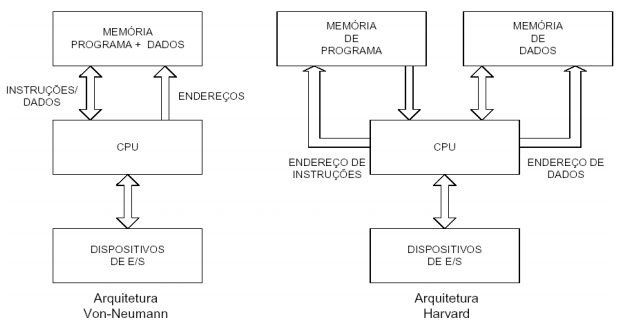
\includegraphics[width=0.8\textwidth]{Arquiteturas.png} \\
  Fonte: \cite{ifsc_figura_arquiteturas}
  \label{fig:arquiteturas}
\end{figure}


\section{Monociclo e caminho de dados}
A organização monociclo é uma das abordagens utilizadas para a implementação de um processador. Nela todas as instruções são lidas, codificadas e executadas durante um único ciclo de clock. Dessa forma, o ciclo de clock precisa durar, no mínimo, o tempo necessário para concluir a instrução mais demorada.

Por um lado, não é muito eficiente, pois há instruções que poderiam ser realizadas de modo mais rápido usando outras abordagens e em razão disso, é um modelo que não é mais implementado em aplicações práticas \cite{cin_monociclo}. Por outro lado, o monociclo possui a vantagem de ser mais simples de compreender e de implementar, o que o torna útil em aplicações didáticas.

Ademais, o caminho de dados compreende o hardware responsável pela execução das instruções. Nele estão presentes registradores, a Unidade Lógica e Aritmética (ULA), barramentos e multiplexadores. Esses componentes trabalham em conjunto para realizar operações como busca da instrução, decodificação, execução e armazenamento de resultados \cite{caminho_dados}. 

A \autoref{fig:cmdados-mips} abaixo apresenta o caminho de dados para um processador MIPS monociclo tradicional.

\begin{figure}[H]
  \centering
  \caption{Caminho de dados MIPS monociclo}
  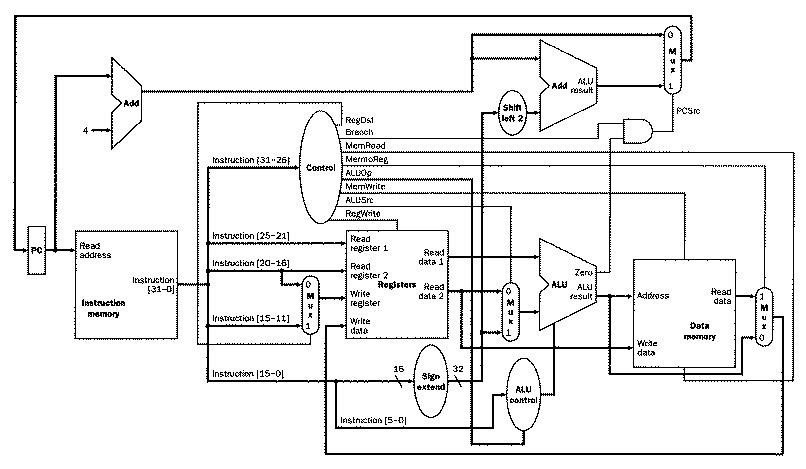
\includegraphics[width=0.8\textwidth]{Imagens/Caminho_dados_mips.jpg} \\
  Fonte: \cite{cda_proc}
  \label{fig:cmdados-mips}
\end{figure}

\section{Modos de endereçamento}
Os modos de endereçamento são responsáveis por especificar como um operando é determinado pelas as instruções. Abaixo, a \autoref{fig:enderecamento} apresenta alguns dos modos de endereçamento. Em seguida são explicados cada um deles de acordo com \cite{stallings2010}.

\begin{figure}[H]
  \centering
  \caption{Tipos de endereçamento}
  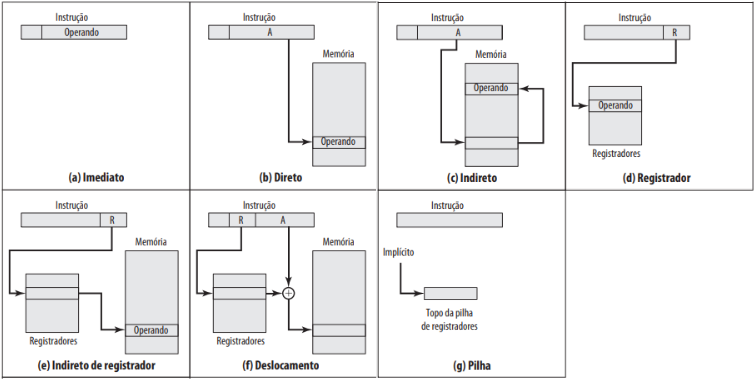
\includegraphics[width=0.8\textwidth]{Imagens/Tipos de endereçamento.png} \\
  Fonte: \cite{stallings2010}
  \label{fig:enderecamento}
\end{figure}

\begin{itemize}
    \item \textbf{Imediato} – O valor do operando é especificado diretamente por meio da instrução.
    \item \textbf{Direto} - A instrução contém o endereço da memória de onde está o operando.
    \item \textbf{Indireto} - Contém um endereço na memória, que por sua vez contém o endereço com o valor operando.
    \item \textbf{Registrador} - A instrução contém o endereço de um registrador com o valor do operando.
    \item \textbf{Indireto de registrador} - É passado o endereço de um registrador, que por sua vez contém um endereço da memória com o valor operando.
    \item \textbf{Deslocamento} - É passado o endereço de um registrador e um imediato. Soma-se o endereço contido no registrador com o valor do imediato para acessar a posição da memória com o operando.
    \item \textbf{Pilha} - O acesso ao operando se dá por meio do acesso à pilha.
\end{itemize}

\section{Formato de instruções}
Para um processador MIPS monociclo, as instruções são compostas por 32 bits. Além disso, contém um Opcode, responsável por identificar qual operação deve ser realizada, além dos operandos. Há uma quantidade variável de operandos de acordo com cada instrução particular. Desse modo, é preciso utilizar mais de um formato de instruções \cite{stallings2010}.

A \autoref{formato_mips} apresenta quais são os formatos de instruções uitlizadas em um modelo MIPS tradicional. Nele, há 3 formatos de instruções: tipo R, tipo I e tipo J. As operações do tipo R envolvem operações de lógica, aritmética e deslocamento, usando três registradores como operandos, sendo dois deles para fornecer os dados e o terceiro para receber.

As instruções do tipo I envolvem operações aritméticas, lógicas, comparação, e acesso à memória. Dois registradores e um imediato são usados como operandos. Por fim, as instruções do tipo J realizam desvios, atualizando o PC para um novo endereço, podendo ser apenas um salto ou um salto com salvamento de retorno.

O campo OP indica Opcode; RS, RT e RD são registradores; shamt é usado para fazer deslocamento de bits e funct é usado para definir a operação a ser realizada pela ULA.

\setlength{\tabcolsep}{15pt} % Define o tamanho das colunas
\begin{table}[H]
\centering
\caption{Formatos de instruções MIPS tradicional}
\label{formato_mips}
\begin{tabular}{|c|c|c|c|c|c|c|}
\hline
Instrução & 6 bits & 5 bits & 5 bits & 5 bits & 5 bits & 6 bits \\
\hline
Tipo R & OP & RS & RT & rd & shamt & funct \\
\hline
Tipo I & OP & RS & RT & \multicolumn{3}{|c|}{Endereço/Imediato} \\
\hline
Tipo J & OP & \multicolumn{5}{|c|}{Endereço de Destino} \\
\hline
\end{tabular}
\vspace{-0.5em}
\begin{center}
Fonte: o Autor.
\end{center}
\end{table}

Note que a quantidade de bits de cada campo é importante para definir certas características do processador. Ao utilizar 6 bits para o Opcode, isso implica que podem haver até \begin{math}2^6 = 64\end{math} operações. Da mesma forma, ao definir 5 bits para os registradores, podem haver até \begin{math}2^5 = 32\end{math} registradores.

\section{FPGA}
Primeiramente, FPGA significa ``Field Programmable Gate Array''. Ele é um circuito integrado, no qual é possível modificar muitas das funcionalidades  por meio de como as portas lógicas e os flip-flop se conectam \cite{intel_fpga}. Ou seja, um componente que, de acordo com os sinais de entrada, permite definir quais devem ser os sinais de saída por meio da programação.

O kit FPGA é, como o nome diz, é um FPGA, porém conectado a uma série de botões, switches, Leds, displays e outros periféricos, que permitem com que os projetos possam ser testados de uma forma simples e prática.

\section{Linguagem Verilog HDL}
A linguagem Verilog foi desenvolvida pela companhia Gateway Design Automation em 1985. Posteriormente, quatro anos depois, essa companhia foi adquirida pela Cadence Design System, que por sua vez, tornou o Verilog domínio público em 1990. Além disso, a linguagem faz parte do padrão IEEE \cite{midorikawa2007}.

O padrão IEEE (Institute of Electrical and Electronic Engineers) é um conjunto de normas técnicas internacionais. Ele proporciona portabilidade, contribuindo para a interconexão de produtos desenvolvidos por empresas distintas \cite{midorikawa2007}.

“O Verilog oferece ao projetista os meios para descrever um sistema digital em vários níveis de abstração, e também suporta ferramentas de projeto para síntese lógica.” \cite{midorikawa2007}. 

Sendo assim, diferente de um circuito esquemático, no qual é desenvolvido usando as portas lógicas e elementos de memória diretamente, o Verilog é responsável por simular o comportamento lógico de uma forma abstrata, sem precisar se importar com as implementações nos mínimos detalhes.


% DESENVOLVIMENTO
\chapter{Desenvolvimento do processador}

\section{Características do projeto}
Para o desenvolvimento do processador foi escolhido como referência o modelo MIPS, pois simplifica a implementação. Porém também foram feitas algumas modificações para atender melhor aos objetivos propostos, como instruções para controlar a pilha; switches; display; esperar; e parar o processamento. Além do mais, seguirá a organização monociclo por ser mais simples de compreender e implementar.

Além disso, o campo de Opcode será composto por 6 bits, de modo que possam haver até 64 instruções. Ademais, serão utilizadas instruções com 32 bits e um total de 64 registradores. Desse modo, serão precisos 6 bits para referenciar um registrador. Do total de registradores, haverão 3 que serão de uso específico e estão apresentados na \autoref{tab:registradores_especificos} abaixo.

\setlength{\tabcolsep}{10pt} % Define o tamanho das colunas
\begin{table}[H]
\centering
\caption{Registradores de uso específico}
\label{tab:registradores_especificos}
\begin{tabular}{|c|l|}
\hline
\textbf{Registrador} & \textbf{Função} \\
\hline
RAL & Armazena o retorno da instrução \textit{jal} \\
\hline
RZ & Armazena o valor zero \\
\hline
RPI & Controla a pilha \\
\hline
\end{tabular}
\vspace{-0.5em}
\begin{center}
Fonte: o Autor.
\end{center}
\end{table}


% Vou deixar de lembrança como foi no início
% RH - Parte alta multiplicação
% HL - Parte baixa multiplicação
% RAL - Registrador que guarda o retorno do jal
% RIN - Recebe o valor dos switches
% ROUT - Envia o valor para a display
% RZ - Zero
% RPI - Controla pilha

Serão utilizados os modos de endereçamento: imediato, para receber valores diretamente; direto, para instruções load e store; registrador, para receber o operando de um registrador; indireto de registrador, para operações load e store; deslocamento, para operações load e store; e por pilha, para controlar a pilha.

\section{Conjunto de instruções}
A \autoref{opcode_lista_bin_zero} abaixo apresenta as instruções escolhidas e o seu respectivo Opcode. Nela, o Opcode recebe um valor em binário, começando do zero.

\setlength{\tabcolsep}{10pt} % Define o tamanho das colunas
\begin{table}[H]
\centering
\caption{Lista numerada das Instruções}
\label{opcode_lista_bin_zero}
\begin{tabular}{|c c|c c|}
\hline
Opcode & Instrução & Opcode & Instrução \\
\hline
\texttt{000000} & halt      & \texttt{010100} & movr     \\
\texttt{000001} & nop       & \texttt{010101} & loaddi   \\
\texttt{000010} & jump      & \texttt{010110} & loadr    \\
\texttt{000011} & jal       & \texttt{010111} & beq      \\
\texttt{000100} & addr      & \texttt{011000} & bne      \\
\texttt{000101} & subr      & \texttt{011001} & blt      \\
\texttt{000110} & mulr      & \texttt{011010} & bgt      \\
\texttt{000111} & divr      & \texttt{011011} & storedi  \\
\texttt{001000} & and       & \texttt{011100} & storer   \\
\texttt{001001} & or        & \texttt{011101} & movi     \\
\texttt{001010} & xnor      & \texttt{011110} & loadi    \\
\texttt{001011} & addi      & \texttt{011111} & in       \\
\texttt{001100} & subi      & \texttt{100000} & pop      \\
\texttt{001101} & muli      & \texttt{100001} & out      \\
\texttt{001110} & divi      & \texttt{100010} & jr       \\
\texttt{001111} & andi      & \texttt{100011} & storei   \\
\texttt{010000} & ori       & \texttt{100100} & push     \\
\texttt{010001} & not       & \texttt{100101} & blet     \\
\texttt{010010} & sl        & \texttt{100110} & lget     \\
\texttt{010011} & sr        &                  &          \\
\hline
\end{tabular}
\vspace{-0.5em}
\begin{center}
Fonte: o Autor.
\end{center}
\end{table}

A partir das instruções, é possível classificá-las de acordo com \autoref{tab:classificacao_instrucoes} abaixo, de modo a atender ao objetivo específico~\ref{objetivo3}.

\setlength{\tabcolsep}{10pt} % Define o tamanho das colunas
\begin{table}[H]
\centering
\caption{Classificação das Instruções}
\label{tab:classificacao_instrucoes}
\begin{tabular}{|c|l|}
\hline
\textbf{Categoria} & \textbf{Instruções} \\
\hline
Operações aritméticas & \textit{addr}, \textit{addi}, \textit{subr}, \textit{subi}, \textit{mulr}, \textit{muli}, \textit{divr}, \textit{divi} \\
\hline
Operações lógicas & \textit{and}, \textit{andi}, \textit{or}, \textit{ori}, \textit{not}, \textit{xnor}, \textit{sl}, \textit{sr} \\
\hline
Desvios condicionais & \textit{beq}, \textit{bne}, \textit{blt}, \textit{bgt}, \textit{blet}, \textit{lget} \\
\hline
Desvios incondicionais & \textit{jump}, \textit{jr}, \textit{jal} \\
\hline
Acesso à memória & \textit{storei}, \textit{storer}, \textit{storedi}, \textit{loadi}, \textit{loadr}, \textit{loaddi} \\
\hline
Movimentação de dados & \textit{movr}, \textit{movi} \\
\hline
Controle da pilha & \textit{push}, \textit{pop} \\
\hline
Acesso aos switches & \textit{in} \\
\hline
Acesso ao display & \textit{out} \\
\hline
Controle de execução & \textit{nop}, \textit{halt} \\
\hline
\end{tabular}
\vspace{-0.5em}
\begin{center}
Fonte: o Autor.
\end{center}
\end{table}


A \autoref{opcode1} e a \autoref{opcode2} contêm a operação a ser realizada por cada uma das instruções apresentadas acima, além de separar as instruções em nove formatos. Nela, ``<='' indica uma atribuição; RD, RS e RT são registradores; IM indica imediato; END representa o endereço; MEM indica acesso à memória; PILHA indica acesso à pilha. 

Ainda sobre a \autoref{opcode1} e a \autoref{opcode2}, o símbolo ``\textasciitilde'' indica uma inversão bit a bit. O número, quando ele aparece, indica o número de bits. A expressão ``+RPI'' indica que primeiro incrementa RPI e depois usa o valor, enquanto ``RPI-'' indica que primeiro usa o valor e depois decrementa.

\setlength{\tabcolsep}{10pt}
\begin{table}[H]
\centering
\caption{Instruções utilizadas e operações realizadas separadas por formato (Parte 1)}
\label{opcode1}
\begin{tabular}{|c|>{\raggedright\arraybackslash}p{7cm}|}
\hline
Instrução & Operação\\
\hline
\multicolumn{2}{|c|}{Formato 1} \\
\hline
addr & RD <= RS + RT \\
subr & RD <= RS - RT \\
mulr & RD <= RS * RT \\
divr & RD <= RS / RT \\
and & RD <= RS and RT \\
or & RD <= RS or RT \\
xnor & RD <= RS xnor RT \\
\hline
\multicolumn{2}{|c|}{Formato 2} \\
\hline
addi & RD <= RS + IM14 \\
subi & RD <= RS - IM14 \\
muli & RD <= RS * IM14 \\
divi & RD <= RS / IM14 \\
andi & RD <= RS and IM14 \\
ori & RD <= RS or IM14 \\
not & RD <= \textasciitilde RS \\
sl & RD <= RS deslocado IM14 esq \\
sr & RD <= RS deslocado IM14 dir \\
movr & RD <= RS \\
loaddi & RD <= MEM(RS + END14) \\
loadr & RD <= MEM(RS) \\
\hline
\multicolumn{2}{|c|}{Formato 3} \\
\hline
beq & if(RS == RT) PC <= PC+1+END14 \\
bne & if(RS != RT) PC <= PC+1+END14 \\
blt & if(RS < RT) PC <= PC+1+END14 \\
bgt & if(RS > RT) PC <= PC+1+END14 \\
blet & if(RS <= RT) PC <= PC+1+END14 \\
lget & if(RS >= RT) PC <= PC+1+END14 \\
storedi & MEM(RS + END14) <= RT \\
storer & MEM(RS) <= RT \\
\hline
\multicolumn{2}{|c|}{Formato 4} \\
\hline
movi & RD <= IM20 \\
loadi & RD <= MEM(END20) \\
in & RD <= SWITCHES \\
pop & RD <= PILHA(RPI-) \\
\hline
\multicolumn{2}{|c|}{Formato 5} \\
\hline
out & DISPLAY <= RS \\
jr & PC <= RS \\
\hline
\end{tabular}
\vspace{-0.5em}
\begin{center}
\textit{Fonte: o Autor.}
\end{center}
\end{table}


\setlength{\tabcolsep}{10pt}
\begin{table}[H]
\centering
\caption{Instruções utilizadas e operações realizadas separadas por formato (Parte 2)}
\label{opcode2}
\begin{tabular}{|c|>{\raggedright\arraybackslash}p{7cm}|}
\hline
Instrução & Operação\\
\hline
\multicolumn{2}{|c|}{Formato 6} \\
\hline
storei & MEM(END20) <= RT \\
push & PILHA(+RPI) <= RT \\
\hline
\multicolumn{2}{|c|}{Formato 7} \\
\hline
halt & Para o processador \\
nop & Aguarda um ciclo de clock \\
jump & PC <= END26 \\
jal & RAL <= PC; PC <= END26 \\
\hline
\end{tabular}
\vspace{-0.5em}
\begin{center}
\textit{Fonte: o Autor.}
\end{center}
\end{table}

Observe que há três instruções distintas para load e para store e elas mudam a forma como o endereço da memória é obtido: loadi e storei usam um imediato; loadr e storer usam o endereço contido em um registrador; loadd e strored usam o endereço contido em um registrador somado com um imediato. 

Seguindo uma lógica parecida, há as funções de salto incondicional: jmp, realiza um salto para o endereço de um imediato; jr, para um endereço guardado em um registrador; e jal, funciona como um jmp, porém também armazena o valor do retorno em RAL.

Além do mais, repare que há muitas instruções que possuem duas versões: uma usando somente registradores e outra, na qual o nome da instrução termina com a letra ``i'', utilizando registradores e imediato. 

Além disso, há instruções especiais como: in e out, que recebem a entrada dos switches e enviam o display, respectivamente;
nop e hlt, responsáveis, respectivamente, por aguardar um ciclo de clock e parar o processador.

Ademais, nota-se que dentro de cada um dos formatos são sempre utilizados os mesmos registradores de uso geral (RD, RS e RT) e imediatos do mesmo tipo e tamanho. Na próxima seção é apresentado detalhadamente cada um dos formatos e como serão organizadas as suas instruções.

\section{Formato de instruções}

Como dito anteriormente, foram feitas algumas adaptações no modelo MIPS, de modo que para o projeto são usados nove formatos de instrução ao invés de apenas três. Além do mais, como os formatos definidos dependem dos registradores e dos imediatos/endereços usados, eles são distintos dos apresentados na \autoref{tab:classificacao_instrucoes}.

Desse modo, a \autoref{formato12} apresenta como serão preenchidos os bits para as instruções de cada um dos formatos. Os campos com o símbolo ``-'' indicam que ele não é usado. 

\setlength{\tabcolsep}{15pt} % Define o tamanho das colunas
\begin{table}[H]
\centering
\caption{Todos os formatos de instruções}
\label{formato12}
\begin{tabular}{|c|c|c|c|c|c|}
\hline
Bits & 31 - 26 & 25 - 20 & 19 - 14 & 13 - 8 & 7 - 0 \\
\hline
Formato 1 & OP & RD & RS & RT & - \\
\hline
Formato 2 & OP & RD & RS & \multicolumn{2}{|c|}{IM14/END14/-} \\
\hline
Formato 3 & OP & RS & RT & \multicolumn{2}{|c|}{END14/-} \\
\hline
Formato 4 & OP & RD & \multicolumn{3}{|c|}{IM20/END20/-} \\
\hline
Formato 5 & OP & RS & \multicolumn{3}{|c|}{-} \\
\hline
Formato 6 & OP & RT & \multicolumn{3}{|c|}{END20/-} \\
\hline
Formato 7 & OP & \multicolumn{4}{|c|}{END26/-} \\
\hline
\end{tabular}
\vspace{-0.5em}
\begin{center}
Fonte: o Autor.
\end{center}
\end{table}

Conforme a \autoref{opcode1} e a \autoref{opcode2}, as instruções que pertencem a cada um dos formatos estão apresentadas na \autoref{tab:formatos_instrucoes} abaixo:

\setlength{\tabcolsep}{10pt} % Define o tamanho das colunas
\begin{table}[H]
\centering
\caption{Classificação das Instruções por Formato}
\label{tab:formatos_instrucoes}
\begin{tabular}{|c|l|}
\hline
\textbf{Formato} & \textbf{Instruções} \\
\hline
Formato 1 & \textit{add}, \textit{sub}, \textit{mul}, \textit{div}, \textit{and}, \textit{or}, \textit{xnor} \\
\hline
Formato 2 & \textit{addi}, \textit{subi}, \textit{muli}, \textit{divi}, \textit{andi}, \textit{ori}, \textit{not}, \textit{sl}, \textit{sr}, \textit{mov}, \textit{loadd}, \textit{loadr} \\
\hline
Formato 3 & \textit{beq}, \textit{bne}, \textit{blt}, \textit{bgt}, \textit{blet}, \textit{lget}, \textit{storedi}, \textit{storer} \\
\hline
Formato 4 & \textit{movi}, \textit{loadi}, \textit{in}, \textit{pop} \\
\hline
Formato 5 &  \textit{out}, \textit{jr} \\
\hline
Formato 6 & \textit{storei}, \textit{push}  \\
\hline
Formato 7 & \textit{hlt}, \textit{nop}, \textit{jmp}, \textit{jal} \\
\hline
\end{tabular}
\vspace{-0.5em}
\begin{center}
Fonte: o Autor.
\end{center}
\end{table}

\section{Caminho de dados}
A partir de tudo o que foi definido nas seções anteriores, é possível desenvolver o circuito do processador. A função dele é apresentar qual deverá ser o caminho que os dados devem passar para realizar a operação de cada uma das instruções.

Como o processador desenvolvido foi baseado no MIPS, há muita similaridade no caminho de dados, porém foi preciso adicionar novos elementos para comportar todas as instruções e os dispositivos de entrada e saída. A \autoref{fig:cmdados} apresenta o caminho de dados para o processador que será desenvolvido.

\begin{figure}[H]
  \centering
  \caption{Caminho de dados}
  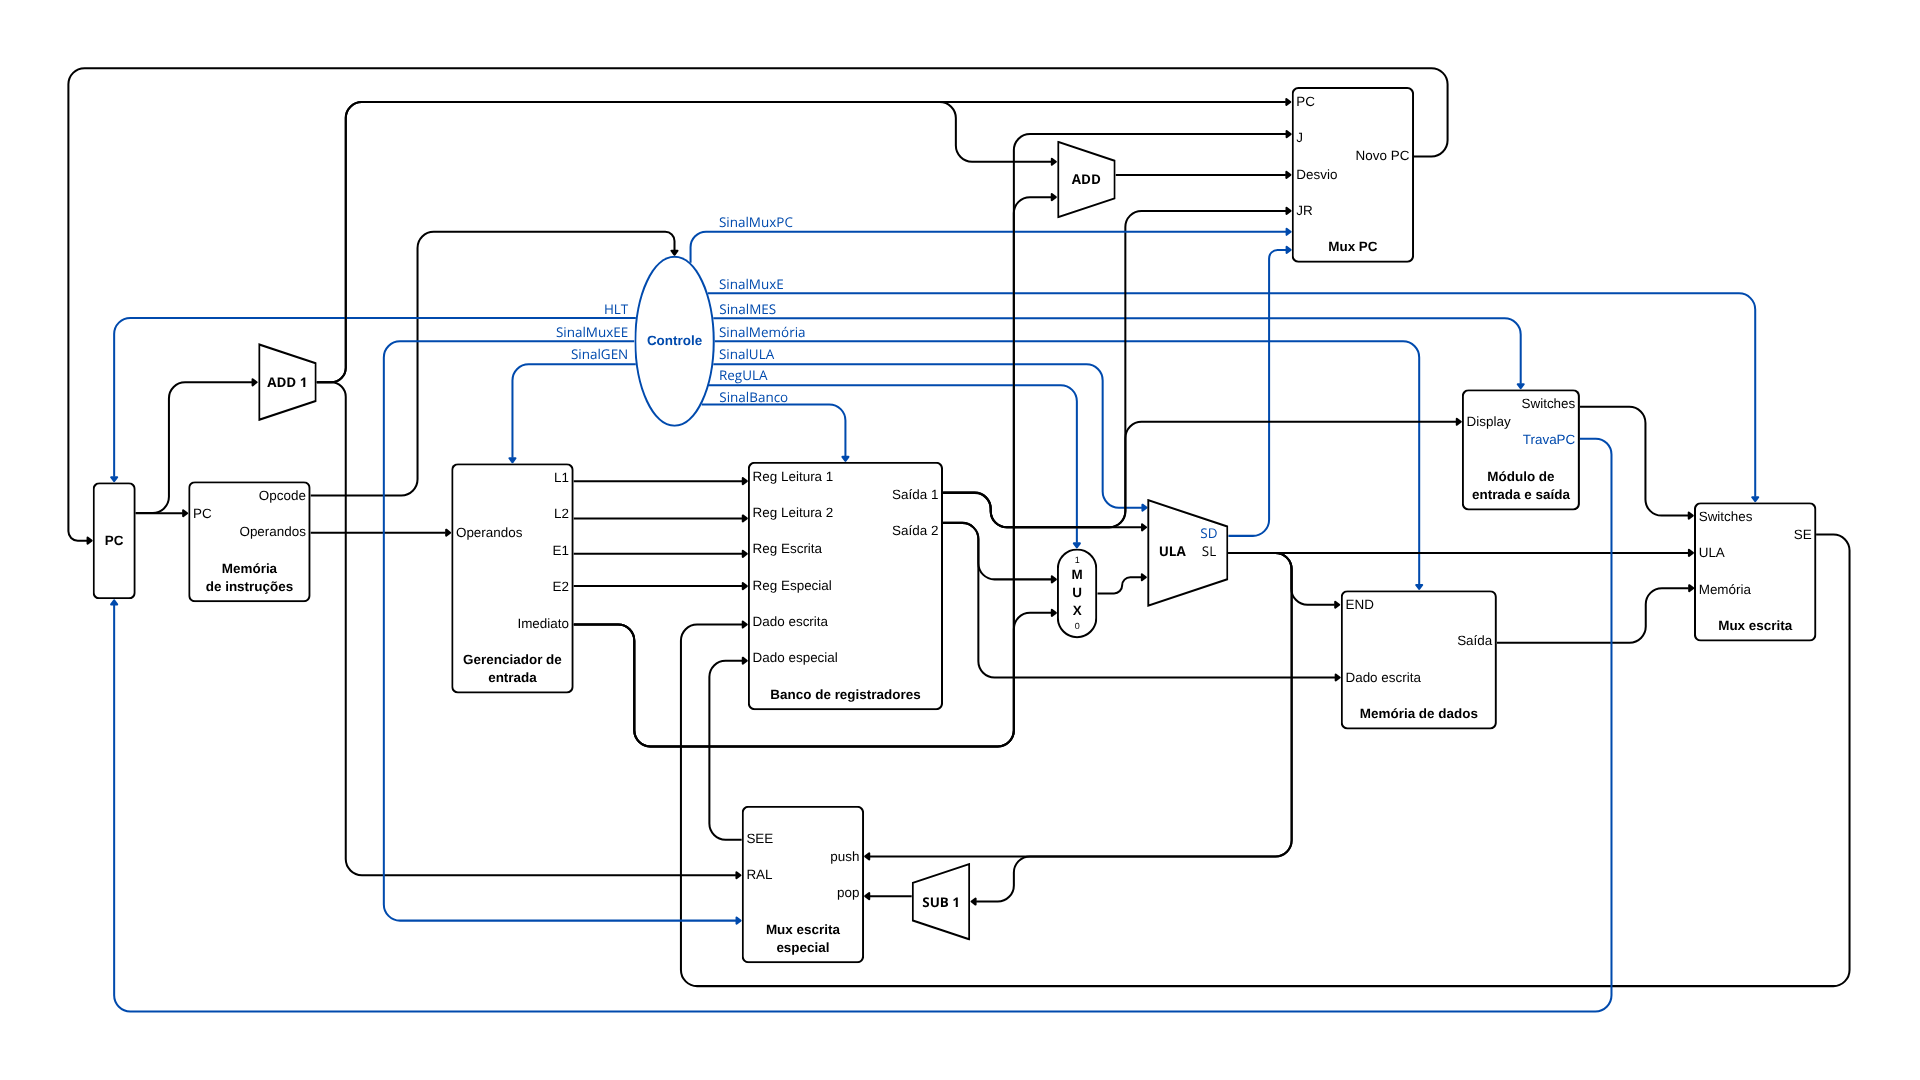
\includegraphics[width=0.8\textwidth]{Imagens/CmDados_Novo.png} \\
  Fonte: o Autor.
  \label{fig:cmdados}
\end{figure}

Note que foi adicionado um módulo chamado ``Gerenciador de entrada''. Ele é responsável por definir quais serão os registradores que serão utilizados para leitura (L1 e L2) e para a escrita (E1 e E2) no banco de registradores. Ademais, ele identifica qual será o imediato que será utilizado e estende-o para 32 bits.

Além do mais, há dois campos para escrita no banco de registradores: ``Reg escrita'' e ``Reg especial'', que recebem os dados, respectivamente, de ``Dado escrita'' e ``Dado especial''. O primeiro deles é utilizado para escrever nos registradores especificados nas instruções, enquanto o segundo, o ``especial'', escreve em registradores específicos: RPI (push/pop) ou RAL. Isso é necessário pois as  instruções push, pop e jal utilizam registradores específicos para funcionarem e no caso de pop, é preciso escrever em dois registradores ao mesmo tempo.

Além disso, foram adicionados três multiplexadores (MUX): um para gerenciar o próximo valor do PC, um segundo para definir qual dado será enviado para a escrita no banco de registradores e um terceiro utilizado para definir o dado da escrita especial. A função deles é selecionar apenas um dos sinais de entrada e torná-lo o sinal de saída do módulo.

Ademais, foi inserido o ``Módulo de entrada e saída'', usado para enviar os dados para o display e para receber os dados dos switches.

A \autoref{tab:sinais_de_controle} abaixo apresenta quais são todos os sinais de controle utilizados e qual é o papel de cada um no circuito. Para a implementação, somente os sinais HLT, SinalMemória, RegULA, SD e TravaPC são binários, os demais são compostos por mais de um bit.

\setlength{\tabcolsep}{10pt} % Define o tamanho das colunas
\begin{table}[H]
\centering
\caption{Sinais de controle e suas funções}
\label{tab:sinais_de_controle}
\begin{tabular}{|c|l|}
\hline
\textbf{Nome} & \textbf{Função} \\
\hline
HLT & Quando ativo, impede o PC de ser incrementado \\
\hline
SinalMuxEE & Determina o dado para escrita especial \\
\hline
SinalGEN & Estabelece os registradores e o imediato que serão usados \\
\hline
SinalMuxPC & Define qual será o próximo valor do PC \\
\hline
SinalMuxE & Determina o dado para escrita \\
\hline
SinalMES & \makecell[l]{Indica se serão enviados dados para o display ou lido dados dos \\ switches} \\
\hline
SinalMemória & Define quando será feita a escrita de dados na memória \\
\hline
SinalULA & Aponta a operação a ser feita pela ULA \\
\hline
RegULA &  \makecell[l]{Indica se o dado da segunda entrada da ULA virá de um registrador \\ ou imediato} \\
\hline
SinalBanco & Estabelece se será feita uma escrita e/ou escrita especial \\
\hline
SD & Sinal de saída da ULA que indica se haverá desvio ou não \\
\hline
TravaPC & \makecell[l]{Sinal de saída do módulo de entrada e saída que impede o PC \\ de incrementar até um botão do FPGA ser apertado} \\
\hline
\end{tabular}
\vspace{-0.5em}
\begin{center}
Fonte: o Autor.
\end{center}
\end{table}

Em sequência, as figuras: \autoref{fig:cmdados-f1}, \autoref{fig:cmdados-f3-desvios} e \autoref{fig:cmdados-f7-pop} apresentam o caminho de dados executados por algumas instruções. Neles, estão em vermelho os caminhos de dados que são usados e em verde os sinais de controle utilizados.

Observe que dentro de um mesmo formato é possível que haja um ou mais caminhos distintos para as instruções. Além disso, os demais caminhos podem ser obtidos tomando como referência os já apresentados, os sinais de controle e considerando a \autoref{opcode1} e \autoref{opcode2}.

O primeiro caminho de dados, apresentado pela \autoref{fig:cmdados-f1}, mostra o caminho de dados das instruções do formato 1. Nele, assim como em todas as instruções, é lido o valor da memória de instruções apontada pelo PC e, em seguida, são determinados os registradores a serem usados.

Nesse caso, serão lidos os valores de dois registradores, RS e RT, e serão escritos dados no registrador RD. Os dados lidos são enviados para a ULA, que realiza a operação de acordo com o Opcode da instrução. Em sequência, o valor de saída da ULA é selecionado para ser usado para escrita.

Enquanto isso ocorre, o valor do PC é incrementado em 1 para acessar a próxima instrução, passa pelo Mux PC e é enviado para atualizar o valor do PC.

\begin{figure}[H]
  \centering
  \caption{Caminho de dados - Formato 1 (add, sub, mul, div, and, or, xnor)}
  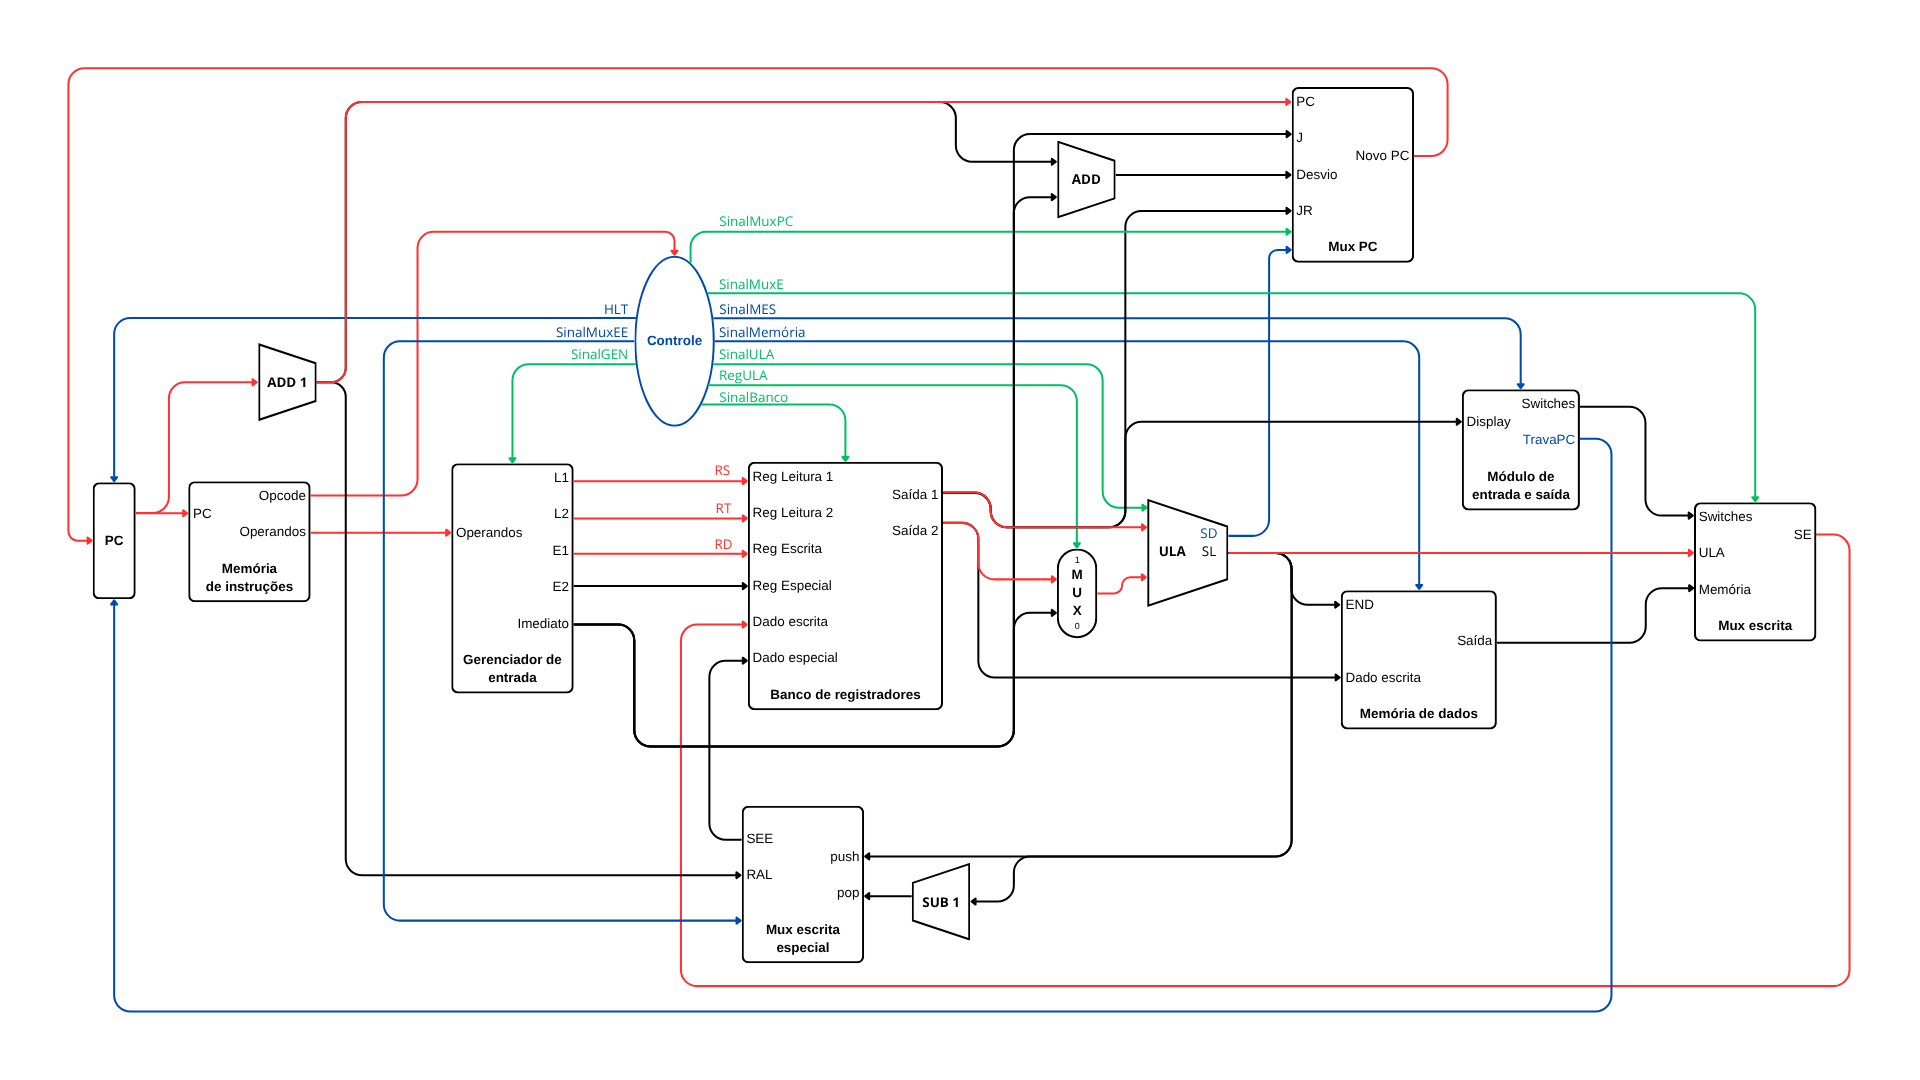
\includegraphics[width=0.7\textwidth]{Imagens/CmDados_Novo-f1.png} \\
  Fonte: o Autor.
  \label{fig:cmdados-f1}
\end{figure}

A \autoref{fig:cmdados-f3-desvios} apresenta o caminho de dados para desvios condicionais tomados. Nela, é possível observar o caminho de dados para as instruções beq, bne, blt, bgt, blet e lget.

Nela é lida a instrução com base no endereço do PC e definidos dois registradores, RD e RS, para leitura e um imediato usado para o desvio. 

Nesse caso, o SinalBanco é usado para indicar que não haverá escrita. Sendo assim, são apenas lidos dois registradores do banco de registradores e enviados à ULA para serem comparados. 

Em sequência, a ULA envia o sinal de controle SD para indicar que o desvio será tomado e, após isso, o valor do PC é atualizado de acordo com o valor do PC atual somado com o valor do imediato passado.

\begin{figure}[H]
  \centering
  \caption{Caminho de dados - Formato 3 desvio tomado (beq, bne, blt, bgt)}
  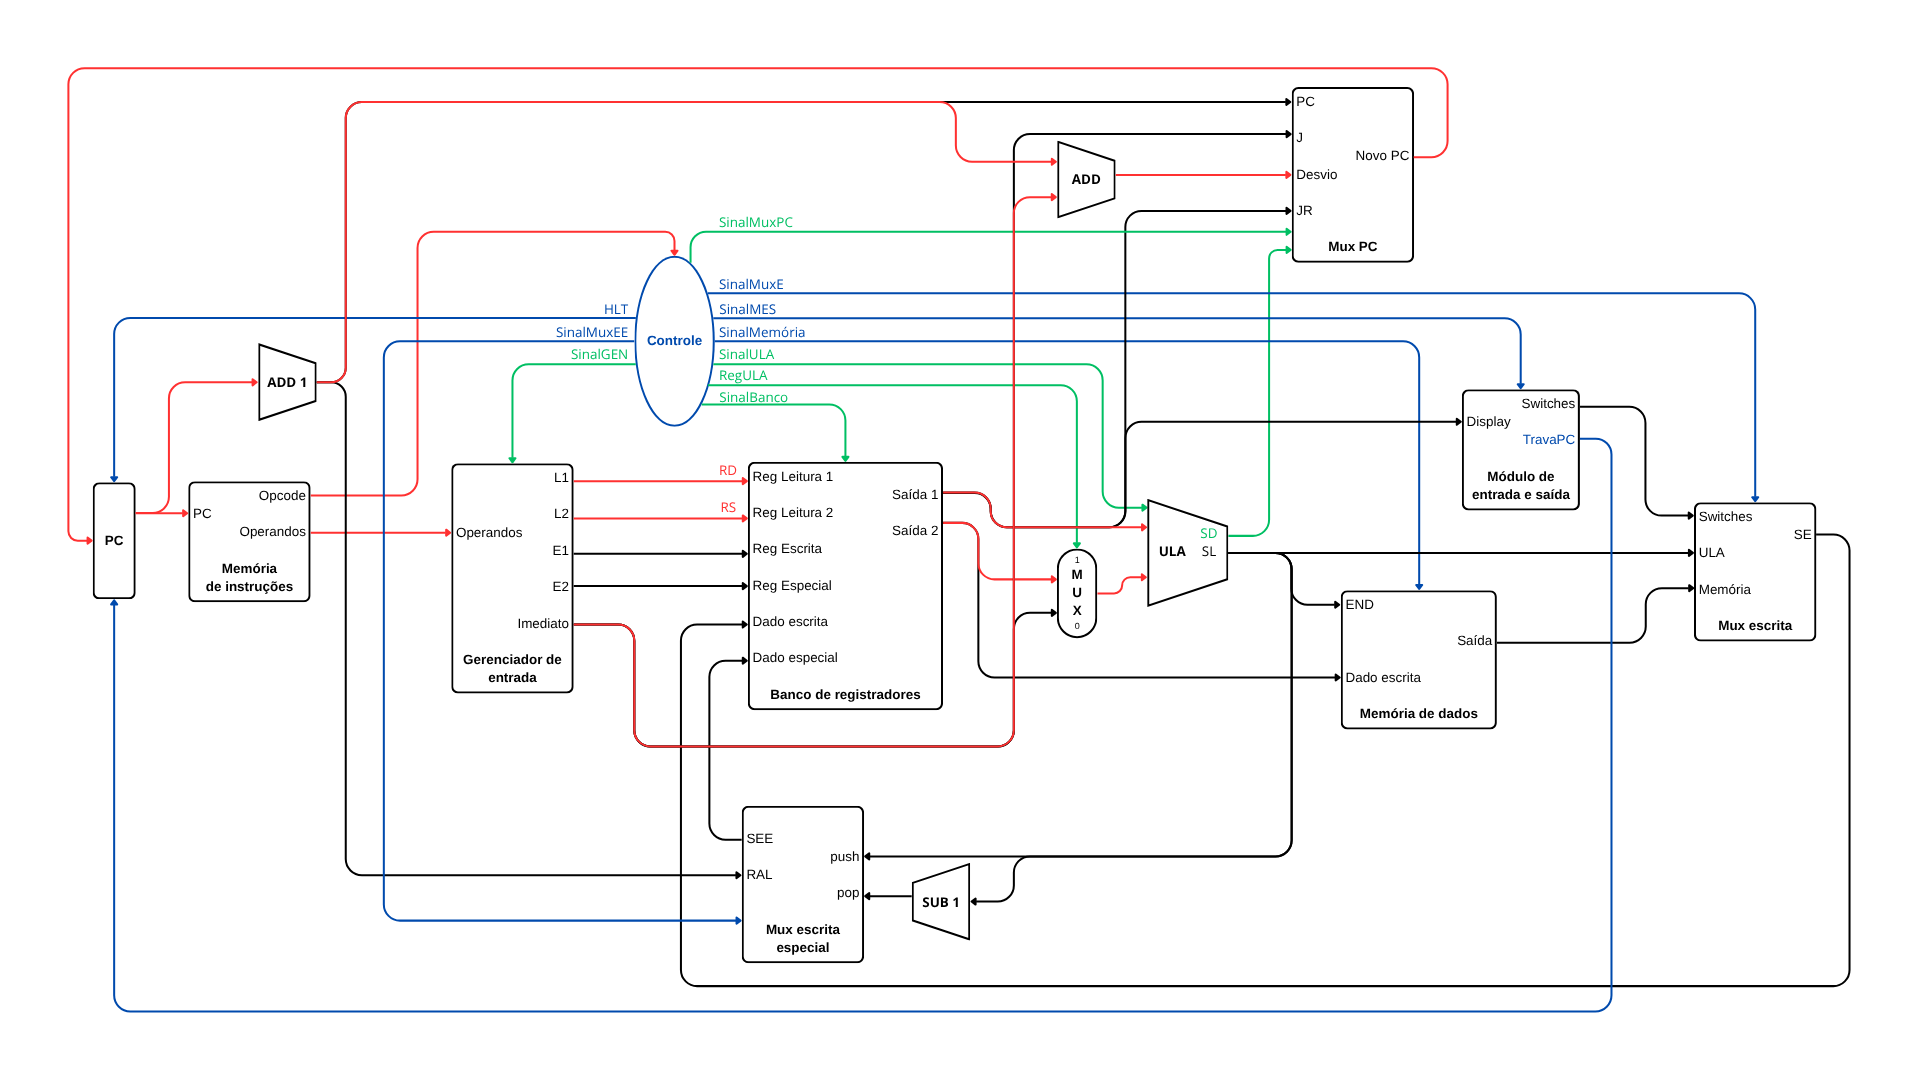
\includegraphics[width=0.7\textwidth]{Imagens/CmDados_Novo-f3-Desvios.png} \\
  Fonte: o Autor.
  \label{fig:cmdados-f3-desvios}
\end{figure}

Por fim, a \autoref{fig:cmdados-f7-pop} apresenta o caminho de dados para a instrução pop. Nele, é lida a instrução na memória de instruções, em seguida, o gerenciador de entrada determina o registrador especial RPI tanto para a leitura, para ele fornecer o endereço da pilha, quanto para a escrita, para atualizar o valor dele. Além do registrador RD usado para receber o dado do pop.

O registrador lido é enviado para ULA, onde ele é enviado diretamente para a saída usando  o código 01110 presente na \autoref{tab:op_ula}. O endereço é enviado para a entrada da memória de dados, onde o SinalMemória determina que será feita uma leitura no endereço. O dado lido passa pelo mux de escrita e é levado para ser armazenado em RD. 

Enquanto isso, da saída da ULA o endereço é decrementado em 1, para apontar para a última posição de memória ocupada, passa pelo mux de escrita especial e é usado para atualizar o endereço contido em RPI. Simultaneamente, o PC é incrementado em 1 e atualizado.

\begin{figure}[H]
  \centering
  \caption{Caminho de dados - Formato 7 (pop)}
  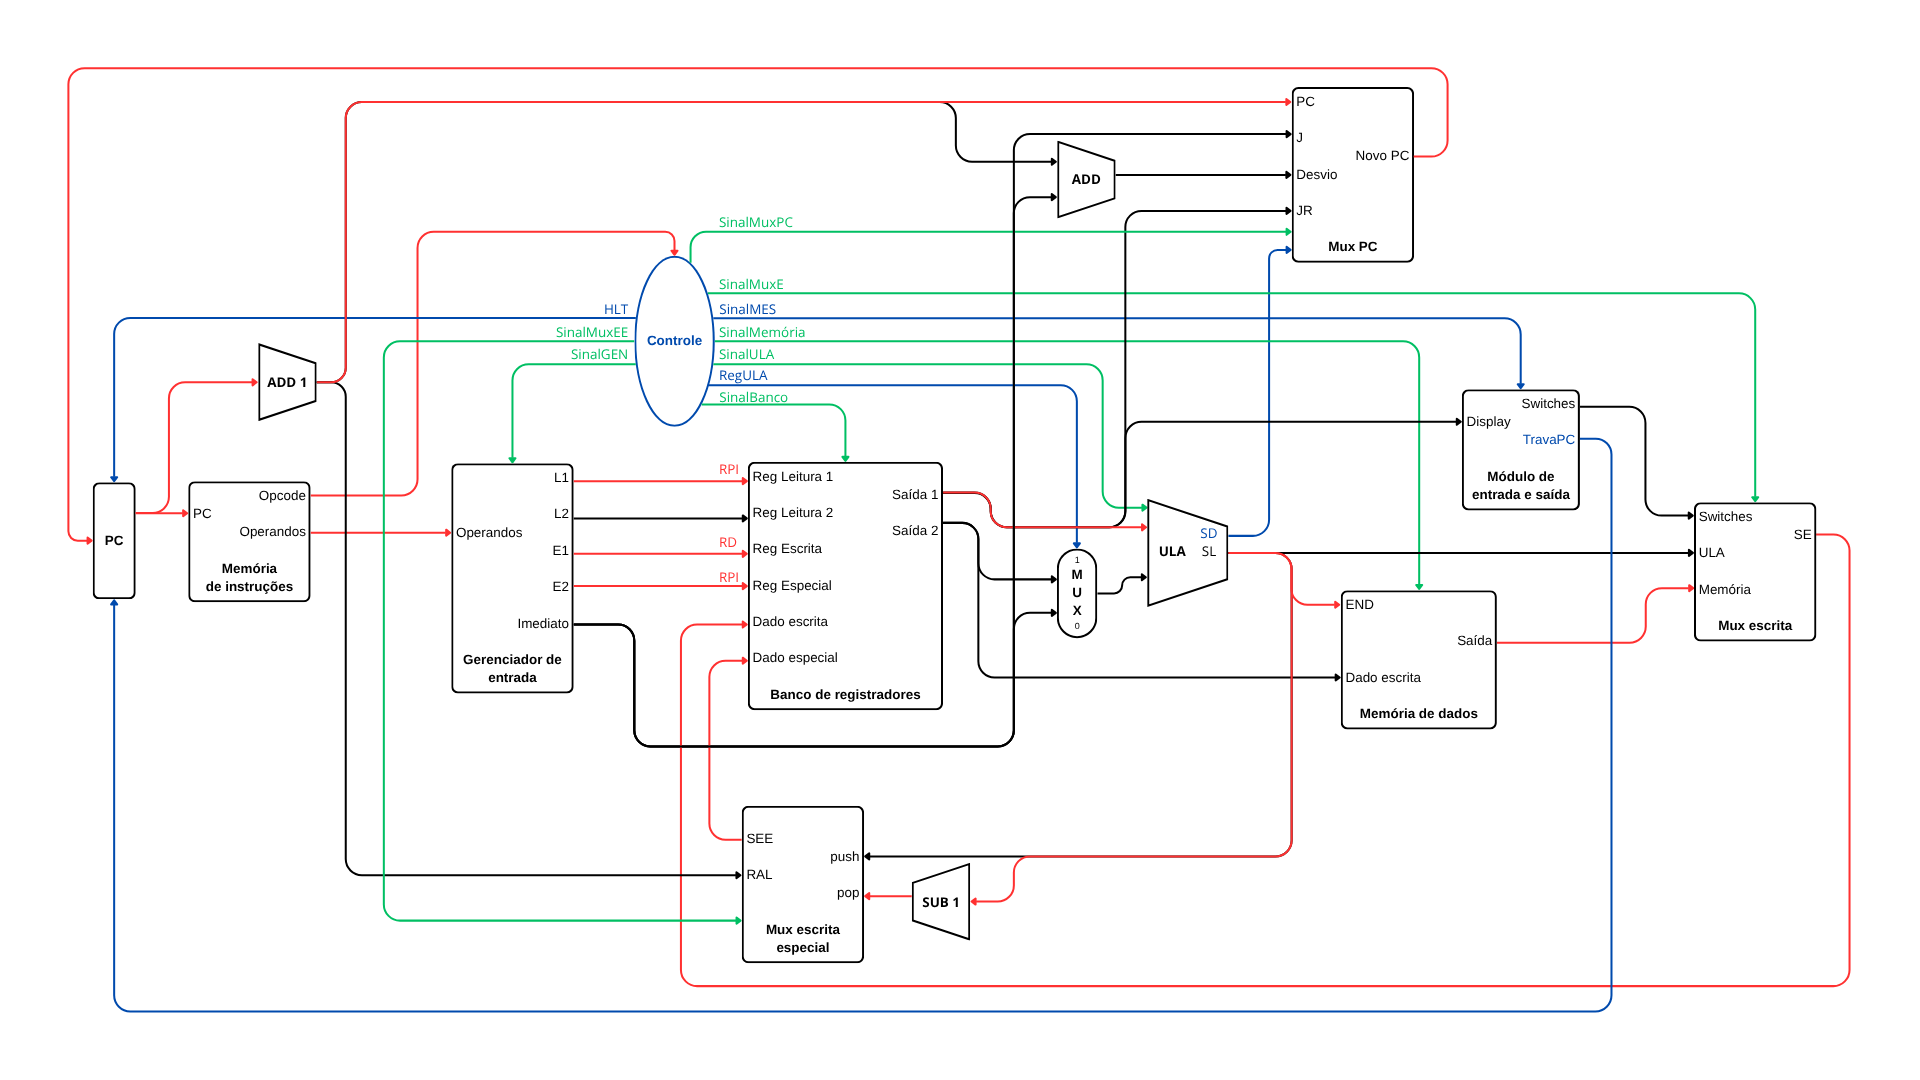
\includegraphics[width=0.7\textwidth]{Imagens/CmDados_Novo-f7-pop.png} \\
  Fonte: o Autor.
  \label{fig:cmdados-f7-pop}
\end{figure}


% -----------------------------------------------------------------
% -------------------------- DESENVOLVIMENTO ----------------------
% -----------------------------------------------------------------
\section{Descrição dos módulos}
\subsection{ULA}
No início da implementação do projeto, foi desenvolvida a unidade de lógica e aritmética (ULA), responsável por fazer as operações de lógica, aritmética e determinar se os desvios vão ou não ocorrer. Todas as entradas e saídas utilizadas, bem como o seu papel, estão presentes na \autoref{tab:IO-ULA} abaixo.

\setlength{\tabcolsep}{10pt}
\begin{table}[H]
\centering
\caption{Entradas e saídas do módulo da ULA}
\label{tab:IO-ULA}
\begin{tabular}{|c|c|l|}
\hline
\multicolumn{3}{|c|}{\textbf{ENTRADAS}} \\
\hline
\textbf{Sinal} & \textbf{Nº bits} & \textbf{Descrição} \\
\hline
EA & 32 & Primeiro operando \\
\hline
EB & 32 & Segundo operando \\
\hline
SinalULA & 5 & Sinal de controle que define a operação da ULA \\
\hline
\multicolumn{3}{|c|}{\textbf{SAÍDAS}} \\
\hline
\textbf{Sinal} & \textbf{Nº bits} & \textbf{Descrição} \\
\hline
SL & 32 & Saída padrão com o resultado da operação \\
\hline
SD & 1 & Indica desvio condicional (1=sim, 0=não) \\
\hline
\end{tabular}
\vspace{-0.5em}
\begin{center}
Fonte: o Autor.
\end{center}
\end{table}

A \autoref{tab:op_ula}, abaixo, segue a nomenclatura apresentada na \autoref{tab:IO-ULA} e apresenta detalhadamente quais são as instruções que utilizam cada um dos valores de SinalULA, bem como qual é a operação realizada em cada um dos casos.

\begin{table}[H]
\centering
\caption{Operações realizadas pela ULA conforme o SinalULA}
\label{tab:op_ula}
\begin{tabular}{|c|l|l|}
\hline
\textbf{SinalULA} & \textbf{Instrução} & \textbf{Operação} \\
\hline
00000 & add  & SL = EA + EB \\
00001 & sub  & SL = EA - EB \\
00010 & and  & SL = EA \& EB \\
00011 & or   & SL = EA | EB \\
00100 & not  & SL = \textasciitilde EA \\
00101 & xnor & SL = EA \textasciitilde{}\^{} EB \\
00110 & sl   & SL = EA \textless\textless{} EB[4:0] \\
00111 & sr   & SL = EA \textgreater\textgreater{} EB[4:0] \\
01000 & beq  & SD = (EA == EB) \\
01001 & bne  & SD = (EA != EB) \\
01010 & blt  & SD = (EA < EB) \\
01011 & bgt  & SD = (EA > EB) \\
01100 & mul  & SL = EA * EB \\
01101 & div  & SL = EA / EB \\
01110 & pop/mov EA & SL = EA \\
01111 & movi & SL = EB \\
10000 & push & SL = EA + 1 \\
\hline
\end{tabular}
\vspace{-0.5em}
\begin{center}
Fonte: o Autor.
\end{center}
\end{table}

Note que existem instruções especiais nas três últimas linhas da \autoref{tab:op_ula}, nas quais a operação realizada é consideravelmente diferente do nome das instruções. Isso ocorre pois para simplificar o processo de implementação dessas instruções foi criada uma operação especial para a ULA.

Para a instrução pop, a entrada EA vai receber como entrada o valor do registrador RPI e deve enviar como saída o próprio valor de RPI inalterado para acessar a pilha. No caso do mov, a entrada EA vai receber o valor de um registrador e a saída deve ser o mesmo valor da entrada para ser salvo em outro registrador.

No caso do movi, a entrada EB vai receber um imediato e esse imediato deverá ser salvo em um registrador, logo a saída da ULA deve ser o próprio EB. Para o push, de modo similar ao pop, a entrada EA recebe o valor de RPI, porém é preciso incrementar em 1 esse valor para acessar corretamente os endereços da pilha, portanto, nesse caso a saída é EA somado com 1.

Além do mais, SD só é utilizado em operações de desvio condicional. Em operações que não são de desvio condicional, a saída SD permanece com o sinal zero. Do mesmo modo, em operações de desvio condicional, o valor da saída SL permanece como zero.

\subsection{Banco de registradores}

O banco de registradores tem o papel de definir quais serão os registradores lidos e/ou escritos. Todas as entradas e saídas utilizadas estão presentes na \autoref{tab:IO-banco_registradores}.

\setlength{\tabcolsep}{10pt} % Define o tamanho das colunas
\begin{table}[H]
\centering
\caption{Entradas e saídas do módulo do banco de registradores}
\label{tab:IO-banco_registradores}
\begin{tabular}{|c|c|l|}
\hline
\multicolumn{3}{|c|}{\textbf{ENTRADAS}} \\
\hline
\textbf{Sinal} & \textbf{Nº bits} & \textbf{Descrição} \\
\hline
clock & 1 & Controla a escrita, feita somente na borda de subida \\
\hline
reg\_leitura1 & 6 & Endereço do primeiro registrador a ser lido \\
\hline
reg\_leitura2 & 6 & Endereço do segundo registrador a ser lido \\
\hline
reg\_escrita & 6 & Endereço do registrador de escrita \\
\hline
reg\_especial & 6 & Endereço do registrador especial \\
\hline
dado\_escrita & 32 & Valor a ser escrito no registrador de escrita \\
\hline
dado\_especial & 32 & Valor a ser escrito no registrador especial \\
\hline
SinalBanco[0] & 1 & Habilita escrita no registrador de escrita (1=sim, 0=não) \\
\hline
SinalBanco[1] & 1 & Habilita escrita no registrador especial (1=sim, 0=não) \\
\hline
\multicolumn{3}{|c|}{\textbf{SAÍDAS}} \\
\hline
\textbf{Sinal} & \textbf{Nº bits} & \textbf{Descrição} \\
\hline
saida1 & 32 & Valor lido no primeiro registrador \\
\hline
saida2 & 32 & Valor lido no segundo registrador \\
\hline
\end{tabular}
\vspace{-0.5em}
\begin{center}
Fonte: o Autor.
\end{center}
\end{table}

Note que na implementação há um único ``SinalBanco'' de 2 bits, porém na tabela seus bits foram apresentados separadamente. Isso foi feito para evidenciar que o valor dos bits são independentes entre si, com o bit menos significativo, [0], sendo responsável pela escrita e o mais significativo, [1], responsável pela escrita especial.

Além disso, observe que o registrador de escrita recebe exclusivamente o valor de dado\_escrita e o registrador especial recebe exclusivamente o valor de dado\_especial. Ademais, ambas as escritas ocorrem somente na borda de subida do clock.

Sobre as saídas, ambas as saídas são feitas de modo assíncrono, ou seja, não dependem do sinal do clock. A saida1 sempre envia o valor do primeiro registrador lido e a saida2 o valor do segundo registrador lido.

O banco foi desenvolvido como uma matriz de 32 posições, correspondentes aos 32 bits de cada registrador, por 64, correspondentes ao número de registradores.

\subsection{Integração do banco de registrador e  ULA}
\label{secao_integracao_ULA_banco}
Para essa etapa foi feito um recorte de três módulos do caminho de dados: o banco de registradores, a ULA e o multiplexador. Desse modo, foi preciso usar os dois módulos desenvolvidos anteriormente e criar um novo para o multiplexador. 

Primeiramente, sobre o multiplexador, ele é um módulo que recebe dois valores de 32 bits e um bit de controle, que define se a saída, também de 32 bits, será o primeiro valor recebido (1) ou o segundo (0).

A \autoref{fig:cmdados_unidade_processamento} abaixo apresenta o caminho de dados utilizado para a implementação desse módulo. Note que ele é similar ao caminho de dados do processador, presente na \autoref{fig:cmdados}, porém foram removidos alguns módulos e colocadas algumas saídas a mais para acompanhar o valor lido pelo banco.

\begin{figure}[H]
  \centering
  \caption{Caminho de dados - Formato 7 (pop)}
  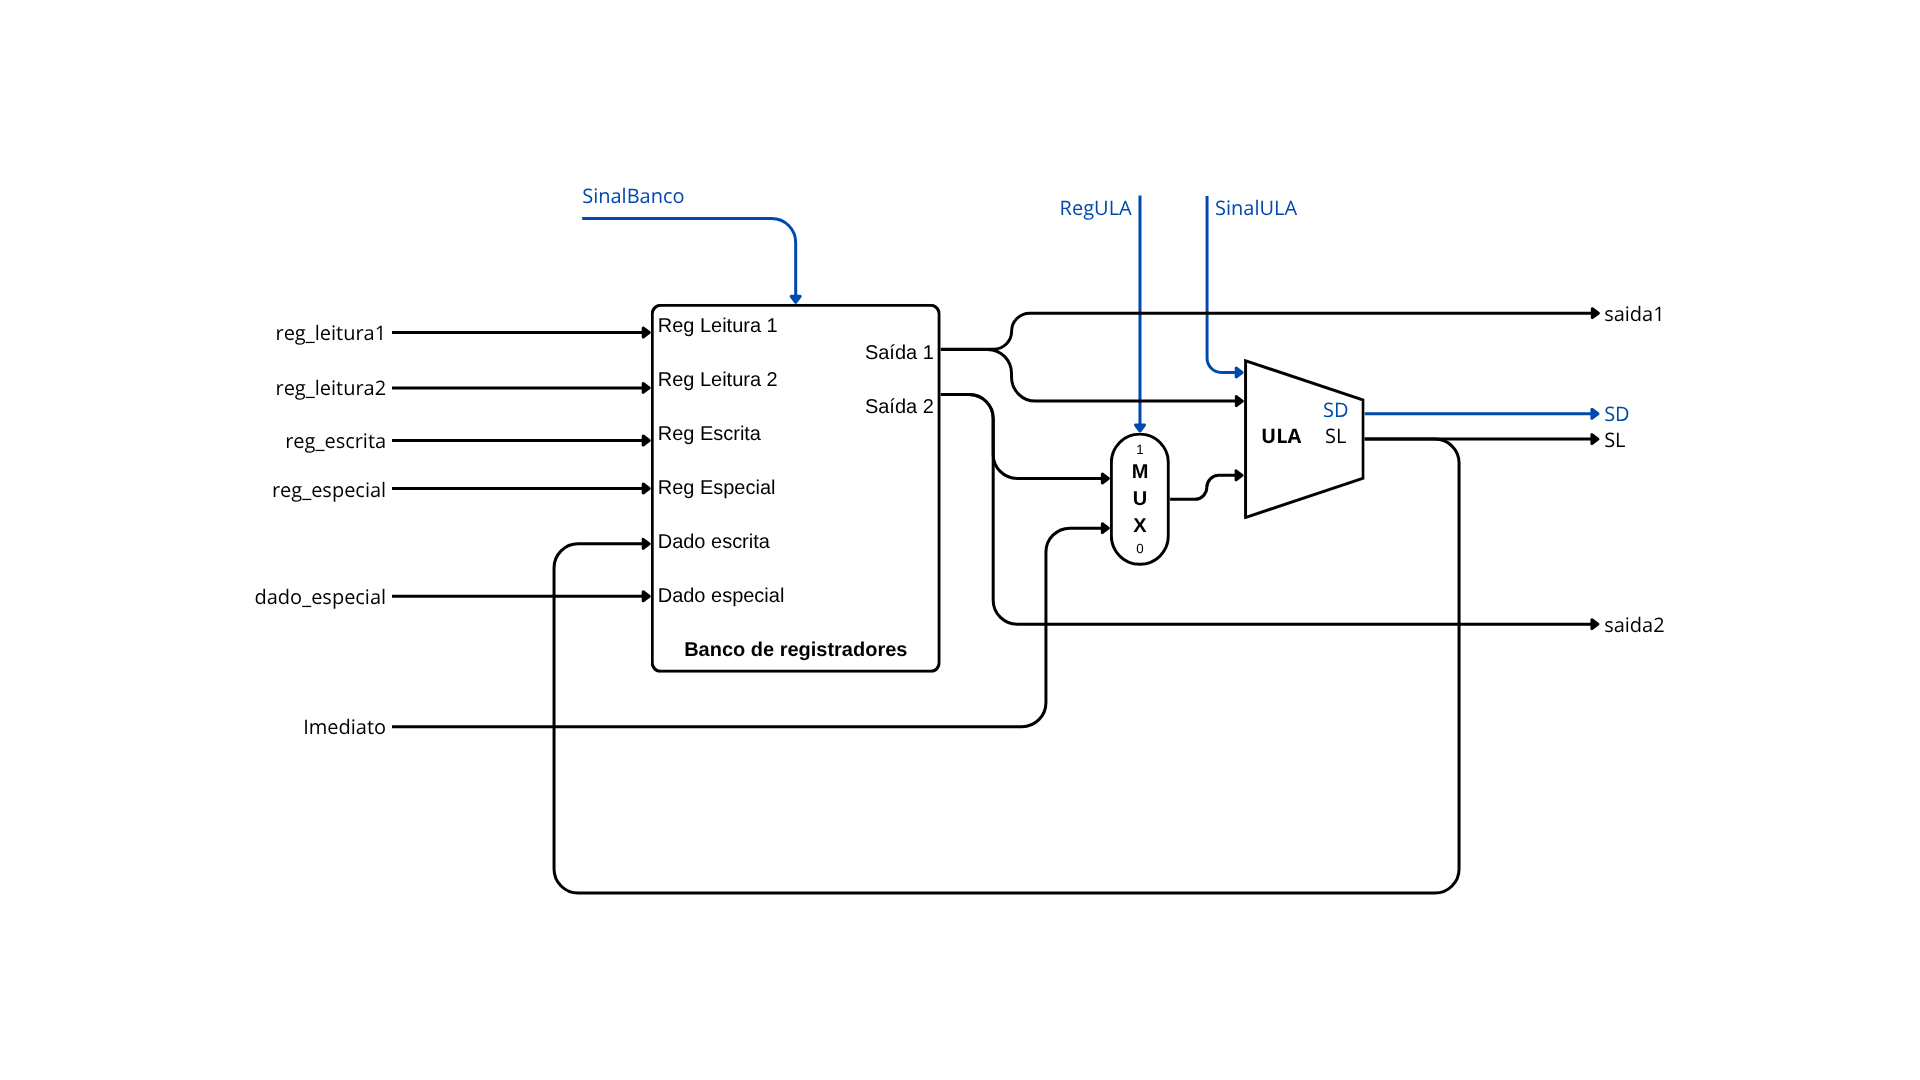
\includegraphics[width=0.7\textwidth]{Imagens/CmDados_Unidade_Processamento.png} \\
  Fonte: o Autor.
  \label{fig:cmdados_unidade_processamento}
\end{figure}

Como sinais de entrada e saída, foram utilizados quase todos os sinais usados no módulo da ULA e no módulo do banco de registradores, presentes na \autoref{tab:IO-ULA} e \autoref{tab:IO-banco_registradores}. 

As entradas não utilizadas presentes na \autoref{tab:IO-ULA} são a EA e EB, pois os valores desses campos vêm da leitura do banco e do imediato. Além disso, não foi utilizada a entrada dado\_escrita da \autoref{tab:IO-banco_registradores}, pois os valores desses campos são providos diretamente da saída da ULA. Todos os sinais de saída foram usados.

Além disso, todos os sinais utilizados neste módulo se comportam da mesma forma que estão descritos na \autoref{tab:IO-ULA} e \autoref{tab:IO-banco_registradores}.

\subsection{Memória principal}

A memória principal, também chamada de memória de dados, é responsável por armazenar o valor de variáveis durante a execução dos códigos, além de conter a pilha do processador. Os sinais de entrada e saída deste módulo estão presentes na \autoref{tab:IO_memoria_dados} abaixo.

\setlength{\tabcolsep}{10pt} % Define o tamanho das colunas
\begin{table}[H]
\centering
\caption{Entradas e saídas do módulo da memória principal}
\label{tab:IO_memoria_dados}
\begin{tabular}{|c|c|l|}
\hline
\multicolumn{3}{|c|}{\textbf{ENTRADAS}} \\
\hline
\textbf{Sinal} & \textbf{Nº bits} & \textbf{Descrição} \\
\hline
clock & 1 & Controla a escrita, feita somente na borda de subida \\
\hline
END & 6 & Endereço com a posição da memória a ser acessada \\
\hline
dado\_escrita & 32 & Valor a ser escrito no endereço \\
\hline
SinalMemoria & 1 & Controla a escrita no endereço (1=sim, 0=não) \\
\hline
\multicolumn{3}{|c|}{\textbf{SAÍDAS}} \\
\hline
\textbf{Sinal} & \textbf{Nº bits} & \textbf{Descrição} \\
\hline
saida & 32 & Valor lido no endereço \\
\hline
\end{tabular}
\vspace{-0.5em}
\begin{center}
Fonte: o Autor.
\end{center}
\end{table}

Note que a escrita ocorre somente na borda de subida do clock e se o valor de SinalMemoria for 1. Por outro lado, a leitura é feita de modo assíncrono, com a saída sendo dada pelo valor no endereço.

Além disso, a memória principal foi criada como uma matriz de 64 linhas de 32 bits. A princípio, foi escolhido o valor de 64 linhas para testar, pois o tempo de compilação não é muito longo. Os 32 bits é devido ao tamanho dos registradores que são de 32 bits cada um.

\subsection{Memória de instruções}

A memória de instruções contém os códigos a serem executados pelo processador. As entradas e saídas desse módulo estão na \autoref{tab:IO_memoria_instrucoes} abaixo.

\setlength{\tabcolsep}{10pt} % Define o tamanho das colunas
\begin{table}[H]
\centering
\caption{Entradas e saídas do módulo da memória de instruções}
\label{tab:IO_memoria_instrucoes}
\begin{tabular}{|c|c|l|}
\hline
\multicolumn{3}{|c|}{\textbf{ENTRADAS}} \\
\hline
\textbf{Sinal} & \textbf{Nº bits} & \textbf{Descrição} \\
\hline
clock & 1 & Controla a saída, atualizada na borda de descida \\
\hline
PC & 6 & Endereço com a posição da memória a ser acessada \\
\hline
\multicolumn{3}{|c|}{\textbf{SAÍDAS}} \\
\hline
\textbf{Sinal} & \textbf{Nº bits} & \textbf{Descrição} \\
\hline
Opcode & 6 & Opcode da instrução lida na memória \\
\hline
Operandos & 26 & A instrução sem o Opcode \\
\hline
\end{tabular}
\vspace{-0.5em}
\begin{center}
Fonte: o Autor.
\end{center}
\end{table} 

Primeiramente, o valor da saída é atualizado somente na borda de descida do clock. Isso é feito para garantir o funcionamento correto do processador, para que seja possível, nos demais módulos, processar a instrução e realizar as escritas na borda de subida do clock.

Além disso, a saída é dividida em dois campos: Opcode e Operandos. Isso é feito pois o Opcode será enviado diretamente para a unidade de controle, enquanto a saída com os operandos será enviada para o gerenciador de entrada.

Ademais, as instruções são lidas de um arquivo chamado ``single\_port\_rom\_init.txt'', sendo assim, elas não são passadas diretamente pelo código em Verilog. Esse arquivo deve conter uma instrução por linha e todas as instruções devem ter 32 bits.

Além disso, foi tomado o valor do Opcode no instante inicial como sendo 000001, de modo a garantir que não seja executada uma instrução inválida ao iniciar o processador. Esse Opcode em questão corresponde à instrução nop, portanto, nada será executado, apenas passará um ciclo de clock.

\subsection{PC}

O módulo do PC controla o endereço da instrução a ser lida na memória de instruções. Para isso, ele atualiza o valor do PC de acordo com o novo valor que ele deve receber. Os sinais de entrada e saída estão presentes na \autoref{tab:IO_PC} abaixo.

\setlength{\tabcolsep}{10pt} % Define o tamanho das colunas
\begin{table}[H]
\centering
\caption{Entradas e saídas do módulo PC}
\label{tab:IO_PC}
\begin{tabular}{|c|c|l|}
\hline
\multicolumn{3}{|c|}{\textbf{ENTRADAS}} \\
\hline
\textbf{Sinal} & \textbf{Nº bits} & \textbf{Descrição} \\
\hline
clock & 1 & Controla a saída, atualizada na borda de subida \\
\hline
Novo\_Endereco & 6 & Endereço o novo valor do PC \\
\hline
HLT & 1 & Impede a atualização do PC (1=sim, 0=não)\\
\hline
TravaPC & 1 & \makecell[l]{Impede o PC atualizar até um botão ser pressionado \\ (1=sim, 0=não)} \\
\hline
\multicolumn{3}{|c|}{\textbf{SAÍDAS}} \\
\hline
\textbf{Sinal} & \textbf{Nº bits} & \textbf{Descrição} \\
\hline
PC & 6 & Saída com o novo valor do PC \\
\hline
\end{tabular}
\vspace{-0.5em}
\begin{center}
Fonte: o Autor.
\end{center}
\end{table} 

A atualização do endereço do PC ocorre sempre na borda de descida do clock e somente se os valores tanto de HLT quanto de TravaPC forem baixos. O sinal HLT provém da unidade de controle e é gerado pela instrução de mesmo nome que interrompe o processador. Enquanto TravaPC é um sinal de controle enviado pelo módulo de entrada e saída enquanto ele espera que um valor seja inserido nos switches.

Após assumir o valor 1, o sinal HLT não pode voltar a ser zero, a não ser que o processador seja resetado. Por outro lado, o TravaPC é desativado quando um botão for pressionado, indicando que já foi colocado o valor desejado nos switches, então, eles são lidos e o código continua.

\subsection{Unidade de controle}

O papel da unidade de controle é, a partir dos Opcodes das instruções, determinar qual deve ser o sinal de controle para cada um dos sinais de controle. Isso é feito utilizando um case para cada uma das instruções e definindo qual deve ser o valor de cada sinal de controle para essa instrução funcionar corretamente.

A \autoref{tab:IO_unidade_controle} apresenta todos os sinais de entrada e saída que a unidade de controle utiliza, bem como o número de bits de cada um e a sua descrição. Nela o ``X'' indica que a respectiva escrita ocorre independente do sinal do outro bit.

\setlength{\tabcolsep}{10pt} % Define o tamanho das colunas
\begin{table}[H]
\centering
\caption{Entradas e saídas da unidade de controle}
\label{tab:IO_unidade_controle}
\begin{tabular}{|c|c|l|}
\hline
\multicolumn{3}{|c|}{\textbf{ENTRADAS}} \\
\hline
\textbf{Sinal} & \textbf{Nº bits} & \textbf{Descrição} \\
\hline
Opcode & 6 & Valor do Opcode da instrução \\
\hline
\multicolumn{3}{|c|}{\textbf{SAÍDAS}} \\
\hline
\textbf{Sinal} & \textbf{Nº bits} & \textbf{Descrição} \\
\hline
HLT & 1 & Impede o PC de atualizar \\
\hline
RegULA & 1 & Escolhe entre imediato [0] e registrador [1] para ULA \\
\hline
SinalMemoria & 1 & Indica escrita na memória de dados \\
\hline
SinalMES & 2 & Indica se é uma instrução IN [01] ou OUT [10]\\
\hline
SinalBanco & 2 & Controla escrita [X1] e escrita especial [1X] \\
\hline
SinalMuxE & 2 & Define qual será o dado de escrita \\
\hline
SinalMuxEE & 2 & Define qual será o dado de escrita especial \\
\hline
SinalMuxPC & 2 & Define o próximo valor do PC \\
\hline
SinalGEN & 3 & Define como serão obtido os operando da instrução \\
\hline
SinalULA & 5 & Operação a ser realizada pela ULA \\
\hline
\end{tabular}
\vspace{-0.5em}
\begin{center}
Fonte: o Autor.
\end{center}
\end{table} 



\subsection{Módulo de entrada e saída}

O módulo de entrada e saída é responsável por receber os valores lidos pelos switches e enviá-los para o mux de escrita. Durante a leitura, o módulo também é responsável pelo sinal de controle TravaPC, responsável por parar a atualização do PC até que um botão de controle seja pressionado, indicando que foi escrito o valor desejado nos switches.

Além do mais, também é responsável por receber um registrador que deve ter o seu conteúdo lido. Para isso, implementa um decodificador que, a partir de um valor em binário de 32 bits, identifica quais são cada um dos dígitos desse valor ao ser convertido para decimal. Ademais, a partir desses dígitos em decimal, escreve em cada um dos oito displays de sete segmentos.

A \autoref{tab:IO_Entrada_E_Saida} apresenta os sinais de entrada e saída do módulo de entrada e saída, bem como o número de bits de cada um e a descrição. Nela o ``Display\_X'' foi escrito dessa forma pois, ao todo, há 8 displays e, para cada um deles, há um sinal de saída. Desse modo, foi usado ``X'' para indicar cada uma dessas 8 possibilidades.

\setlength{\tabcolsep}{10pt} % Define o tamanho das colunas
\begin{table}[H]
\centering
\caption{Entradas e saídas do módulo de entrada e saída}
\label{tab:IO_Entrada_E_Saida}
\begin{tabular}{|c|c|l|}
\hline
\multicolumn{3}{|c|}{\textbf{ENTRADAS}} \\
\hline
\textbf{Sinal} & \textbf{Nº bits} & \textbf{Descrição} \\
\hline
clock & 1 & Sinal de clock \\
\hline
SinalMES & 2 & Controla a leitura (bit 0) e a escrita (bit 1)\\
\hline
Display\_IN & 32 & Valor a ser escrito no display \\
\hline
Switches\_IN & 18 & Valor lido dos 18 switches\\
\hline
Destrava & 1 & Botão que destrava o PC \\
\hline
\multicolumn{3}{|c|}{\textbf{SAÍDAS}} \\
\hline
\textbf{Sinal} & \textbf{Nº bits} & \textbf{Descrição} \\
\hline
Switches\_OUT & 32 & Valor dos switches extendido \\
\hline
TravaPC & 1 & Sinal que impede o PC de atualizar \\
\hline
Display\_X & 7 & Valor a ser escrito no display X \\
\hline
\end{tabular}
\vspace{-0.5em}
\begin{center}
Fonte: o Autor.
\end{center}
\end{table} 

Nesse módulo o sinal TravaPC se torna 1 sempre que é executada uma instrução IN. Além disso, permanece como 1 até que seja pressionado o botão destrava.

Para o funcionamento correto do botão, foi necessário implementar um debouncer para garantir que o TravaPC só volte a ser zero uma única vez a cada vez que o botão for pressionado. Isso foi necessário pois, caso contrário, um único pulso no botão poderia tomar a mesma configuração de switches como sinal de entrada para várias instruções IN em sequência.

Além disso, dentro do módulo também foi criado um buffer para que o valor escrito no display só seja atualizado nas instruções OUT e, nas demais instruções, permaneça com seu valor inalterado.

Ademais, no mesmo documento em que foi desenvolvido o módulo de entrada e saída, também foi criado um módulo para converter dígitos de binário para o display de sete segmentos por meio de um case.

\subsection{Integração final}

A integração final tem o papel de unir o conteúdo de todos os módulos desenvolvidos de modo que sejam capazes de se comunicarem entre si e, dessa forma, simular o comportamento de um processador usando a linguagem Verilog.

Para isso, foi necessário criar um arquivo em Verilog e, a partir dele, chamar a todos os outros módulos desenvolvidos, passando as respectivas variáveis de entrada e saída para cada um deles.

A \autoref{tab:IO_Integração_Final} apresenta os sinais de entrada e saída da integração final de todos os módulos, bem como o número de bits de cada um e a descrição. Nela, de modo similar aos sinais de saída do módulo de entrada e saída, o sinal ``Display\_X'' foi escrito dessa forma com o ``X'' representando os 8 displays.

\setlength{\tabcolsep}{10pt} % Define o tamanho das colunas
\begin{table}[H]
\centering
\caption{Entradas e saídas da integração final}
\label{tab:IO_Integração_Final}
\begin{tabular}{|c|c|l|}
\hline
\multicolumn{3}{|c|}{\textbf{ENTRADAS}} \\
\hline
\textbf{Sinal} & \textbf{Nº bits} & \textbf{Descrição} \\
\hline
clock & 1 & Sinal de clock do FPGA 50MHz\\
\hline
Destrava & 1 & Botão para destravar o PC \\
\hline
Switches\_IN & 18 & Valor de entrada dos 18 switches \\
\hline
\multicolumn{3}{|c|}{\textbf{SAÍDAS}} \\
\hline
\textbf{Sinal} & \textbf{Nº bits} & \textbf{Descrição} \\
\hline
Display\_X & 7 & Valor a ser escrito no display X \\
\hline
\end{tabular}
\vspace{-0.5em}
\begin{center}
Fonte: o Autor.
\end{center}
\end{table} 

Nesse módulo também foi desenvolvido um divisor de frequência de 50MHz para 1MHz, com somente esse sinal com a frequência reduzida sendo passado para os demais módulos.

% ---------------------------------------------------------
% ---------------------------------------------------------
% ---------------------------------------------------------

\section{Implementações}

\subsection{ULA}

No \autoref{cod:ULA_verilog} abaixo é apresentado o código desenvolvido para a ULA.

\begin{lstlisting}[language=Verilog, caption={Módulo da ULA em Verilog}, label={cod:ULA_verilog}]
module ULA (
    input wire [31:0] EA,
    input wire [31:0] EB,
    input wire [4:0] SinalULA,
    output reg [31:0] SL,
    output reg SD
);

// Atribuicao inicial para evitar latches (logica combinacional pura)
always @(*) begin
    SL = 32'd0;
    SD = 1'b0;

    case(SinalULA)
        5'b00000: SL = EA + EB;
        5'b00001: SL = EA - EB;
        5'b00010: SL = EA & EB;
        5'b00011: SL = EA | EB;
        5'b00100: SL = ~EA;
        5'b00101: SL = EA ~^ EB;
        5'b00110: SL = EA << EB[4:0];
        5'b00111: SL = EA >> EB[4:0];
        5'b01000: SD = (EA == EB);
        5'b01001: SD = (EA != EB);
        5'b01010: SD = (EA < EB);
        5'b01011: SD = (EA > EB);
        5'b01100: SL = EA * EB;
        5'b01101: SL = EA / EB;
        5'b01110: SL = EA;
        5'b01111: SL = EB;
        5'b10000: SL = EA + 1;
        5'b10001: SD = (EA <= EB);
        5'b10010:  SD = (EA >= EB);
        default: begin
            SL = 32'd0;
            SD = 1'b0;
        end
    endcase
end

endmodule

\end{lstlisting}

\newpage

\subsection{Banco de registradores}

No \autoref{cod:banco_reistradores_verilog} abaixo é apresentado o código desenvolvido para o banco de registradores.

\begin{lstlisting}[language=Verilog, caption={Módulo do banco de registradores em Verilog}, label={cod:banco_reistradores_verilog}]
module Banco_de_Registradores
#(parameter ADDR_WIDTH = 6)			// 2^4 = 16 registradores (mude para 5 para 32, ou 6 para 64)
(clock, reg_leitura1, reg_leitura2, reg_escrita, reg_especial, dado_escrita, dado_especial, SinalBanco, saida1, saida2);

input clock;								// Clock do processador
input [5:0] reg_leitura1;				// Endereco do registrador 1
input [5:0] reg_leitura2;				// Endereco do registrador 2
input [5:0] reg_escrita;				// Endereco de escrita
input [5:0] reg_especial;				// Endereco de escrita especial
input [31:0] dado_escrita;				// Dado para escrever
input [31:0] dado_especial;			// Dado para escrever especial

input [1:0] SinalBanco;					// [00] = sem escrita, [01] = escrita padrao, [10] = escrita especial, [11] = ambos

output [31:0] saida1;					// Dado de saida 1
output [31:0] saida2;					// Dado de saida 2

reg [31:0] banco [2**ADDR_WIDTH-1:0];				// Criacao do banco de registradores

always @(posedge clock)
begin
    // Garante que o registrador 0 (6'd0) nunca seja sobrescrito
    if(SinalBanco[0] == 1'b1 && reg_escrita[ADDR_WIDTH-1:0] != 0) 
        banco[reg_escrita[ADDR_WIDTH-1:0]] <= dado_escrita;
        
    if(SinalBanco[1] == 1'b1 && reg_especial[ADDR_WIDTH-1:0] != 0) 
        banco[reg_especial[ADDR_WIDTH-1:0]] <= dado_especial;
end

// Se a leitura for no Endereco 0, a saida e 0. Caso contrario, le o banco normalmente.
assign saida1 = (reg_leitura1[ADDR_WIDTH-1:0] == 0) ? 32'd0 : banco[reg_leitura1[ADDR_WIDTH-1:0]];
assign saida2 = (reg_leitura2[ADDR_WIDTH-1:0] == 0) ? 32'd0 : banco[reg_leitura2[ADDR_WIDTH-1:0]];
	
endmodule
\end{lstlisting}

\newpage

\subsection{Integração ULA com banco de registradores}

No \autoref{cod:integracao_ULA_banco_verilog} abaixo é apresentado o código desenvolvido para a integração da ULA com o banco de registradores.

\begin{lstlisting}[language=Verilog, caption={Módulo da integração da ULA com o banco de registradores em Verilog}, label={cod:integracao_ULA_banco_verilog}]
module Integracao_ULA_Banco (
// Entradas e saidas para o banco
input clock,					        // Clock do processador
input [5:0] reg_leitura1,				// Endereco do registrador 1
input [5:0] reg_leitura2,				// Endereco do registrador 2
input [5:0] reg_escrita,				// Endereco de escrita
input [5:0] reg_especial,				// Endereco de escrita especial
input [31:0] dado_especial,			        // Dado para escrever especial
input [1:0] SinalBanco,					// Controla a escrita: bit[1] = especial, bit[0] = escrita
output [31:0] saida1,					// Valor do primeiro registrador lido
output [31:0] saida2,					// Valor do segundo registrador lido

// Entradas e saidas para ULA
input [4:0] SinalULA,					// Codigo de operacao da ULA
output [31:0] SL,					// Saida padrao
output SD,						// Saida para desvio

// Entrada de imediato
input [31:0] Imediato,					// Imediato
input RegULA				                // Sinal que define se e imediato (0) ou reg (1)
);

wire [31:0] EA;
wire [31:0] EB;

// Envia os dados para o banco
Banco_de_Registradores #(.ADDR_WIDTH(6)) banco_inst (
	.clock(clock), 	
	.reg_leitura1(reg_leitura1), 
	.reg_leitura2(reg_leitura2), 
	.reg_escrita(reg_escrita), 
	.reg_especial(reg_especial), 
	.dado_escrita(SL), 				// Saida padrao da ULA
	.dado_especial(dado_especial), 
	.SinalBanco(SinalBanco), 
	.saida1(saida1), 
	.saida2(saida2)
);

// Atribui os valores de entrada para ULA
// Primeira entreada da ULA vem da saida1 do banco
assign EA = saida1; 

// Segunda entrada vem ou da saida2 ou do imediato
Mux2(
	.E1(saida2), 
	.E2(Imediato), 
	.S(EB), 
	.Sinal(RegULA)
);

// Envia os dados para ULA
ULA(
	.EA(EA), 
	.EB(EB), 
	.SinalULA(SinalULA), 
	.SL(SL), 
	.SD(SD)
);

endmodule 
\end{lstlisting}

\newpage

\subsection{Memória principal}

No \autoref{cod:memoria_principal_verilog} abaixo é apresentado o código desenvolvido para a memória principal.

\begin{lstlisting}[language=Verilog, caption={Módulo da memória principal em Verilog}, label={cod:memoria_principal_verilog}]
// Quartus Prime Verilog Template

module Memoria_Principal
#(parameter DATA_WIDTH=32, parameter ADDR_WIDTH=8) // 32 bits e 2^8 = 256 linhas
(
	input clock,										// Sinal de clock
	input [(ADDR_WIDTH-1):0] END,	  				// Endereco de acesso
	input [(DATA_WIDTH-1):0] dado_escrita,		// Dado para escrever
	input SinalMemoria, 								// Sinal de escrita
	output reg [(DATA_WIDTH-1):0] saida			// Dado de saida				
);
	
	// Criacao da memoria
	reg [DATA_WIDTH-1:0] ram[2**ADDR_WIDTH-1:0];
	
	always @ (negedge clock)
	begin
		// Escrita na memoria
		if (SinalMemoria) ram[END] <= dado_escrita;
		
		// Leitura
		saida <= ram[END];
	end
	
endmodule
\end{lstlisting}

\newpage

\subsection{Memória instruções}

No \autoref{cod:memoria_instrucoes_verilog} abaixo é apresentado o código desenvolvido para a memória de instruções.

\begin{lstlisting}[language=Verilog, caption={Módulo da memória de instruções em Verilog}, label={cod:memoria_instrucoes_verilog}]
// Quartus Prime Verilog Template
// Single Port ROM

module Memoria_Instrucoes
#(parameter DATA_WIDTH=32, parameter ADDR_WIDTH=8)
( 
	input clock,
	input [(ADDR_WIDTH-1):0] PC,
	output reg [5:0] Opcode,
	output reg [25:0] Operandos
);

	// Declare the ROM variable
	reg [DATA_WIDTH-1:0] rom[2**ADDR_WIDTH-1:0];

	// Initialize the ROM with $readmemb.  Put the memory contents
	// in the file single_port_rom_init.txt.  Without this file,
	// this design will not compile.

	// See Verilog LRM 1364-2001 Section 17.2.8 for details on the
	// format of this file, or see the "Using $readmemb and $readmemh"
	// template later in this section.

	initial 
	begin
		$readmemb("single_port_rom_init.txt", rom);
		Opcode = 6'd1;       // Forca Opcode inicial como 000001 (nop)
		Operandos = 26'd0;   // Apenas para atribuir um valor
	end


	always @ (posedge clock)
	begin
		Opcode <= rom[PC][31:26];
		Operandos <= rom[PC][25:0];
	end

endmodule
\end{lstlisting}

\newpage

\subsection{PC}

No \autoref{cod:PC_verilog} abaixo é apresentado o código desenvolvido para o módulo do PC.

\begin{lstlisting}[language=Verilog, caption={Módulo do PC em Verilog}, label={cod:PC_verilog}]
module PC(clock, Novo_Endereco, HLT, TravaPC, PC);

input clock;						// Sinal de clock
input [7:0]Novo_Endereco;		// Novo valor do PC
input HLT;							// Sinal de encerrar
input TravaPC;						// Sinal para segurar para ler switches
output reg [7:0]PC;				// Saida do PC

reg aux = 1'b0;

always @(negedge clock)
begin
	if(aux == 1'b0)
	begin
		PC = 7'd0;
		aux = 1'b1;
	end

	if(!HLT & !TravaPC)
	begin
		PC = Novo_Endereco;
	end
end

endmodule 
\end{lstlisting}

\newpage

\subsection{Unidade de controle}

No \autoref{cod:unidade_de_controle_verilog} abaixo é apresentado o código desenvolvido para o módulo da unidade de controle.

\begin{lstlisting}[language=Verilog, caption={Módulo da unidade de controle em Verilog}, label={cod:unidade_de_controle_verilog}]
module Unidade_de_Controle(
input [5:0] Opcode,
output reg HLT,
output reg RegULA,
output reg SinalMemoria,
output reg [1:0] SinalMES,
output reg [1:0] SinalBanco,
output reg [1:0] SinalMuxE,
output reg [1:0] SinalMuxEE,
output reg [1:0] SinalMuxPC,
output reg [2:0] SinalGEN,
output reg [4:0] SinalULA
);

always @(*)
begin
	SinalMES = 2'b00;
			
	case(Opcode)
		// Formato 7 - hlt
		6'b000000:
		begin
			HLT = 1'b1;
			RegULA = 1'b0; 			// Registrador para ULA
			SinalMemoria = 1'b0; 	// Controla escrita
			SinalMES = 2'b00;       // [10] = OUT, [01] = IN, [00] = default
			SinalBanco = 2'b00; 		// [00] = sem escrita, [01] = escrita padrao, [10] = escrita especial, [11] = ambos
			SinalMuxE = 2'b00; 		// [00] = Switches, [01] = ULA, [10] = Memoria
			SinalMuxEE = 2'b00;  	// [00] = RAL, [01] = Push, [10] = Pop
			SinalMuxPC = 2'b00; 		// [00] = PC, [01] = J, [10] = Desvio, [11] = JR
			SinalGEN = 3'b110; 		// Num Formato - 1
			SinalULA = 5'b11111; 
		end
		// Formato 7 - nop
		6'b000001:
		begin
			HLT = 1'b0;
			RegULA = 1'b0; 			// Registrador para ULA
			SinalMemoria = 1'b0; 	// Controla escrita
			SinalMES = 2'b00;       // [10] = OUT, [01] = IN, [00] = default
			SinalBanco = 2'b00; 		// [00] = sem escrita, [01] = escrita padrao, [10] = escrita especial, [11] = ambos
			SinalMuxE = 2'b00; 		// [00] = Switches, [01] = ULA, [10] = Memoria
			SinalMuxEE = 2'b00;  	// [00] = RAL, [01] = Push, [10] = Pop
			SinalMuxPC = 2'b00; 		// [00] = PC, [01] = J, [10] = Desvio, [11] = JR
			SinalGEN = 3'b110; 		// Num Formato - 1
			SinalULA = 5'b11111; 
		end
		// Formato 7 - jmp
		6'b000010:
		begin
			HLT = 1'b0;
			RegULA = 1'b0; 			// Registrador para ULA
			SinalMemoria = 1'b0; 	// Controla escrita
			SinalMES = 2'b00;       // [10] = OUT, [01] = IN, [00] = default
			SinalBanco = 2'b00; 		// [00] = sem escrita, [01] = escrita padrao, [10] = escrita especial, [11] = ambos
			SinalMuxE = 2'b00; 		// [00] = Switches, [01] = ULA, [10] = Memoria
			SinalMuxEE = 2'b00;  	// [00] = RAL, [01] = Push, [10] = Pop
			SinalMuxPC = 2'b01; 		// [00] = PC, [01] = J, [10] = Desvio, [11] = JR
			SinalGEN = 3'b110; 		// Num Formato - 1
			SinalULA = 5'b11111; 
		end
		// Formato 7 - jal
		6'b000011:
		begin
			HLT = 1'b0;
			RegULA = 1'b0; 			// Registrador para ULA
			SinalMemoria = 1'b0; 	// Controla escrita
			SinalMES = 2'b00;       // [10] = OUT, [01] = IN, [00] = default
			SinalBanco = 2'b10; 		// [00] = sem escrita, [01] = escrita padrao, [10] = escrita especial, [11] = ambos
			SinalMuxE = 2'b00; 		// [00] = Switches, [01] = ULA, [10] = Memoria
			SinalMuxEE = 2'b00;  	// [00] = RAL, [01] = Push, [10] = Pop
			SinalMuxPC = 2'b01; 		// [00] = PC, [01] = J, [10] = Desvio, [11] = JR
			SinalGEN = 3'b110; 		// Num Formato - 1
			SinalULA = 5'b11111; 
		end
		// Formato 1 - add
		6'b000100:
		begin
			HLT = 1'b0;
			RegULA = 1'b1; 			// Registrador para ULA
			SinalMemoria = 1'b0; 	// Controla escrita
			SinalMES = 2'b00;       // [10] = OUT, [01] = IN, [00] = default
			SinalBanco = 2'b01; 		// [00] = sem escrita, [01] = escrita padrao, [10] = escrita especial, [11] = ambos
			SinalMuxE = 2'b01; 		// [00] = Switches, [01] = ULA, [10] = Memoria
			SinalMuxEE = 2'b00;  	// [00] = RAL, [01] = Push, [10] = Pop
			SinalMuxPC = 2'b00; 		// [00] = PC, [01] = J, [10] = Desvio, [11] = JR
			SinalGEN = 3'b000; 		// Num Formato - 1
			SinalULA = 5'b00000; 
		end
		// Formato 1 - sub
		6'b000101:
		begin
			HLT = 1'b0;
			RegULA = 1'b1; 			// Registrador para ULA
			SinalMemoria = 1'b0; 	// Controla escrita
			SinalMES = 2'b00;       // [10] = OUT, [01] = IN, [00] = default
			SinalBanco = 2'b01; 		// [00] = sem escrita, [01] = escrita padrao, [10] = escrita especial, [11] = ambos
			SinalMuxE = 2'b01; 		// [00] = Switches, [01] = ULA, [10] = Memoria
			SinalMuxEE = 2'b00;  	// [00] = RAL, [01] = Push, [10] = Pop
			SinalMuxPC = 2'b00; 		// [00] = PC, [01] = J, [10] = Desvio, [11] = JR
			SinalGEN = 3'b000; 		// Num Formato - 1
			SinalULA = 5'b00001; 
		end
		// Formato 1 - mul
		6'b000110:
		begin
			HLT = 1'b0;
			RegULA = 1'b1; 			// Registrador para ULA
			SinalMemoria = 1'b0; 	// Controla escrita
			SinalMES = 2'b00;       // [10] = OUT, [01] = IN, [00] = default
			SinalBanco = 2'b01; 		// [00] = sem escrita, [01] = escrita padrao, [10] = escrita especial, [11] = ambos
			SinalMuxE = 2'b01; 		// [00] = Switches, [01] = ULA, [10] = Memoria
			SinalMuxEE = 2'b00;  	// [00] = RAL, [01] = Push, [10] = Pop
			SinalMuxPC = 2'b00; 		// [00] = PC, [01] = J, [10] = Desvio, [11] = JR
			SinalGEN = 3'b000; 		// Num Formato - 1
			SinalULA = 5'b01100; 
		end
		// Formato 1 - div
		6'b000111:
		begin
			HLT = 1'b0;
			RegULA = 1'b1; 			// Registrador para ULA
			SinalMemoria = 1'b0; 	// Controla escrita
			SinalMES = 2'b00;       // [10] = OUT, [01] = IN, [00] = default
			SinalBanco = 2'b01; 		// [00] = sem escrita, [01] = escrita padrao, [10] = escrita especial, [11] = ambos
			SinalMuxE = 2'b01; 		// [00] = Switches, [01] = ULA, [10] = Memoria
			SinalMuxEE = 2'b00;  	// [00] = RAL, [01] = Push, [10] = Pop
			SinalMuxPC = 2'b00; 		// [00] = PC, [01] = J, [10] = Desvio, [11] = JR
			SinalGEN = 3'b000; 		// Num Formato - 1
			SinalULA = 5'b01101; 
		end
		// Formato 1 - and
		6'b001000:
		begin
			HLT = 1'b0;
			RegULA = 1'b1; 			// Registrador para ULA
			SinalMemoria = 1'b0; 	// Controla escrita
			SinalMES = 2'b00;       // [10] = OUT, [01] = IN, [00] = default
			SinalBanco = 2'b01; 		// [00] = sem escrita, [01] = escrita padrao, [10] = escrita especial, [11] = ambos
			SinalMuxE = 2'b01; 		// [00] = Switches, [01] = ULA, [10] = Memoria
			SinalMuxEE = 2'b00;  	// [00] = RAL, [01] = Push, [10] = Pop
			SinalMuxPC = 2'b00; 		// [00] = PC, [01] = J, [10] = Desvio, [11] = JR
			SinalGEN = 3'b000; 		// Num Formato - 1
			SinalULA = 5'b00010; 
		end
		// Formato 1 - or
		6'b001001:
		begin
			HLT = 1'b0;
			RegULA = 1'b1; 			// Registrador para ULA
			SinalMemoria = 1'b0; 	// Controla escrita
			SinalMES = 2'b00;       // [10] = OUT, [01] = IN, [00] = default
			SinalBanco = 2'b01; 		// [00] = sem escrita, [01] = escrita padrao, [10] = escrita especial, [11] = ambos
			SinalMuxE = 2'b01; 		// [00] = Switches, [01] = ULA, [10] = Memoria
			SinalMuxEE = 2'b00;  	// [00] = RAL, [01] = Push, [10] = Pop
			SinalMuxPC = 2'b00; 		// [00] = PC, [01] = J, [10] = Desvio, [11] = JR
			SinalGEN = 3'b000; 		// Num Formato - 1
			SinalULA = 5'b00011; 
		end
		// Formato 1 - xnor
		6'b001010:
		begin
			HLT = 1'b0;
			RegULA = 1'b1; 			// Registrador para ULA
			SinalMemoria = 1'b0; 	// Controla escrita
			SinalMES = 2'b00;       // [10] = OUT, [01] = IN, [00] = default
			SinalBanco = 2'b01; 		// [00] = sem escrita, [01] = escrita padrao, [10] = escrita especial, [11] = ambos
			SinalMuxE = 2'b01; 		// [00] = Switches, [01] = ULA, [10] = Memoria
			SinalMuxEE = 2'b00;  	// [00] = RAL, [01] = Push, [10] = Pop
			SinalMuxPC = 2'b00; 		// [00] = PC, [01] = J, [10] = Desvio, [11] = JR
			SinalGEN = 3'b000; 		// Num Formato - 1
			SinalULA = 5'b00101; 
		end
		// Formato 2 - addi
		6'b001011:
		begin
			HLT = 1'b0;
			RegULA = 1'b0; 			// Registrador para ULA
			SinalMemoria = 1'b0; 	// Controla escrita
			SinalMES = 2'b00;       // [10] = OUT, [01] = IN, [00] = default
			SinalBanco = 2'b01; 		// [00] = sem escrita, [01] = escrita padrao, [10] = escrita especial, [11] = ambos
			SinalMuxE = 2'b01; 		// [00] = Switches, [01] = ULA, [10] = Memoria
			SinalMuxEE = 2'b00;  	// [00] = RAL, [01] = Push, [10] = Pop
			SinalMuxPC = 2'b00; 		// [00] = PC, [01] = J, [10] = Desvio, [11] = JR
			SinalGEN = 3'b001; 		// Num Formato - 1
			SinalULA = 5'b00000; 
		end
		// Formato 2 - subi
		6'b001100:
		begin
			HLT = 1'b0;
			RegULA = 1'b0; 			// Registrador para ULA
			SinalMemoria = 1'b0; 	// Controla escrita
			SinalMES = 2'b00;       // [10] = OUT, [01] = IN, [00] = default
			SinalBanco = 2'b01; 		// [00] = sem escrita, [01] = escrita padrao, [10] = escrita especial, [11] = ambos
			SinalMuxE = 2'b01; 		// [00] = Switches, [01] = ULA, [10] = Memoria
			SinalMuxEE = 2'b00;  	// [00] = RAL, [01] = Push, [10] = Pop
			SinalMuxPC = 2'b00; 		// [00] = PC, [01] = J, [10] = Desvio, [11] = JR
			SinalGEN = 3'b001; 		// Num Formato - 1
			SinalULA = 5'b00001; 
		end
		// Formato 2 - muli
		6'b001101:
		begin
			HLT = 1'b0;
			RegULA = 1'b0; 			// Registrador para ULA
			SinalMemoria = 1'b0; 	// Controla escrita
			SinalMES = 2'b00;       // [10] = OUT, [01] = IN, [00] = default
			SinalBanco = 2'b01; 		// [00] = sem escrita, [01] = escrita padrao, [10] = escrita especial, [11] = ambos
			SinalMuxE = 2'b01; 		// [00] = Switches, [01] = ULA, [10] = Memoria
			SinalMuxEE = 2'b00;  	// [00] = RAL, [01] = Push, [10] = Pop
			SinalMuxPC = 2'b00; 		// [00] = PC, [01] = J, [10] = Desvio, [11] = JR
			SinalGEN = 3'b001; 		// Num Formato - 1
			SinalULA = 5'b01100; 
		end
		// Formato 2 - divi
		6'b001110:
		begin
			HLT = 1'b0;
			RegULA = 1'b0; 			// Registrador para ULA
			SinalMemoria = 1'b0; 	// Controla escrita
			SinalMES = 2'b00;       // [10] = OUT, [01] = IN, [00] = default
			SinalBanco = 2'b01; 		// [00] = sem escrita, [01] = escrita padrao, [10] = escrita especial, [11] = ambos
			SinalMuxE = 2'b01; 		// [00] = Switches, [01] = ULA, [10] = Memoria
			SinalMuxEE = 2'b00;  	// [00] = RAL, [01] = Push, [10] = Pop
			SinalMuxPC = 2'b00; 		// [00] = PC, [01] = J, [10] = Desvio, [11] = JR
			SinalGEN = 3'b001; 		// Num Formato - 1
			SinalULA = 5'b01101; 
		end
		// Formato 2 - andi
		6'b001111:
		begin
			HLT = 1'b0;
			RegULA = 1'b0; 			// Registrador para ULA
			SinalMemoria = 1'b0; 	// Controla escrita
			SinalMES = 2'b00;       // [10] = OUT, [01] = IN, [00] = default
			SinalBanco = 2'b01; 		// [00] = sem escrita, [01] = escrita padrao, [10] = escrita especial, [11] = ambos
			SinalMuxE = 2'b01; 		// [00] = Switches, [01] = ULA, [10] = Memoria
			SinalMuxEE = 2'b00;  	// [00] = RAL, [01] = Push, [10] = Pop
			SinalMuxPC = 2'b00; 		// [00] = PC, [01] = J, [10] = Desvio, [11] = JR
			SinalGEN = 3'b001; 		// Num Formato - 1
			SinalULA = 5'b00010; 
		end
		// Formato 2 - ori
		6'b010000:
		begin
			HLT = 1'b0;
			RegULA = 1'b0; 			// Registrador para ULA
			SinalMemoria = 1'b0; 	// Controla escrita
			SinalMES = 2'b00;       // [10] = OUT, [01] = IN, [00] = default
			SinalBanco = 2'b01; 		// [00] = sem escrita, [01] = escrita padrao, [10] = escrita especial, [11] = ambos
			SinalMuxE = 2'b01; 		// [00] = Switches, [01] = ULA, [10] = Memoria
			SinalMuxEE = 2'b00;  	// [00] = RAL, [01] = Push, [10] = Pop
			SinalMuxPC = 2'b00; 		// [00] = PC, [01] = J, [10] = Desvio, [11] = JR
			SinalGEN = 3'b001; 		// Num Formato - 1
			SinalULA = 5'b00011; 
		end
		// Formato 2 - not
		6'b010001:
		begin
			HLT = 1'b0;
			RegULA = 1'b0; 			// Registrador para ULA
			SinalMemoria = 1'b0; 	// Controla escrita
			SinalMES = 2'b00;       // [10] = OUT, [01] = IN, [00] = default
			SinalBanco = 2'b01; 		// [00] = sem escrita, [01] = escrita padrao, [10] = escrita especial, [11] = ambos
			SinalMuxE = 2'b01; 		// [00] = Switches, [01] = ULA, [10] = Memoria
			SinalMuxEE = 2'b00;  	// [00] = RAL, [01] = Push, [10] = Pop
			SinalMuxPC = 2'b00; 		// [00] = PC, [01] = J, [10] = Desvio, [11] = JR
			SinalGEN = 3'b001; 		// Num Formato - 1
			SinalULA = 5'b00100; 
		end
		// Formato 2 - sl
		6'b010010:
		begin
			HLT = 1'b0;
			RegULA = 1'b0; 			// Registrador para ULA
			SinalMemoria = 1'b0; 	// Controla escrita
			SinalMES = 2'b00;       // [10] = OUT, [01] = IN, [00] = default
			SinalBanco = 2'b01; 		// [00] = sem escrita, [01] = escrita padrao, [10] = escrita especial, [11] = ambos
			SinalMuxE = 2'b01; 		// [00] = Switches, [01] = ULA, [10] = Memoria
			SinalMuxEE = 2'b00;  	// [00] = RAL, [01] = Push, [10] = Pop
			SinalMuxPC = 2'b00; 		// [00] = PC, [01] = J, [10] = Desvio, [11] = JR
			SinalGEN = 3'b001; 		// Num Formato - 1
			SinalULA = 5'b00110; 
		end
		// Formato 2 - sr
		6'b010011:
		begin
			HLT = 1'b0;
			RegULA = 1'b0; 			// Registrador para ULA
			SinalMemoria = 1'b0; 	// Controla escrita
			SinalMES = 2'b00;       // [10] = OUT, [01] = IN, [00] = default
			SinalBanco = 2'b01; 		// [00] = sem escrita, [01] = escrita padrao, [10] = escrita especial, [11] = ambos
			SinalMuxE = 2'b01; 		// [00] = Switches, [01] = ULA, [10] = Memoria
			SinalMuxEE = 2'b00;  	// [00] = RAL, [01] = Push, [10] = Pop
			SinalMuxPC = 2'b00; 		// [00] = PC, [01] = J, [10] = Desvio, [11] = JR
			SinalGEN = 3'b001; 		// Num Formato - 1
			SinalULA = 5'b00111; 
		end
		// Formato 2 - mov
		6'b010100:
		begin
			HLT = 1'b0;
			RegULA = 1'b0; 			// Registrador para ULA
			SinalMemoria = 1'b0; 	// Controla escrita
			SinalMES = 2'b00;       // [10] = OUT, [01] = IN, [00] = default
			SinalBanco = 2'b01; 		// [00] = sem escrita, [01] = escrita padrao, [10] = escrita especial, [11] = ambos
			SinalMuxE = 2'b01; 		// [00] = Switches, [01] = ULA, [10] = Memoria
			SinalMuxEE = 2'b00;  	// [00] = RAL, [01] = Push, [10] = Pop
			SinalMuxPC = 2'b00; 		// [00] = PC, [01] = J, [10] = Desvio, [11] = JR
			SinalGEN = 3'b001; 		// Num Formato - 1
			SinalULA = 5'b01110; 
		end
		// Formato 2 - loadd
		6'b010101:
		begin
			HLT = 1'b0;
			RegULA = 1'b0; 			// Registrador para ULA
			SinalMemoria = 1'b0; 	// Controla escrita
			SinalMES = 2'b00;       // [10] = OUT, [01] = IN, [00] = default
			SinalBanco = 2'b01; 		// [00] = sem escrita, [01] = escrita padrao, [10] = escrita especial, [11] = ambos
			SinalMuxE = 2'b10; 		// [00] = Switches, [01] = ULA, [10] = Memoria
			SinalMuxEE = 2'b00;  	// [00] = RAL, [01] = Push, [10] = Pop
			SinalMuxPC = 2'b00; 		// [00] = PC, [01] = J, [10] = Desvio, [11] = JR
			SinalGEN = 3'b001; 		// Num Formato - 1
			SinalULA = 5'b00000; 
		end
		// Formato 2 - loadr
		6'b010110:
		begin
			HLT = 1'b0;
			RegULA = 1'b0; 			// Registrador para ULA
			SinalMemoria = 1'b0; 	// Controla escrita
			SinalMES = 2'b00;       // [10] = OUT, [01] = IN, [00] = default
			SinalBanco = 2'b01; 		// [00] = sem escrita, [01] = escrita padrao, [10] = escrita especial, [11] = ambos
			SinalMuxE = 2'b10; 		// [00] = Switches, [01] = ULA, [10] = Memoria
			SinalMuxEE = 2'b00;  	// [00] = RAL, [01] = Push, [10] = Pop
			SinalMuxPC = 2'b00; 		// [00] = PC, [01] = J, [10] = Desvio, [11] = JR
			SinalGEN = 3'b001; 		// Num Formato - 1
			SinalULA = 5'b01110; 
		end
		// Formato 3 - beq
		6'b010111:
		begin
			HLT = 1'b0;
			RegULA = 1'b1; 			// Registrador para ULA
			SinalMemoria = 1'b0; 	// Controla escrita
			SinalMES = 2'b00;       // [10] = OUT, [01] = IN, [00] = default
			SinalBanco = 2'b00; 		// [00] = sem escrita, [01] = escrita padrao, [10] = escrita especial, [11] = ambos
			SinalMuxE = 2'b00; 		// [00] = Switches, [01] = ULA, [10] = Memoria
			SinalMuxEE = 2'b00;  	// [00] = RAL, [01] = Push, [10] = Pop
			SinalMuxPC = 2'b10; 		// [00] = PC, [01] = J, [10] = Desvio, [11] = JR
			SinalGEN = 3'b010; 		// Num Formato - 1
			SinalULA = 5'b01000; 
		end
		// Formato 3 - bnq
		6'b011000:
		begin
			HLT = 1'b0;
			RegULA = 1'b1; 			// Registrador para ULA
			SinalMemoria = 1'b0; 	// Controla escrita
			SinalMES = 2'b00;       // [10] = OUT, [01] = IN, [00] = default
			SinalBanco = 2'b00; 		// [00] = sem escrita, [01] = escrita padrao, [10] = escrita especial, [11] = ambos
			SinalMuxE = 2'b00; 		// [00] = Switches, [01] = ULA, [10] = Memoria
			SinalMuxEE = 2'b00;  	// [00] = RAL, [01] = Push, [10] = Pop
			SinalMuxPC = 2'b10; 		// [00] = PC, [01] = J, [10] = Desvio, [11] = JR
			SinalGEN = 3'b010; 		// Num Formato - 1
			SinalULA = 5'b01001; 
		end
		// Formato 3 - blt
		6'b011001:
		begin
			HLT = 1'b0;
			RegULA = 1'b1; 			// Registrador para ULA
			SinalMemoria = 1'b0; 	// Controla escrita
			SinalMES = 2'b00;       // [10] = OUT, [01] = IN, [00] = default
			SinalBanco = 2'b00; 		// [00] = sem escrita, [01] = escrita padrao, [10] = escrita especial, [11] = ambos
			SinalMuxE = 2'b00; 		// [00] = Switches, [01] = ULA, [10] = Memoria
			SinalMuxEE = 2'b00;  	// [00] = RAL, [01] = Push, [10] = Pop
			SinalMuxPC = 2'b10; 		// [00] = PC, [01] = J, [10] = Desvio, [11] = JR
			SinalGEN = 3'b010; 		// Num Formato - 1
			SinalULA = 5'b01010; 
		end
		// Formato 3 - bgt
		6'b011010:
		begin
			HLT = 1'b0;
			RegULA = 1'b1; 			// Registrador para ULA
			SinalMemoria = 1'b0; 	// Controla escrita
			SinalMES = 2'b00;       // [10] = OUT, [01] = IN, [00] = default
			SinalBanco = 2'b00; 		// [00] = sem escrita, [01] = escrita padrao, [10] = escrita especial, [11] = ambos
			SinalMuxE = 2'b00; 		// [00] = Switches, [01] = ULA, [10] = Memoria
			SinalMuxEE = 2'b00;  	// [00] = RAL, [01] = Push, [10] = Pop
			SinalMuxPC = 2'b10; 		// [00] = PC, [01] = J, [10] = Desvio, [11] = JR
			SinalGEN = 3'b010; 		// Num Formato - 1
			SinalULA = 5'b01011; 
		end
		// Formato 3 - stored
		6'b011011:
		begin
			HLT = 1'b0;
			RegULA = 1'b0; 			// Registrador para ULA
			SinalMemoria = 1'b1; 	// Controla escrita
			SinalMES = 2'b00;       // [10] = OUT, [01] = IN, [00] = default
			SinalBanco = 2'b00; 		// [00] = sem escrita, [01] = escrita padrao, [10] = escrita especial, [11] = ambos
			SinalMuxE = 2'b00; 		// [00] = Switches, [01] = ULA, [10] = Memoria
			SinalMuxEE = 2'b00;  	// [00] = RAL, [01] = Push, [10] = Pop
			SinalMuxPC = 2'b00; 		// [00] = PC, [01] = J, [10] = Desvio, [11] = JR
			SinalGEN = 3'b010; 		// Num Formato - 1
			SinalULA = 5'b00000; 
		end
		// Formato 3 - storer
		6'b011100:
		begin
			HLT = 1'b0;
			RegULA = 1'b0; 			// Registrador para ULA
			SinalMemoria = 1'b1; 	// Controla escrita
			SinalMES = 2'b00;       // [10] = OUT, [01] = IN, [00] = default
			SinalBanco = 2'b00; 		// [00] = sem escrita, [01] = escrita padrao, [10] = escrita especial, [11] = ambos
			SinalMuxE = 2'b00; 		// [00] = Switches, [01] = ULA, [10] = Memoria
			SinalMuxEE = 2'b00;  	// [00] = RAL, [01] = Push, [10] = Pop
			SinalMuxPC = 2'b00; 		// [00] = PC, [01] = J, [10] = Desvio, [11] = JR
			SinalGEN = 3'b010; 		// Num Formato - 1
			SinalULA = 5'b01110; 
		end
		// Formato 4 - movi
		6'b011101:
		begin
			HLT = 1'b0;
			RegULA = 1'b0; 			// Registrador para ULA
			SinalMemoria = 1'b0; 	// Controla escrita
			SinalMES = 2'b00;       // [10] = OUT, [01] = IN, [00] = default
			SinalBanco = 2'b01; 		// [00] = sem escrita, [01] = escrita padrao, [10] = escrita especial, [11] = ambos
			SinalMuxE = 2'b01; 		// [00] = Switches, [01] = ULA, [10] = Memoria
			SinalMuxEE = 2'b00;  	// [00] = RAL, [01] = Push, [10] = Pop
			SinalMuxPC = 2'b00; 		// [00] = PC, [01] = J, [10] = Desvio, [11] = JR
			SinalGEN = 3'b011; 		// Num Formato - 1
			SinalULA = 5'b01111; 
		end
		// Formato 4 - loadi
		6'b011110:
		begin
			HLT = 1'b0;
			RegULA = 1'b0; 			// Registrador para ULA
			SinalMemoria = 1'b0; 	// Controla escrita
			SinalMES = 2'b00;       // [10] = OUT, [01] = IN, [00] = default
			SinalBanco = 2'b01; 		// [00] = sem escrita, [01] = escrita padrao, [10] = escrita especial, [11] = ambos
			SinalMuxE = 2'b10; 		// [00] = Switches, [01] = ULA, [10] = Memoria
			SinalMuxEE = 2'b00;  	// [00] = RAL, [01] = Push, [10] = Pop
			SinalMuxPC = 2'b00; 		// [00] = PC, [01] = J, [10] = Desvio, [11] = JR
			SinalGEN = 3'b011; 		// Num Formato - 1
			SinalULA = 5'b01111; 
		end
		// Formato 4 - in
		6'b011111:
		begin
			HLT = 1'b0;
			RegULA = 1'b0; 			// Registrador para ULA
			SinalMemoria = 1'b0; 	// Controla escrita
			SinalMES = 2'b01;       // [10] = OUT, [01] = IN, [00] = default
			SinalBanco = 2'b01; 		// [00] = sem escrita, [01] = escrita padrao, [10] = escrita especial, [11] = ambos
			SinalMuxE = 2'b00; 		// [00] = Switches, [01] = ULA, [10] = Memoria
			SinalMuxEE = 2'b00;  	// [00] = RAL, [01] = Push, [10] = Pop
			SinalMuxPC = 2'b00; 		// [00] = PC, [01] = J, [10] = Desvio, [11] = JR
			SinalGEN = 3'b011; 		// Num Formato - 1
			SinalULA = 5'b11111; 
		end
		// Formato 4 - pop
		6'b100000:
		begin
			HLT = 1'b0;
			RegULA = 1'b0; 			// Registrador para ULA
			SinalMemoria = 1'b0; 	// Controla escrita
			SinalMES = 2'b00;       // [10] = OUT, [01] = IN, [00] = default
			SinalBanco = 2'b11; 		// [00] = sem escrita, [01] = escrita padrao, [10] = escrita especial, [11] = ambos
			SinalMuxE = 2'b10; 		// [00] = Switches, [01] = ULA, [10] = Memoria
			SinalMuxEE = 2'b10;  	// [00] = RAL, [01] = Push, [10] = Pop
			SinalMuxPC = 2'b00; 		// [00] = PC, [01] = J, [10] = Desvio, [11] = JR
			SinalGEN = 3'b011; 		// Num Formato - 1
			SinalULA = 5'b01110; 
		end
		// Formato 5 - out
		6'b100001:
		begin
			HLT = 1'b0;
			RegULA = 1'b0; 			// Registrador para ULA
			SinalMemoria = 1'b0; 	// Controla escrita
			SinalMES = 2'b10; 		// [10] = OUT, [01] = IN, [00] = default
			SinalBanco = 2'b00; 		// [00] = sem escrita, [01] = escrita padrao, [10] = escrita especial, [11] = ambos
			SinalMuxE = 2'b00; 		// [00] = Switches, [01] = ULA, [10] = Memoria
			SinalMuxEE = 2'b00;  	// [00] = RAL, [01] = Push, [10] = Pop
			SinalMuxPC = 2'b00; 		// [00] = PC, [01] = J, [10] = Desvio, [11] = JR
			SinalGEN = 3'b100; 		// Num Formato - 1
			SinalULA = 5'b11111; 
		end
		// Formato 5 - jr
		6'b100010:
		begin
			HLT = 1'b0;
			RegULA = 1'b0; 			// Registrador para ULA
			SinalMemoria = 1'b0; 	// Controla escrita
			SinalMES = 2'b00;       // [10] = OUT, [01] = IN, [00] = default
			SinalBanco = 2'b00; 		// [00] = sem escrita, [01] = escrita padrao, [10] = escrita especial, [11] = ambos
			SinalMuxE = 2'b00; 		// [00] = Switches, [01] = ULA, [10] = Memoria
			SinalMuxEE = 2'b00;  	// [00] = RAL, [01] = Push, [10] = Pop
			SinalMuxPC = 2'b11; 		// [00] = PC, [01] = J, [10] = Desvio, [11] = JR
			SinalGEN = 3'b100; 		// Num Formato - 1
			SinalULA = 5'b11111; 
		end
		// Formato 6 - storei
		6'b100011:
		begin
			HLT = 1'b0;
			RegULA = 1'b0; 			// Registrador para ULA
			SinalMemoria = 1'b1; 	// Controla escrita
			SinalMES = 2'b00;       // [10] = OUT, [01] = IN, [00] = default
			SinalBanco = 2'b00; 		// [00] = sem escrita, [01] = escrita padrao, [10] = escrita especial, [11] = ambos
			SinalMuxE = 2'b00; 		// [00] = Switches, [01] = ULA, [10] = Memoria
			SinalMuxEE = 2'b00;  	// [00] = RAL, [01] = Push, [10] = Pop
			SinalMuxPC = 2'b00; 		// [00] = PC, [01] = J, [10] = Desvio, [11] = JR
			SinalGEN = 3'b101; 		// Num Formato - 1
			SinalULA = 5'b01111; 
		end
		// Formato 6 - push
		6'b100100:
		begin
			HLT = 1'b0;
			RegULA = 1'b0; 			// Registrador para ULA
			SinalMemoria = 1'b1; 	// Controla escrita
			SinalMES = 2'b00;       // [10] = OUT, [01] = IN, [00] = default
			SinalBanco = 2'b10; 		// [00] = sem escrita, [01] = escrita padrao, [10] = escrita especial, [11] = ambos
			SinalMuxE = 2'b00; 		// [00] = Switches, [01] = ULA, [10] = Memoria
			SinalMuxEE = 2'b01;  	// [00] = RAL, [01] = Push, [10] = Pop
			SinalMuxPC = 2'b00; 		// [00] = PC, [01] = J, [10] = Desvio, [11] = JR
			SinalGEN = 3'b101; 		// Num Formato - 1
			SinalULA = 5'b01110; 
		end
		
		// NOVAS INSTRUCOES 2026
		
		// Formato 3 - blet
		6'b100101:
		begin
			HLT = 1'b0;
			RegULA = 1'b1; 			// Registrador para ULA
			SinalMemoria = 1'b0; 	// Controla escrita
			SinalMES = 2'b00;       // [10] = OUT, [01] = IN, [00] = default
			SinalBanco = 2'b00; 		// [00] = sem escrita, [01] = escrita padrao, [10] = escrita especial, [11] = ambos
			SinalMuxE = 2'b00; 		// [00] = Switches, [01] = ULA, [10] = Memoria
			SinalMuxEE = 2'b00;  	// [00] = RAL, [01] = Push, [10] = Pop
			SinalMuxPC = 2'b10; 		// [00] = PC, [01] = J, [10] = Desvio, [11] = JR
			SinalGEN = 3'b010; 		// Num Formato - 1
			SinalULA = 5'b10001; 
		end
		// Formato 3 - bget
		6'b100110:
		begin
			HLT = 1'b0;
			RegULA = 1'b1; 			// Registrador para ULA
			SinalMemoria = 1'b0; 	// Controla escrita
			SinalMES = 2'b00;       // [10] = OUT, [01] = IN, [00] = default
			SinalBanco = 2'b00; 		// [00] = sem escrita, [01] = escrita padrao, [10] = escrita especial, [11] = ambos
			SinalMuxE = 2'b00; 		// [00] = Switches, [01] = ULA, [10] = Memoria
			SinalMuxEE = 2'b00;  	// [00] = RAL, [01] = Push, [10] = Pop
			SinalMuxPC = 2'b10; 		// [00] = PC, [01] = J, [10] = Desvio, [11] = JR
			SinalGEN = 3'b010; 		// Num Formato - 1
			SinalULA = 5'b10010; 
		end		
		// Default - HLT
		default:
		begin
			HLT = 1'b1;
			RegULA = 1'b0; 			// Registrador para ULA
			SinalMemoria = 1'b0; 	// Controla escrita
			SinalMES = 2'b00;       // [10] = OUT, [01] = IN, [00] = default
			SinalBanco = 2'b00; 		// [00] = sem escrita, [01] = escrita padrao, [10] = escrita especial, [11] = ambos
			SinalMuxE = 2'b00; 		// [00] = Switches, [01] = ULA, [10] = Memoria
			SinalMuxEE = 2'b00;  	// [00] = RAL, [01] = Push, [10] = Pop
			SinalMuxPC = 2'b00; 		// [00] = PC, [01] = J, [10] = Desvio, [11] = JR
			SinalGEN = 3'b110; 		// Num Formato - 1
			SinalULA = 5'b11111; 
		end
	endcase
	
end

endmodule 
\end{lstlisting}

\newpage

\subsection{Módulo de entrada e saída}

No \autoref{cod:entrada_e_saida_verilog} abaixo é apresentado o código desenvolvido para o módulo de entrada e saída.

\begin{lstlisting}[language=Verilog, caption={Módulo de entrada e saída em Verilog}, label={cod:entrada_e_saida_verilog}]
module Modulo_Entrada_E_Saida(
input clock,

input [1:0] SinalMES,				// [10] = OUT, [01] = IN, [00] = default

input [31:0] Display_IN,

input [17:0] Switches_IN,

output [31:0] Switches_OUT,

input Destrava,
output reg TravaPC,

output [6:0] Display_0,
output [6:0] Display_1,
output [6:0] Display_2,
output [6:0] Display_3,
output [6:0] Display_4,
output [6:0] Display_5,
output [6:0] Display_6,
output [6:0] Display_7
);
// Para iterar no for da conversao binario para decimal
integer i;

// Modulo de entrada original com debounce
reg Controle;
reg [21:0] Contador;

// Codigo debounce de pulso unico
always @(negedge clock)
	begin
		if(Destrava == 1'b1) Contador <= 22'd0; // Botao solto = 1
		else if(Contador < 22'd60000) Contador <= Contador + 1;
		
		if(Contador == 22'd50000) Controle <= 1'b1;
		else Controle <= 1'b0;
	end

// Controle do TravaPC
always @(SinalMES[0] or Controle) 
	begin
		if(~SinalMES[0] || Controle) TravaPC <= 1'b0;
		else TravaPC <= 1'b1;
	end

// Leitura e extensao dos Switches
assign Switches_OUT = {{14{Switches_IN[17]}}, Switches_IN[17:0]};


// Modulo de saida

reg [31:0] reg_out;
reg aux = 1'b1;

always @(negedge clock)
begin
	if(aux == 1'b0) 
		begin
			reg_out = 32'b0;
			aux = 1'b1;
		end
	else
		begin
			if(SinalMES[1]) reg_out = Display_IN;
			else reg_out = reg_out;
		end
end


reg [31:0] bcd; 

// Converte de Binario para BCD usando Double Dabble (Shift-and-Add-3)
always @(*) begin
    bcd = 0;
    
    // Itera por todos os bits da entrada
    for (i = 31; i >= 0; i = i - 1) begin
        
        // Verifica cada nibble (digito de 4 bits). Se for maior igual a 5, soma 3.
        if (bcd[3:0]   >= 5) bcd[3:0]   = bcd[3:0]   + 3;
        if (bcd[7:4]   >= 5) bcd[7:4]   = bcd[7:4]   + 3;
        if (bcd[11:8]  >= 5) bcd[11:8]  = bcd[11:8]  + 3;
        if (bcd[15:12] >= 5) bcd[15:12] = bcd[15:12] + 3;
        if (bcd[19:16] >= 5) bcd[19:16] = bcd[19:16] + 3;
        if (bcd[23:20] >= 5) bcd[23:20] = bcd[23:20] + 3;
        if (bcd[27:24] >= 5) bcd[27:24] = bcd[27:24] + 3;
        if (bcd[31:28] >= 5) bcd[31:28] = bcd[31:28] + 3;
        
        // Desloca todo o vetor BCD 1 bit para a esquerda e puxa o proximo bit do reg_out
        bcd = {bcd[30:0], reg_out[i]};
    end
end

// Usa os nibbles do registrador BCD diretamente nos decodificadores.
Decodificador_BCD dec0(.bcd(bcd[3:0]),   .seg(Display_0));
Decodificador_BCD dec1(.bcd(bcd[7:4]),   .seg(Display_1));
Decodificador_BCD dec2(.bcd(bcd[11:8]),  .seg(Display_2));
Decodificador_BCD dec3(.bcd(bcd[15:12]), .seg(Display_3));
Decodificador_BCD dec4(.bcd(bcd[19:16]), .seg(Display_4));
Decodificador_BCD dec5(.bcd(bcd[23:20]), .seg(Display_5));
Decodificador_BCD dec6(.bcd(bcd[27:24]), .seg(Display_6));
Decodificador_BCD dec7(.bcd(bcd[31:28]), .seg(Display_7));

endmodule



module Decodificador_BCD(
  input      [3:0] bcd,
  output reg [6:0] seg
);

always @(*) 
begin
	case(bcd)
		4'b0000   : seg = 7'b1000000;
		4'b0001   : seg = 7'b1111001;
		4'b0010   : seg = 7'b0100100;
		4'b0011   : seg = 7'b0110000;
		4'b0100   : seg = 7'b0011001;
		4'b0101   : seg = 7'b0010010;
		4'b0110   : seg = 7'b0000010;
		4'b0111   : seg = 7'b1111000;
		4'b1000   : seg = 7'b0000000;
		4'b1001   : seg = 7'b0011000;
		default   : seg = 7'bXXXXXXX;
	endcase
end
endmodule 
\end{lstlisting}

\newpage

\subsection{Integração final}

No \autoref{cod:integracao_final_verilog} abaixo é apresentado o código desenvolvido para a integração final.

\begin{lstlisting}[language=Verilog, caption={Integração final em Verilog}, label={cod:integracao_final_verilog}]
module Processador_Completo (
// Inputs
input clock,								// Clock do processador
input Destrava,							// Botao para destravar o PC
input [17:0] Switches_IN,				// Valor bruto

// Outputs
output [6:0] Display_0,
output [6:0] Display_1,
output [6:0] Display_2,
output [6:0] Display_3,
output [6:0] Display_4,
output [6:0] Display_5,
output [6:0] Display_6,
output [6:0] Display_7
);

// Modulo de entrada e saida
wire TravaPC;
wire [31:0] Switches;					// Valor ja extendido   // Entradas e saidas do banco 
wire [5:0] reg_leitura1;				// Endereco do registrador 1 
wire [5:0] reg_leitura2;				// Endereco do registrador 2 
wire [5:0] reg_escrita;				// Endereco de escrita 
wire [5:0] reg_especial;				// Endereco de escrita especial 
wire [31:0] saida1;					// Valor do primeiro registrador lido 
wire [31:0] saida2;					// Valor do segundo registrador lido  

// Imediato 
wire [31:0] Imediato;					// Imediato  

// Entradas e saidas para ULA 
wire [31:0] SL;							// Saida padrao 
wire SD;									// Saida para desvio  

// Atualizacao do PC 
wire [7:0] Velho_PC;					// PC atual 
wire [7:0] PC;							// PC incrementado 
wire [7:0] Novo_PC;					// Valor pelo qual o PC sera atualizado 
wire [7:0] Desvio;					// PC + imediato  

// Escrita padrao 
wire [31:0] saida_MEM;				// Saida da memoria 
wire [31:0] SE;							// Dado escrita   

// Escrita especial 
wire [31:0] RPI_Dec;					// Usado pelo pop 
wire [31:0] SEE;						// Dado especial  

// Campos da instrucao 
wire [5:0] Opcode;
wire [25:0] Operandos;  

// Sinais de controle 
wire HLT;
wire RegULA;								// Registrador para ULA 
wire SinalMemoria;						// Controla escrita 
wire [1:0] SinalMES;					// [10] = OUT, [01] = IN, [00] = default 
wire [1:0] SinalBanco;				// [00] = sem escrita, [01] = escrita padrao, [10] = escrita especial, [11] = ambos 
wire [1:0] SinalMuxE;					// [00] = Switches, [01] = ULA, [10] = Memoria 
wire [1:0] SinalMuxEE;				// [00] = RAL, [01] = Push, [10] = Pop 
wire [1:0] SinalMuxPC;				// [00] = PC, [01] = J, [10] = Desvio, [11] = JR 
wire [2:0] SinalGEN;					// Numero do formato menos 1 
wire [4:0] SinalULA;					// Codigo de operacao da ULA

// Conexoes com a ULA
wire [31:0] EA;
wire [31:0] EB;

reg [24:0] Contador;
reg clock_slow;

always @(posedge clock)
	begin
		if(Contador < 23'd49) Contador <= Contador + 1'b1;
		else Contador <= 23'd0;
		
		if(Contador > 23'd24) clock_slow <= 1'b1;
		else clock_slow <= 1'b0;
	end

Unidade_de_Controle uc_inst(
	.Opcode(Opcode),
	.HLT(HLT),
	.RegULA(RegULA),
	.SinalMemoria(SinalMemoria),
	.SinalMES(SinalMES),
	.SinalBanco(SinalBanco),
	.SinalMuxE(SinalMuxE),
	.SinalMuxEE(SinalMuxEE),
	.SinalMuxPC(SinalMuxPC),
	.SinalGEN(SinalGEN),
	.SinalULA(SinalULA)
);

// Atualizacao do PC
PC pc_inst(
	.clock(clock_slow),
	.Novo_Endereco(Novo_PC),		// Endereco novo
	.HLT(HLT),
	.TravaPC(TravaPC),
	.PC(Velho_PC)						// Passa a ser o endereco "velho"
);

Memoria_Instrucoes mem_inst(
	.clock(clock_slow),
	.PC(Velho_PC),
	.Opcode(Opcode),
	.Operandos(Operandos)
);

Gerenciador_de_Entrada ger_ent(
	.SinalGEN(SinalGEN),
	.Operandos(Operandos),
	.L1(reg_leitura1),
	.L2(reg_leitura2),
	.E1(reg_escrita),
	.E2(reg_especial),
	.Imediato(Imediato)
);

// Incrementa o PC
Add1 add1_inst(
	.entrada(Velho_PC),
	.saida(PC)
);

// Calcula o desvio
Adder adder_inst(
	.entrada1(PC),
	.entrada2(Imediato[7:0]),
	.saida(Desvio)
);

// Mux do PC
Mux_PC mux_pc_inst(
	.SinalMuxPC(SinalMuxPC),	// Sinal de controle
	.SD(SD),
	.PC(PC),							// Caso va fazer PC+1
	.J(Imediato[7:0]),			// Usa o imediato para jmp (8 bits LSB)
	.Desvio(Desvio),				// Desvio calculado com PC+1+Imediato
	.JR(saida1[7:0]),				// Primeiro registrador lido (8 bits LSB)
	.Novo_PC(Novo_PC)				// Valor para atualizar o PC
);

// Envia os dados para o banco
Banco_de_Registradores #(.ADDR_WIDTH(4)) banco_inst(
	.clock(clock_slow), 	
	.reg_leitura1(reg_leitura1), 
	.reg_leitura2(reg_leitura2), 
	.reg_escrita(reg_escrita), 
	.reg_especial(reg_especial), 
	.dado_escrita(SE), 					// Saida do mux de escrita
	.dado_especial(SEE), 				// Saida do mux de escrita especial
	.SinalBanco(SinalBanco), 
	.saida1(saida1), 
	.saida2(saida2)
);

// Atribui os valores de entrada para ULA
// Primeira entreada da ULA vem da saida1 do banco
assign EA = saida1; 

// Segunda entrada vem ou da saida2 ou do imediato
Mux2 mux_ula_in(
	.E1(saida2), 
	.E2(Imediato), 
	.S(EB), 
	.Sinal(RegULA)
);

// Envia os dados para ULA
ULA ula_inst(
	.EA(EA), 
	.EB(EB), 
	.SinalULA(SinalULA), 
	.SL(SL), 
	.SD(SD)
);

// Decrementa o endereco da pilha
Sub1 sub1_inst(
	.entrada(SL),
	.saida(RPI_Dec)
);

// Mux de escrita especial
Mux_Escrita_Especial mux_esc_esp(
	.SinalMuxEE(SinalMuxEE),		
	.RAL(PC),							// Usado no JAL
	.Push(SL),							// Operacoes push. RPI incrementa	
	.Pop(RPI_Dec),						// Operacoes pop. RPI Decrementa
	.SEE(SEE)
);

// Memoria principal
Memoria_Principal mem_prin(
	.clock(clock_slow),
	.END(SL),							// Saida da ULA - Seleciona apenas os menos significativos
	.dado_escrita(saida2),			// Segunda leitura do banco
	.SinalMemoria(SinalMemoria),
	.saida(saida_MEM)
);

// Mux de escrita
Mux_Escrita mux_esc(
	.SinalMuxE(SinalMuxE),
	.Switches(Switches),
	.ULA(SL),
	.Memoria(saida_MEM),
	.SE(SE)
);

// Modulo de entrada e saida
Modulo_Entrada_E_Saida mes_inst(
	.clock(clock_slow),
	.SinalMES(SinalMES),
	.Display_IN(saida1),
	.Switches_IN(Switches_IN),
	.Switches_OUT(Switches),
	.Destrava(Destrava),
	.TravaPC(TravaPC),
	.Display_0(Display_0),
	.Display_1(Display_1),
	.Display_2(Display_2),
	.Display_3(Display_3),
	.Display_4(Display_4),
	.Display_5(Display_5),
	.Display_6(Display_6),
	.Display_7(Display_7)
);

endmodule
\end{lstlisting}

% ----------------------------------------------------------------------
% ----------------------------------------------------------------------
% ----------------------------------------------------------------------

% RESULTADOS
\chapter{Resultados Obtidos e Discussões}

\section{Como os testes foram feitos}

Primeiramente, todos os testes foram feitos utilizando a forma de onda e simulados utilizando o programa \textit{Quartus Prime 20.1}. Para isso, foram especificados os sinais de entrada e saída utilizados em cada módulo. Em sequência, a simulação, a partir do código desenvolvido e dos sinais de entrada, estabelece o valor dos sinais de saída.

Em sequência estão os testes realizados em cada um dos módulos apresentados no desenvolvimento deste relatório, junto com a explicação de cada um deles e o comportamento esperado. Em alguns casos, são apresentados os valores das variáveis em binário e em outros em decimal para facilitar a interpretação do resultado.

\section{Forma de onda da ULA}

Para fazer o teste do módulo da ULA foi tomado como referência as entradas e saídas apresentadas na \autoref{tab:IO-ULA} e operações contidas na \autoref{tab:op_ula}. As imagens \autoref{fig:onda_ULA_add}, \autoref{fig:onda_ULA_beq}, \autoref{fig:onda_ULA_mul} e \autoref{fig:onda_ULA_and} apresentam o comportamento para algumas das instruções da ULA.

\begin{figure}[H]
  \centering
  \caption{Instrução add na ULA}
  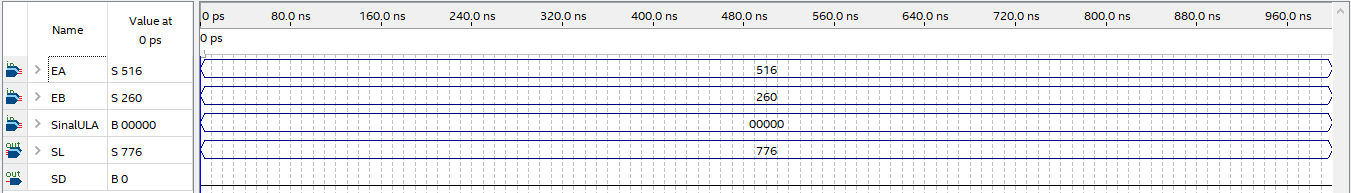
\includegraphics[width=1\textwidth]{Imagens/Onda_ULA_add.png} \\
  Fonte: o Autor.
  \label{fig:onda_ULA_add}
\end{figure}

Na \autoref{fig:onda_ULA_add}, a entrada EA recebe o valor 516 e a entrada EB o valor 260. O SinalULA contém o valor 000000, correspondente à operação de soma de EA com EB. O valor do resultado, conforme a \autoref{tab:op_ula}, é enviado para a saída padrão, SL. Nesse caso, como SD não é usada, deve permanecer com o valor zero.

Observe que o valor de SL é dado por 776, exatamente o valor de EA somado com EB (516 + 260), enquanto o valor de SD contém o valor zero. Portanto, esse comando para ULA funcionou corretamente.

\begin{figure}[H]
  \centering
  \caption{Instrução beq na ULA}
  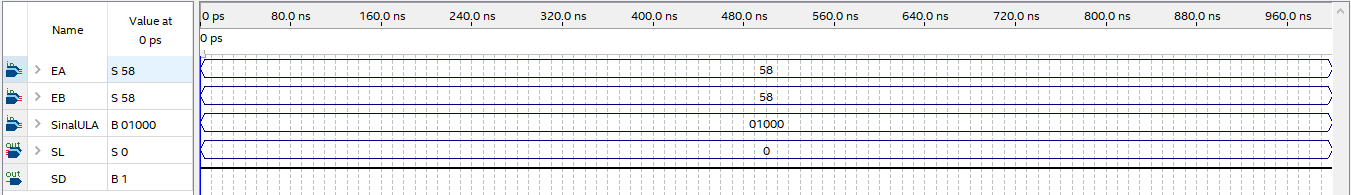
\includegraphics[width=1\textwidth]{Imagens/Onda_ULA_beq.png} \\
  Fonte: o Autor.
  \label{fig:onda_ULA_beq}
\end{figure}

Na \autoref{fig:onda_ULA_beq}, ambas entradas recebem o valor 58, enquanto SinalULA contém o valor 01000, correspondente, conforme a \autoref{tab:op_ula}, a instrução de beq. Desse modo, como as entradas são iguais, espera-se que o valor da saída SD seja 1. Além disso, por ser uma instrução de desvio, é esperado que a saída padrão tenha o valor zero.

Note que o valor das saídas é exatamente o valor esperado, com  SL tendo o valor zero, enquanto SD tem o valor 1, indicando que haverá salto condicional, pois as entradas são iguais.

\begin{figure}[H]
  \centering
  \caption{Instrução mul na ULA}
  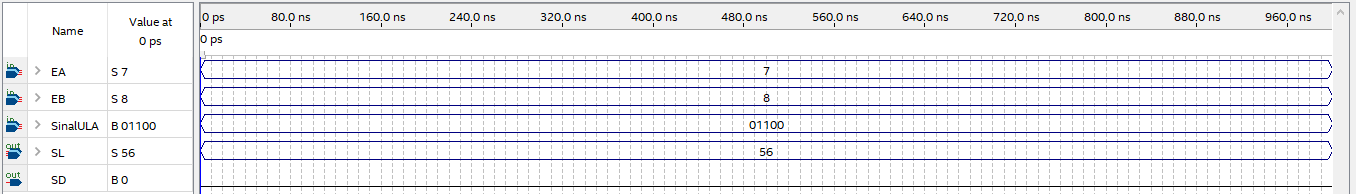
\includegraphics[width=1\textwidth]{Imagens/Onda_ULA_mul.png} \\
  Fonte: o Autor.
  \label{fig:onda_ULA_mul}
\end{figure}

A \autoref{fig:onda_ULA_mul} apresenta a entrada EA com valor 7, EB com o valor 8 e SinalULA com o valor 01100, correspondente à operação de multiplicação de EA por EB. 

Observe que o valor de SL é dado por 56, enquanto o valor de SD é dado por 0. Portanto, está funcionando corretamente, pois 7 multiplicado por 8 é 56. Além disso, como não é uma operação de salto, SD deve permanecer como zero.

\begin{figure}[H]
  \centering
  \caption{Instrução mul na ULA}
  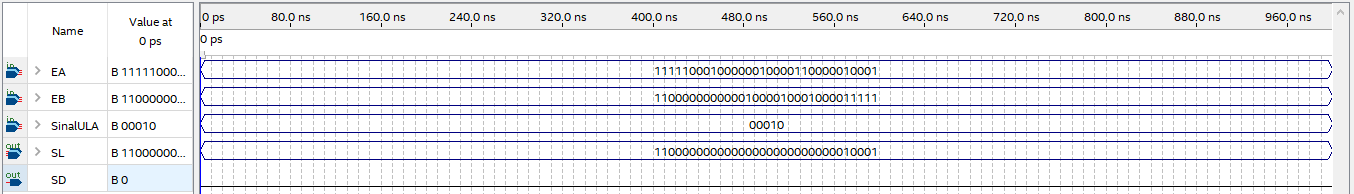
\includegraphics[width=1\textwidth]{Imagens/Onda_ULA_and.png} \\
  Fonte: o Autor.
  \label{fig:onda_ULA_and}
\end{figure}

Na \autoref{fig:onda_ULA_and}, é mostrado o comportamento da ULA para instrução and. Primeiramente, note que o valor de SD permanece em zero, o que é coerente por não ser uma instrução de salto condicional.

Os bits de SL assumem o valor 1 somente quando tanto a entrada EA quanto a entrada EB assumem o valor 1. Isso ocorre para o primeiro, quinto e dois últimos bits. Em todos os demais, o valor 1 está presente somente em EA ou somente em EB, de modo que o valor dos demais bits da saída é zero. Desse modo, a instrução está funcionando corretamente.

\section{Forma de onda do banco de registradores}

Para testar o banco de registradores, são usadas as entradas e saídas apresentadas na \autoref{tab:IO-banco_registradores}. A \autoref{fig:onda_banco_registradores} apresenta o comportamento do banco de registradores para um teste desenvolvido. A simulação foi feita toda de uma vez para garantir que não há dados sendo perdidos durante algum dos processos.

\begin{figure}[H]
  \centering
  \caption{Funcionamento do banco de registradores}
  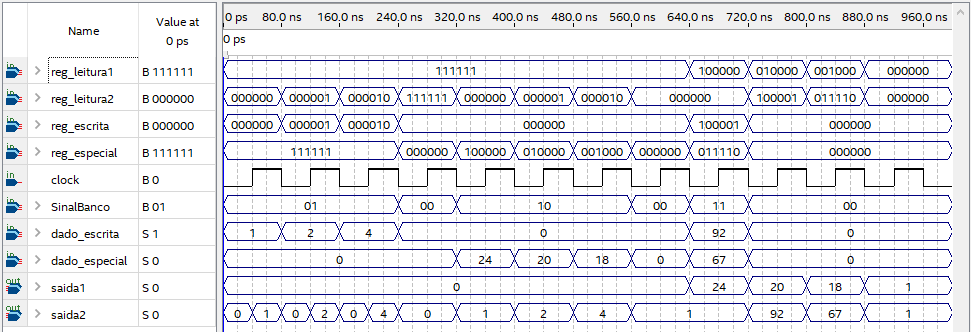
\includegraphics[width=1\textwidth]{Imagens/Onda_Banco_Registradores.png} \\
  Fonte: o Autor.
  \label{fig:onda_banco_registradores}
\end{figure}

Na \autoref{fig:onda_banco_registradores}, o primeiro registrador de leitura (reg\_leitura1) é o 111111. Como ele não tem um valor atribuído, o valor da saída1 permanece em zero enquanto ele é lido.

Nos três primeiros ciclos de clock, é usado o registrador de escrita (reg\_escrita), junto com o SinalBanco 01 (escrita no registrador de escrita) para escrever o valor 1 no registrador 000000, o valor 2 no registrador 000001 e o valor 4 no registrador 000010. 

Simultaneamente, o segundo registrador de leitura acompanha o valor desses registradores. Note que o valor da saída 2 só passa a ter o valor atribuído a partir da borda de subida do clock, conforme era esperado.

No quarto ciclo de clock, o SinalBanco é 00, logo não ocorrerá nenhuma escrita nem em reg\_escrita e nem em reg\_especial. Além disso, ambas as leituras são feitas do registrador 111111, que não possui valor atribuído, logo ambas as saídas são zero.

No quinto, sexto e sétimo ciclo de clock, o SinalBanco é 10 (escrita no registrador especial) e é utilizado o registrador especial para escrever os valores 24, 20 e 28, respectivamente, nos registradores 100000, 010000 e 001000. Enquanto isso, o registrador de escrita é o 000000, porém, devido ao SinalBanco, ele não tem seu valor atualizado.

Ao mesmo tempo em que essa escrita ocorre, é utilizado o segundo registrador de leitura para visitar os registradores que foram escritos nos primeiros três ciclos: 000000, 000001 e 000010 e os valores mostrados na saida2 continuam sendo os mesmos que foram escritos anteriormente: 1, 2 e 4, respectivamente.

No oitavo ciclo de clock o SinalBanco é 00, portanto não há escrita. O primeiro registrador de leitura continua sendo 111111, com o valor 0 na saida1 e o segundo registrador de leitura é o 000000, com o valor 1, que foi passado no início dessa simulação.

No nono ciclo é utilizado o SinalBanco 11 indicando que haverá escrita tanto em reg\_escrita quanto em reg\_especial. O registrador de escrita é o 100001 e o valor escrito (dado\_escrita) é 92. Enquanto o registrador especial é o 011110 e o valor de escrita (dado\_especial) é 67.

Além disso, no nono, décimo e décimo primeiro ciclos, é utilizado o primeiro registrador de leitura para verificar o valor dos registradores 100000, 010000 e 001000, escritos anteriormente. O valor da saída 1 apresenta os valores 24, 20 e 18, exatamente os valores passados para esses registradores.

Ademais, ainda nos décimo e décimo primeiro ciclos, é utilizado o segundo registrador de leitura para verificar os valores dos registradores 100001 e 011110, que foram escritos simultaneamente e os valores deles são, respectivamente, 92 e 67, o que é coerente com a escrita feita.

Por fim, no último ciclo nada ocorre, apenas é lido o registrador 000000 por ambos registradores de leitura e ambas saídas são 1, o que indica que, após ele receber o valor 1 no primeiro ciclo do clock, ele permaneceu com o seu valor inalterado durante todo o processo, sem ter seu dado perdido.

Sendo assim, pode-se concluir que o banco de registradores está funcionando corretamente.

\section{Forma de onda do módulo de processamento}

As entradas e saídas usadas estão descritas na \autoref{secao_integracao_ULA_banco}. A \autoref{fig:onda_integracao_ULA_banco} apresenta a forma de onda obtida ao testar esse módulo.

\begin{figure}[H]
  \centering
  \caption{Funcionamento da integração da ULA com o banco de registradores}
  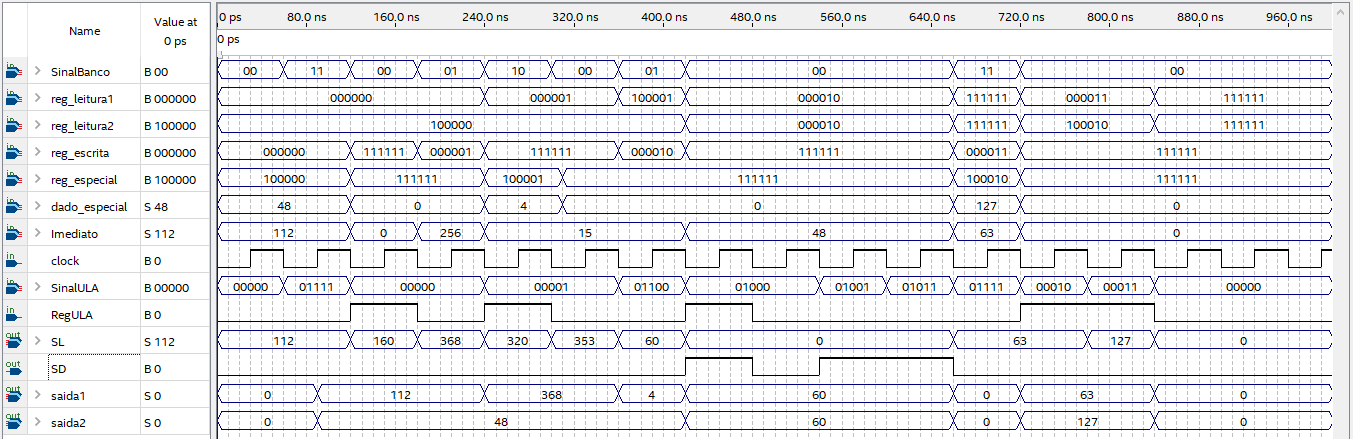
\includegraphics[width=1\textwidth]{Imagens/Onda_Integracao_ULA_Banco_mul.png} \\
  Fonte: o Autor.
  \label{fig:onda_integracao_ULA_banco}
\end{figure}

Primeiramente, observe que na \autoref{fig:onda_integracao_ULA_banco} as escritas, sinalizadas por sinalBanco, ocorrem somente nas bordas de subida do clock.

Durante o primeiro ciclo de clock, como RegULA é zero e o SinalULA é 000000, então é somado o valor presente no registrador 000000 com o imediato 112. Como o valor inicial de todo registrador é zero, o valor da saída padrão da ULA é dado por 0 somado com 112, o que resulta no 112 presente na saída SL.

No segundo ciclo, é usado o SinalBanco 11 para escrever no registrador de escrita 000000 e no registrador especial 100000. Os valores escritos em cada um são, respectivamente, o valor de SL e o valor do dado especial. 

Além disso, é utilizado o SinalULA 01111, o que corresponde ao comando de enviar como saída o valor da entrada EB. Nesse caso, como RegULA é 0, então o valor de EB é dado pelo imediato, que, nesse momento, vale 112. Portanto, o valor de SL permanece em 112. Sendo assim, é escrito o valor 112 em 000000 e o valor 48 em 100000.

Ainda durante o segundo ciclo, ambos os registradores que estão sendo escritos também estão sendo lidos. Por meio do valor de saida1 e saida2 é possível observar que o valor deles só foi atualizado na borda de subida do clock, conforme era esperado.

No terceiro ciclo é utilizado o SinalULA de soma junto com o sinal alto de RegULA para indicar que na segunda entrada da ULA será usado a segunda saída do banco de registradores. Sendo assim, é somado o valor das saídas do banco, respectivamente 112 e 48. Esse valor é passado para SL, que fica com o valor 160 como esperado.

No quarto ciclo, muda o sinal de RegULA, de modo que a ULA passa a usar a primeira saída do banco com um imediato, especificado como 256. Como o SinalULA se mantém, a saída é dada por 112 somado com 256, o que resulta em 368.

Além do mais, como o valor de SinalBanco é 01, é utilizado o valor da ULA para escrever no registrador de escrita passado, 000001, que recebe o valor de SL, 368.

No quinto ciclo, é mudado o primeiro registrador de leitura para observar o valor de 000001, escrito no ciclo anterior e seu valor de fato é 368. Ademais, é utilizado o sinal alto de RegULA para utilizar dois registradores na ULA e o SinalULA 00001 para indicar uma subtração.

Portanto é calculado o do valor de 000001, dado por 368, menos o valor do registrador 100000, dado por 48. O resultado é expresso por SL como 320, o que está correto.

Além disso, ainda durante o quinto ciclo, é utilizado o SinalBanco como 10 para realizar uma escrita especial. O registrador especial usado foi o 100001 e o dado especial passado foi 4.

No sexto ciclo muda o valor de RegULA, indicando o uso de registrador e imediato pela ULA. A operação feita continua sendo a subtração, pois o SinalULA não mudou. Sendo assim, é calculado 368, o valor do registrador 000001, menos 15, dado pelo imediato. O valor obtido é passado para SL como 353, conforme o esperado.

No sétimo ciclo o primeiro registrador de leitura é o 100001, que anteriormente recebeu o valor 4. Nesse ciclo é utilizado o SinalULA 01100 para realizar uma multiplicação. O sinal RegULA continua indicando registrador e imediato. Como o imediato é dado por 15, é calculado 4 vezes 15 e o resultado é 60.

Ademais, é utilizado o SinalBanco 01, o que indica que haverá apenas a escrita no registrador de escrita, que nesse caso é 000010. Portanto, é escrito o valor de SL, 60, no registrador de escrita.

No oitavo, nono, décimo e décimo primeiro ciclo, ambas as leituras são feitas do registrador 000010, que recebeu o valor 60 no ciclo anterior. Além disso, o valor do imediato permanece como 48.

No oitavo e nono ciclo, é utilizado o SinalULA 01000, indicando operação de beq. No oitavo ciclo, é utilizado RegULA como alto, portanto a comparação é feita entre os dois registradores lidos. Nesse caso, como é o mesmo registrador que é lido duas vezes, eles são iguais e, portanto, contêm o mesmo valor. Logo, o valor da saída SD é alto.

No nono, décimo e décimo primeiro ciclo, o valor de RegULA é baixo, portanto a ULA usa um registrador e um imediato. 

No nono ciclo, é usado o SinalULA 01000, ou seja, continua como beq, porém agora utilizando o valor do primeiro registrador lido e do imediato. Como o valor do primeiro registrador lido, 60, é diferente do valor do imediato, 48, o valor de SD é zero.

No décimo ciclo, o SinalULA é 01001, o que indica bne. Como 60 é diferente de 48, o valor de SD é um.

No décimo primeiro ciclo, o SinalULA é 01011, o que indica bgt. Como 60 é maior que 48, o valor de SD continua como um.

No décimo segundo ciclo, é lido duas vezes o registrador 111111, que não possui valor, portanto saida1 e saida2 têm o valor zero. Além disso, é usado SinalBanco 11 para escrever no registrador de escrita e no especial, dados respectivamente por 000011 e 100010.

O valor do dado especial é dado por 112, enquanto é usado como imediato o valor 63. Na ULA, é usado o SinalULA 01111, o que envia à saída diretamente o valor de EB, que nesse caso é o imediato, pois RegULA é 0. Sendo assim, SL, usado para escrever no registrador de escrita, é dado por 63.

Nos próximos dois ciclos são lidos os registradores 000011 e 100010, respectivamente. Além disso, RegULA indica que deve ser utilizado o valor de dois registradores na ULA.

No décimo terceiro ciclo o SinalULA é 00010, o que indica uma operação de and bit a bit. O valor 63 tem os bits menos significativos como 111111 e os demais como 0, enquanto o valor 127 tem os bits menos significativos como 1111111 e os demais são zero.

Portanto, uma operação de and vai resultar em 1 para os primeiros 6 bits e zero para os demais, o que corresponde ao próprio valor 63 e que é o valor da saída.

No décimo quarto ciclo só é mudada a operação da ULA para or. Isso faz com que, ao invés dos últimos seis bits, agora, são os últimos 7 que possuem o valor 1. Isso ocorre pois o sétimo bit menos significativo de 127 tem o valor 1, logo, ao fazer a operação or, ele permanece como 1. Sendo assim, a saída é o próprio 127, o que é coerente.

Desse modo, após percorrer essas operações funcionando corretamente, é possível concluir que a integração está funcionando como o esperado.

\section{Forma de onda memória principal}

Para simular a memória principal, foram utilizadas as entradas e saídas descritas na \autoref{tab:IO_memoria_dados}. A \autoref{fig:onda_memoria_principal} apresenta a forma de onda obtida durante o teste.

\begin{figure}[H]
  \centering
  \caption{Funcionamento da memória principal}
  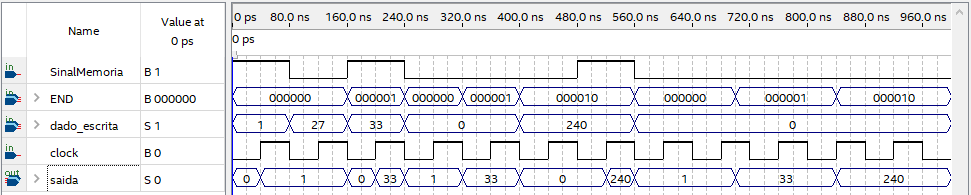
\includegraphics[width=1\textwidth]{Imagens/Onda_Memoria_Principal.png} \\
  Fonte: o Autor.
  \label{fig:onda_memoria_principal}
\end{figure}

Conforme explicado anteriormente, a memória constantemente realiza a operação de leitura e o SinalMemoria determina quando ocorrerá a operação de escrita no endereço END.

Note que neste teste há três momentos em que SinalMemória assume o valor 1. Nos três casos, note que o valor da saída só assumiu o valor de dado\_escrita após a borda de subida do clock, conforme o esperado.

Além disso, após as escritas, ao retornar para os mesmos registradores, o valor lido continua sendo o mesmo valor escrito, portanto não está ocorrendo nenhuma perda e não há nenhuma escrita indevida de valores.

Desse modo, o comportamento da memória principal está totalmente dentro do esperado e funciona corretamente.

\section{Forma de onda memória de instruções}

A princípio, a \autoref{fig:teste_memoria_instrucoes} apresenta o documento ``single\_port\_rom\_init.txr'', que contém as instruções a serem lidas. 

\begin{figure}[H]
  \centering
  \caption{Instruções utilizadas no teste da memória de instruções}
  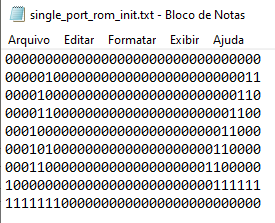
\includegraphics[width=0.5\textwidth]{Imagens/Teste_Memoria_Instrucoes.png} \\
  Fonte: o Autor.
  \label{fig:teste_memoria_instrucoes}
\end{figure}

Note que na \autoref{fig:teste_memoria_instrucoes} acima, há 9 linhas, que correspondem a 9 instruções. Cada linha possui 32 bits, portanto, os 6 primeiros são o Opcode e os outros 26 são os operandos. 

Nesse caso, por ser apenas um teste, os operandos foram tomados como valores baixos para facilitar a representação deles em decimal. Porém, em um caso real não faz sentido olhar para esses campos como um decimal, pois, na realidade, há vários operandos nesses 26 bits, conforme cada um dos formatos de instruções.

A partir dessa entrada, foi desenvolvida a \autoref{tab:Separacoes_do_teste_instrucoes} que apresenta esses mesmos valores com o campo de Opcode separado dos operandos. Nessa tabela há os valores em binário, conforme a \autoref{fig:teste_memoria_instrucoes} acima, além de outras duas colunas que apresentam o campo de Opcode e operandos em decimal.

\setlength{\tabcolsep}{10pt} % Define o tamanho das colunas
\begin{table}[ht]
\centering
\caption{Separação das instruções do teste da memória em Opcode e operandos}
\label{tab:Separacoes_do_teste_instrucoes}
\begin{tabular}{|>{\ttfamily}c|>{\ttfamily}c|c|c|}
\hline
\multicolumn{2}{|c|}{Binário} & \multicolumn{2}{|c|}{Decimal} \\
\hline
Opcode (6 bits) & Operandos (26 bits) & Opcode & Operandos \\
\hline
000000 & 00000000000000000000000000 & 0 & 0 \\
000001 & 00000000000000000000000011 & 1 & 3 \\
000010 & 00000000000000000000000110 & 2 & 6 \\
000011 & 00000000000000000000001100 & 3 & 12 \\
000100 & 00000000000000000000011000 & 4 & 24 \\
000101 & 00000000000000000000110000 & 5 & 48 \\
000110 & 00000000000000000001100000 & 6 & 96 \\
100000 & 00000000000000000000111111 & 32 & 63 \\
111111 & 10000000000000000000000000 & 63 & 33554432 \\
\hline
\end{tabular}
\vspace{-0.5em}
\begin{center}
Fonte: o Autor.
\end{center}
\end{table} 

Para simular a memória de instruções, foram utilizadas as entradas e saídas descritas na \autoref{tab:IO_memoria_instrucoes}. A \autoref{fig:onda_memoria_instrucoes} apresenta a forma de onda obtida durante o teste.

\begin{figure}[H]
  \centering
  \caption{Funcionamento da memória de instruções}
  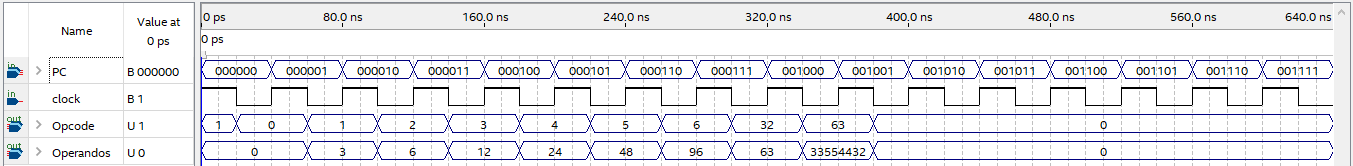
\includegraphics[width=1\textwidth]{Imagens/Onda_Memoria_Instrucoes.png} \\
  Fonte: o Autor.
  \label{fig:onda_memoria_instrucoes}
\end{figure}

Note que nessa simulação o sinal de clock, diferente das demais simulações, começa em nível alto. Isso foi feito apenas para facilitar a visualização da atualização da saída apenas nas bordas de descida do clock.

A princípio, tanto o valor de Opcode é 1, isso foi definido explicitamente para garantir que o processador não execute uma instrução indevida. Enquanto isso, o valor de Operandos é zero, pois foi definido assim. 

Na primeira borda de descida do clock, o valor de Opcode assume o valor da primeira instrução que é 000000, enquanto o valor de Operandos não muda, pois a primeira instrução, apresentada na \autoref{fig:teste_memoria_instrucoes}, é composta apenas de zeros, então o valor dele permanece em zero.

Em sequência, nos próximos ciclos de clock, os valores lidos no campo de Opcode são respectivamente 1, 2, 3, 4, 5, 6,32 e 63, exatamente os valores obtidos ao converter o campo de Opcode para decimal na \autoref{tab:Separacoes_do_teste_instrucoes}. Nesse mesmo período, o valor do campo Operando é dado por 3, 6, 12, 24, 48, 96, 63 e 33.554.432, o que também está coerente com a \autoref{tab:Separacoes_do_teste_instrucoes}.

Após a leitura desses valores, as saídas voltam a ser zero. Isso ocorre pois foram passadas nove instruções pelo arquivo ``single\_port\_rom\_init.txr'', conforme mostrado pela \autoref{fig:teste_memoria_instrucoes}. Portanto, há instruções somente entre os endereços 000000 e 001000.

Após ler todas as instruções, o valor lido passa a ser zero, pois não há nenhuma instrução. Isso foi utilizado para determinar o código da instrução HLT como 000000 na \autoref{opcode_lista_bin_zero}, pois, caso leia uma instrução inválida, o processador será interrompido.

Sendo assim, a memória de instruções está funcionando de acordo com o esperado.

\section{Forma de onda do PC}

Para testar o módulo do PC foram usadas as entradas e saídas presentes na \autoref{tab:IO_PC}. A \autoref{fig:onda_PC} mostra a forma de onda obtida durante o teste.

\begin{figure}[H]
  \centering
  \caption{Funcionamento do módulo do PC}
  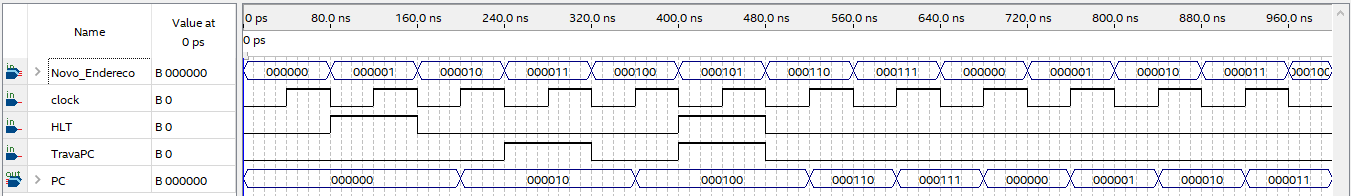
\includegraphics[width=1\textwidth]{Imagens/Onda_PC.png} \\
  Fonte: o Autor.
  \label{fig:onda_PC}
\end{figure}

Na \autoref{fig:onda_PC} a variável Novo\_Endereço foi incrementada gradualmente. Observe que o valor de PC foi atualizado, com base no valor de Novo\_Endereço, sempre durante a borda de subida do sinal de clock. Posteriormente, foi necessário mudar esse comportamento para a borda de descida do clock.

Porém, quando um dos sinais, HLT ou TravaPC, está com sinal alto, o valor do PC não é atualizado, como era esperado. Sendo assim, o módulo do PC está funcionando corretamente.

\section{Sobre a unidade de controle}

Para a unidade de controle não foram feitos testes com forma de onda, pois como ela funciona como um circuito combinacional, não há nenhum comportamento que valha a pena ser observado na forma de onda. 

Seria possível observar os valores dos sinais de controle, mas isso não contribui para a compreensão do módulo ou o correto funcionamento dele. Para isso, uma forma mais confiável de se testar é por meio da execução de instruções diretamente na versão final, acompanhando todas as etapas e se a instrução é realizada corretamente.

\section{Forma de onda do módulo de entrada e saída}

A \autoref{fig:onda_entrada_saida} apresenta a forma de onda obtida ao testar o módulo de entrada e saída com um debounce de 3 ciclos de clock no botão. Na forma de onda não é possível manter o debouncer original, de 60000 ciclos de clock, pois não seria possível percorrer tantos ciclos de clock em uma única simulação e dificultaria a compreensão.

\begin{figure}[H]
  \centering
  \caption{Funcionamento do módulo de entrada e saída}
  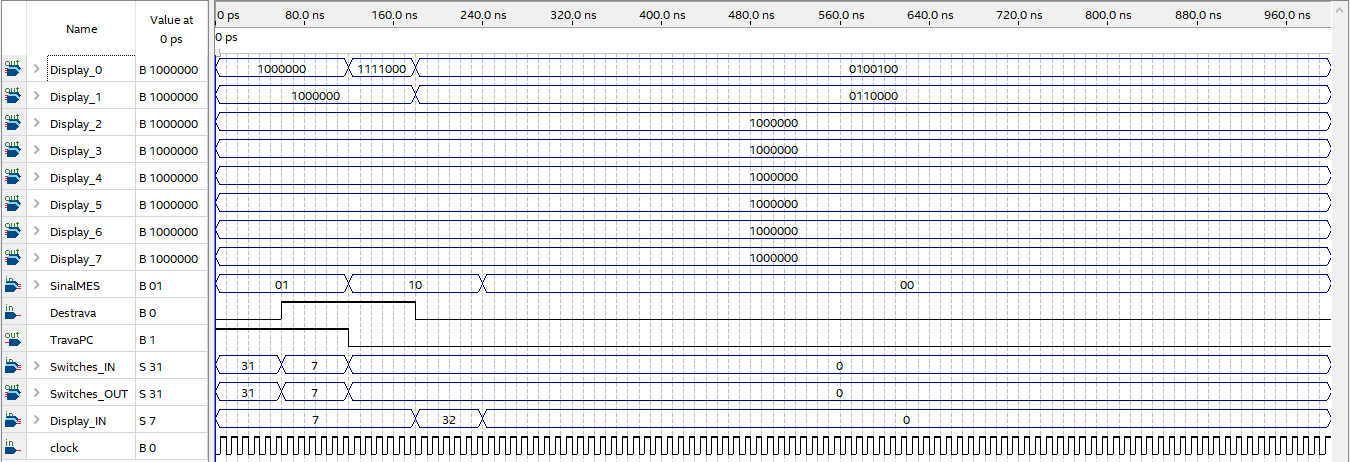
\includegraphics[width=1\textwidth]{Imagens/Onda_Modulo_Entrada_Saida.png} \\
  Fonte: o Autor.
  \label{fig:onda_entrada_saida}
\end{figure}

Note que na \autoref{fig:onda_entrada_saida} valor de Switches\_IN é estendido corretamente para Switches\_OUT. Além disso, assim que a instrução de IN começa, o valor de TravaPC se torna um e isso deve impedir o PC de avançar; nesse caso em particular, isso não ocorre porque está sendo testado o módulo isolado.

Ademais, ao pressionar o botão de destravar, somente após três ciclos de clock completos, ou seja, três subidas e descidas do clock, que o valor de TravaPC volta a ser zero.

Por fim, o valor escrito no display só muda a partir do momento que o SinalMES para a indicar um comando OUT (01), em um primeiro momento o display zero escreve o valor sete, acompanhando o valor de Display\_IN 7 e depois o valor dois para o Display\_IN 32, ou seja, corretamente acompanhou o valor da unidade. Enquanto o display um passa a escrever o valor três para o Display\_IN 32.

Após o SinalMES indicar o fim do comando OUT, os displays ficam com o último valor escrito neles, sem se alterar mais até que eventualmente ocorra um novo comando OUT. Dessa forma, o módulo de entrada e saída está funcionando corretamente.

\section{Integração final}

O teste final para comprovar o funcionamento de tudo se deu por meio da implementação da integração de todos os códigos desenvolvidos no kit FPGA. Para isso, foram elaborados dois códigos para testar o comportamento do processador.

Os códigos desenvolvidos estão presentes na \autoref{fig:codigo1} e \autoref{fig:codigo2} abaixo.

\begin{figure}[H]
  \centering
  \caption{Código 1 - Fibonacci}
  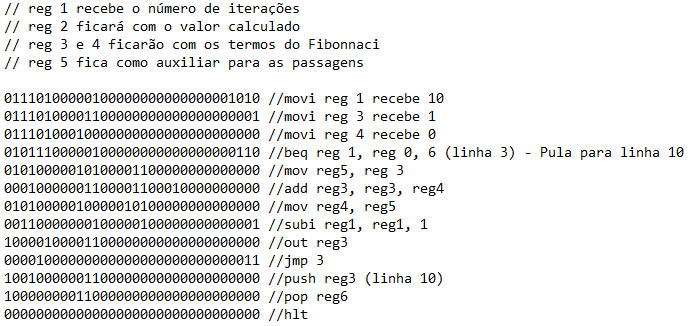
\includegraphics[width=1\textwidth]{Imagens/Codigo1.png} \\
  Fonte: o Autor.
  \label{fig:codigo1}
\end{figure}

\begin{figure}[H]
  \centering
  \caption{Código 2 - Calculo da média aritmética}
  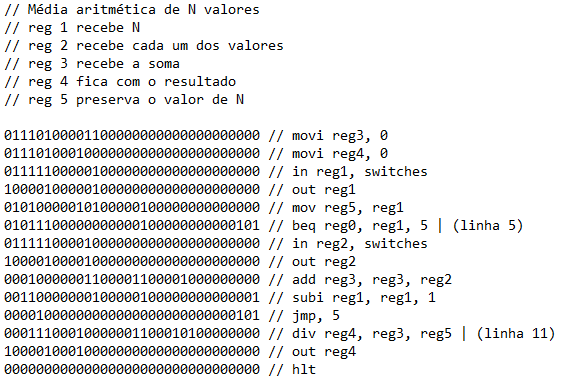
\includegraphics[width=1\textwidth]{Imagens/Codigo2.png} \\
  Fonte: o Autor.
  \label{fig:codigo2}
\end{figure}

O primeiro código implementa um algoritmo para calcular o valor do décimo termo da sequência de Fibonacci sem contar o termo 1 duas vezes.

O segundo código calcula a média de n valores. Para isso, ele recebe um valor n pelos switches e depois o valor de cada um dos n valores e, em seguida, calcula a média aritmética deles. Ademais, para cada valor lido ele também escreve no display para confirmar que foi lido corretamente.

É importante pontuar que para o código ser utilizado pelo processador foi preciso salvar no arquivo ``single\_port\_rom\_init.txt'' apenas os números em binário, sem os comentários.

A \autoref{fig:processador_fib} abaixo apresenta o resultado para o primeiro código e o valor escrito, 89, é coerente com o resultado esperado. Portanto, funcionou corretamente.

\begin{figure}[H]
  \centering
  \caption{Resultado - Código 1 - Fibonacci}
  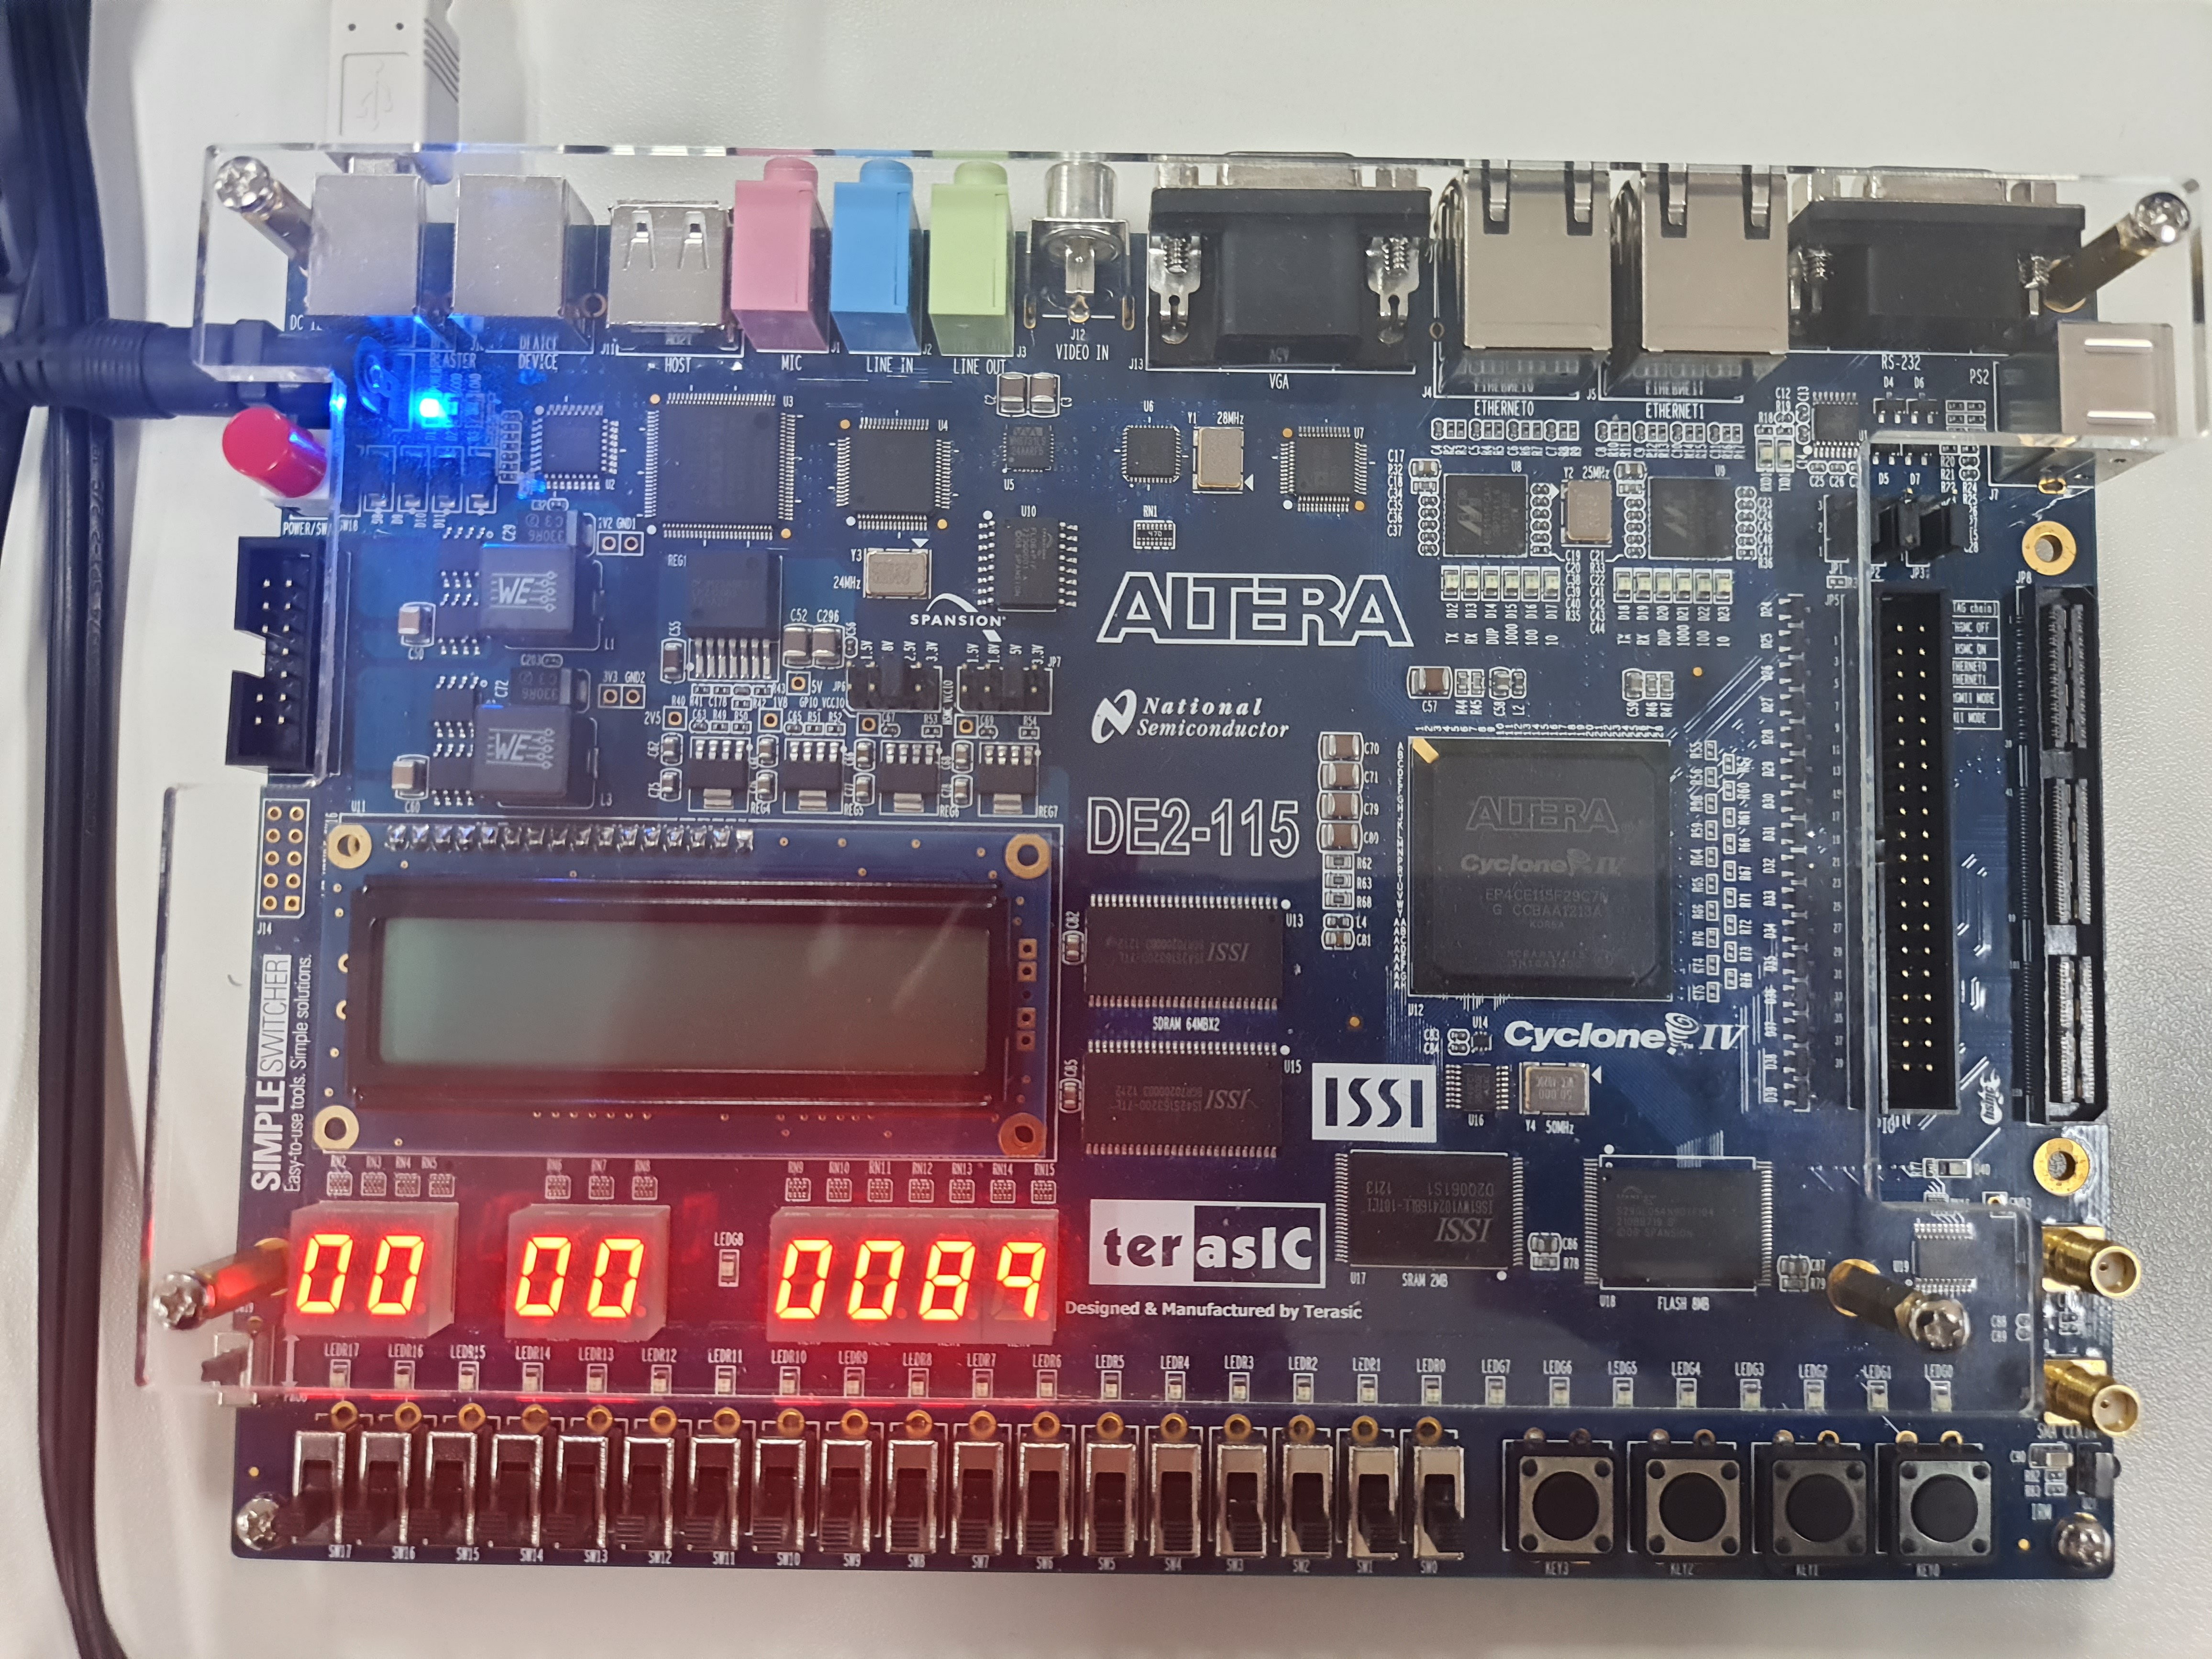
\includegraphics[width=0.7\textwidth]{Imagens/Processador_fib.jpg} \\
  Fonte: o Autor.
  \label{fig:processador_fib}
\end{figure}

As \autoref{fig:processador_0}, \autoref{fig:processador_1}, \autoref{fig:processador_2}, \autoref{fig:processador_3}, \autoref{fig:processador_4} e \autoref{fig:processador_5} apresentam a sequência de entradas utilizadas com o código 2, bem como o valor do resultado. Primeiramente, na primeira das figuras, o processador inicializou mostrando o valor zero no display. Em seguida, na segunda figura, foi inserido o primeiro valor como 4, que corresponde ao número de valores no cálculo da média. 

Após isso, na \autoref{fig:processador_2}, \autoref{fig:processador_3} e \autoref{fig:processador_4}, são inseridos nas entradas os valores 6, 4 e 7, respectivamente. Na figura \autoref{fig:processador_5} é inserido o valor 3, porém, imediatamente após inserir o último valor, a média é calculada e escrita no display.

Sendo assim, somando os valores 6 + 4 + 7 + 3 = 20, como foram somados 4 termos, a resposta deve ser 20/4 = 5, o que é exatamente o valor exibido ao final. Desse modo, pode-se concluir que o código funcionou corretamente, bem como o processador de um modo geral.

\begin{figure}[H]
  \centering
  \caption{Inicio - Código 2 - Calculo da média aritmética}
  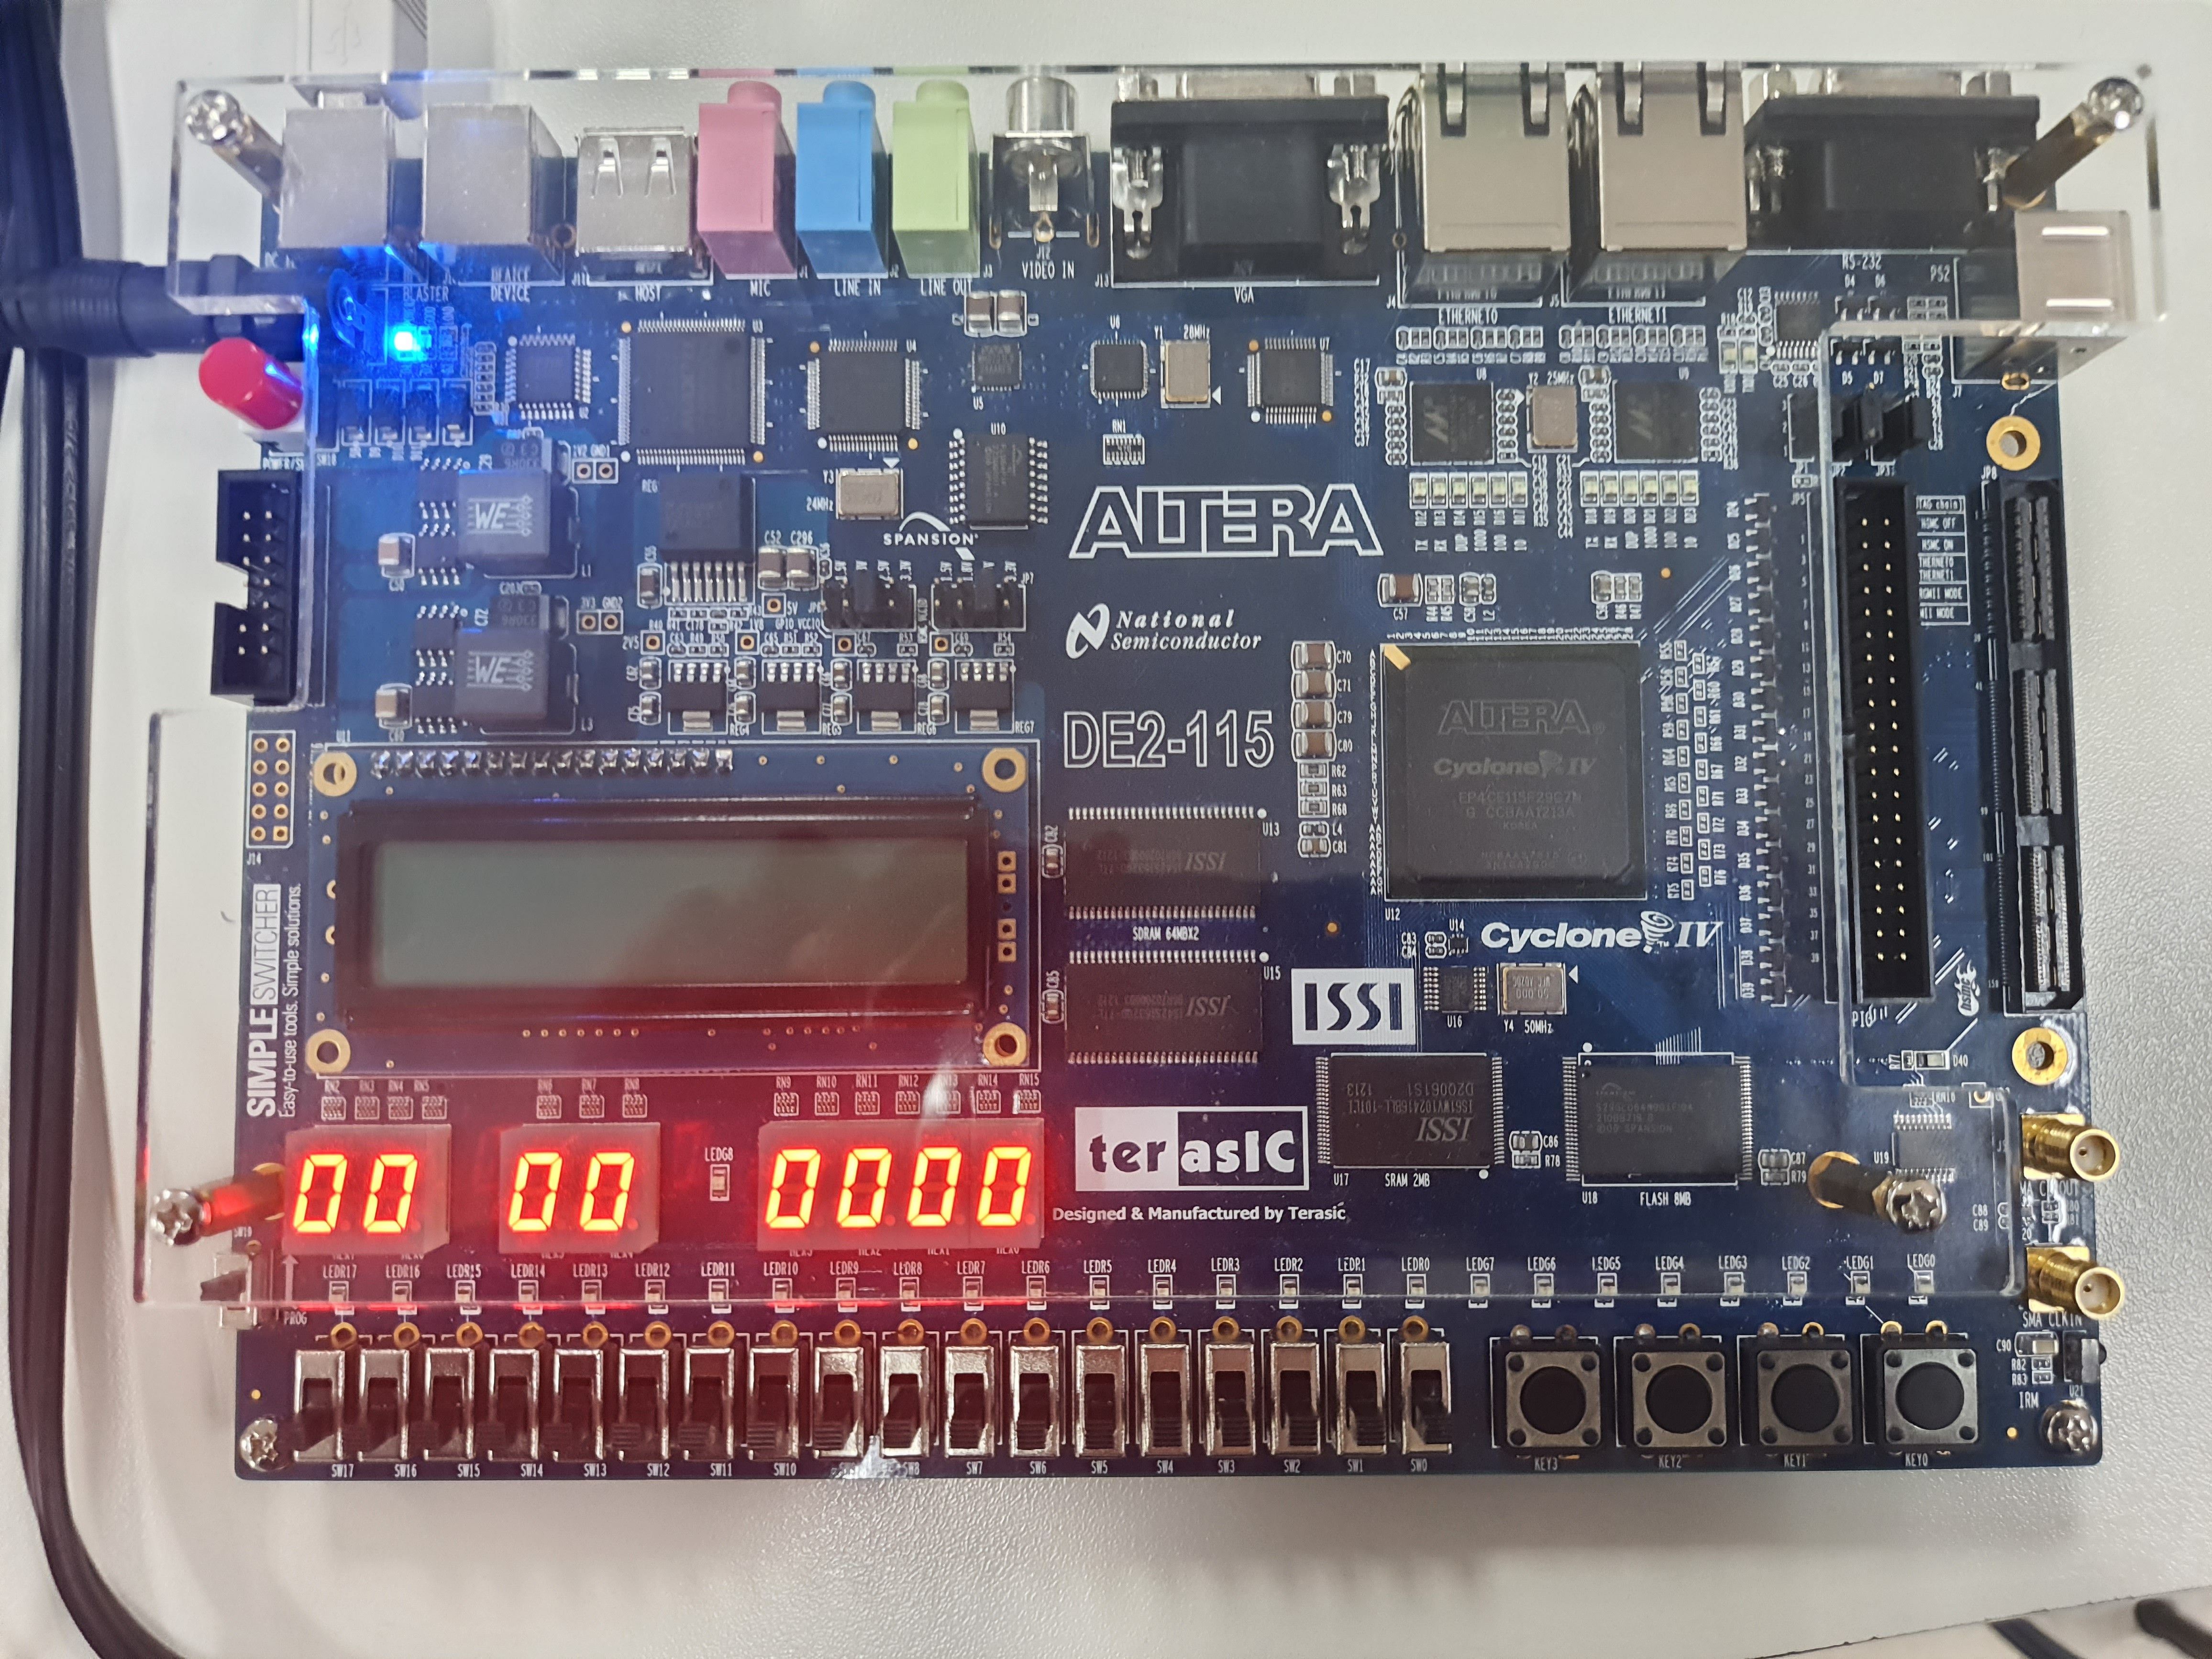
\includegraphics[width=0.7\textwidth]{Imagens/Processador_0.jpg} \\
  Fonte: o Autor.
  \label{fig:processador_0}
\end{figure}

\begin{figure}[H]
  \centering
  \caption{Valor de n - Código 2 - Calculo da média aritmética}
  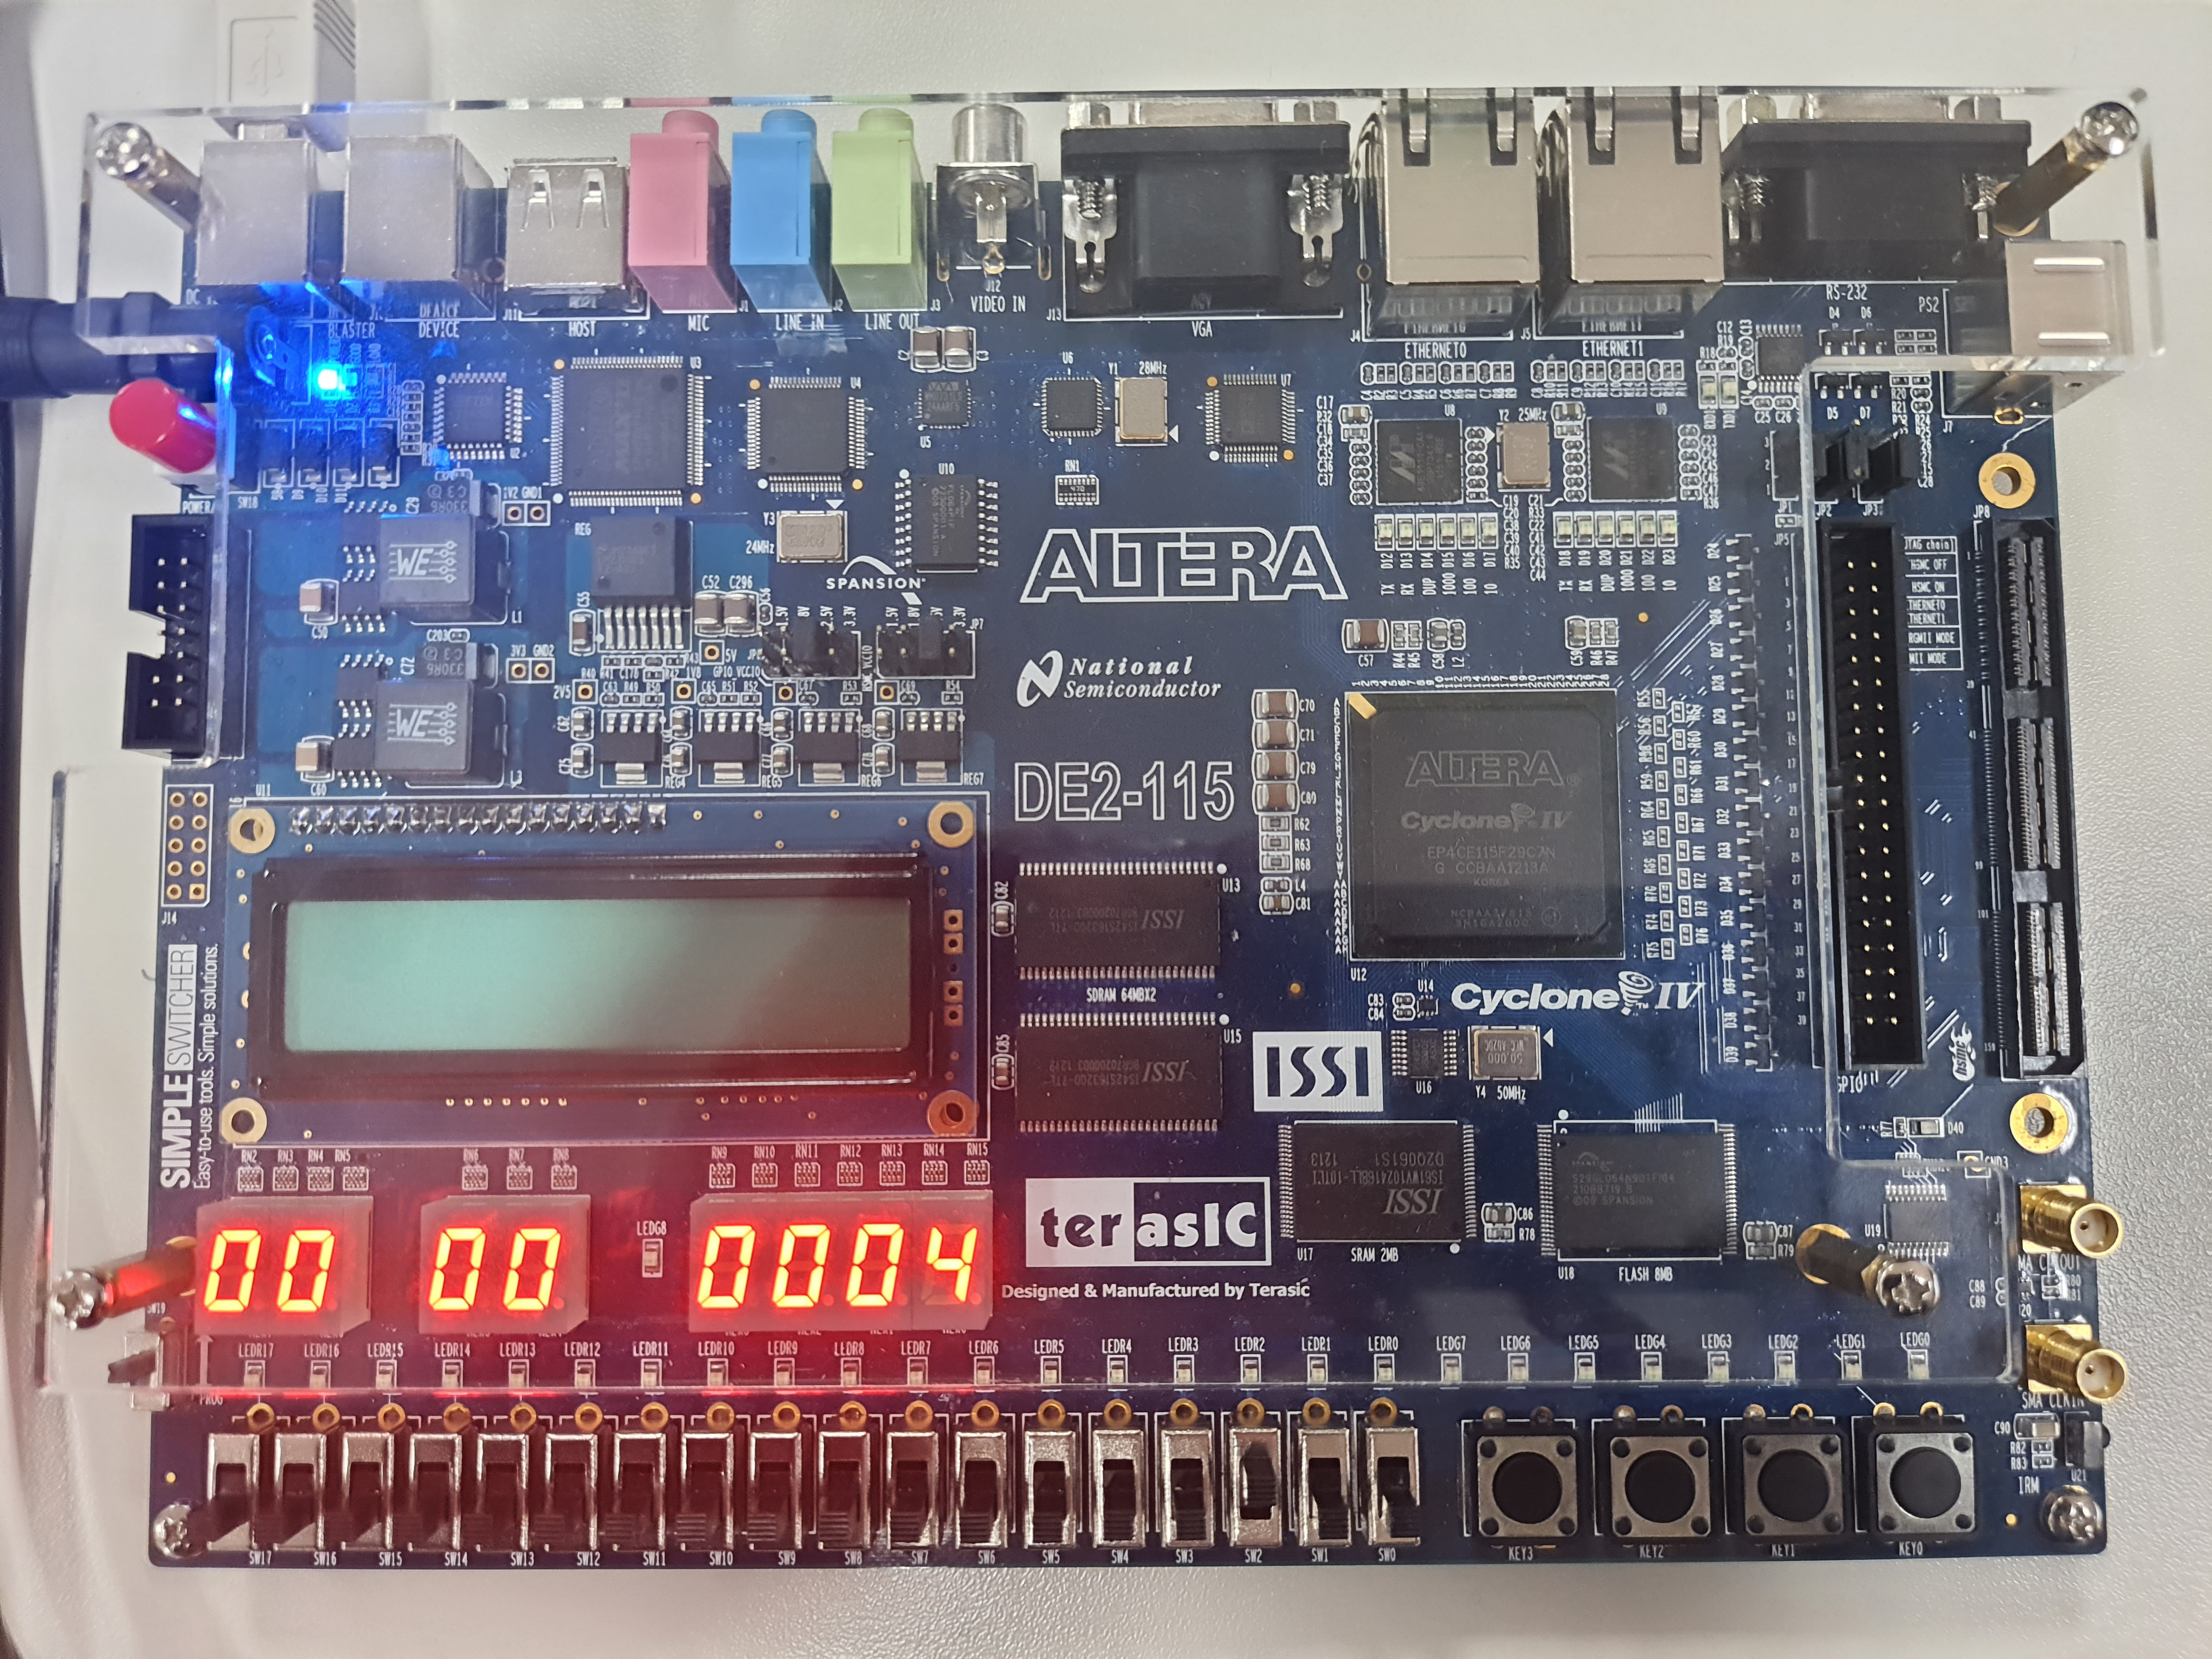
\includegraphics[width=0.7\textwidth]{Imagens/Processador_1.jpg} \\
  Fonte: o Autor.
  \label{fig:processador_1}
\end{figure}

\begin{figure}[H]
  \centering
  \caption{Número 1 - Código 2 - Calculo da média aritmética}
  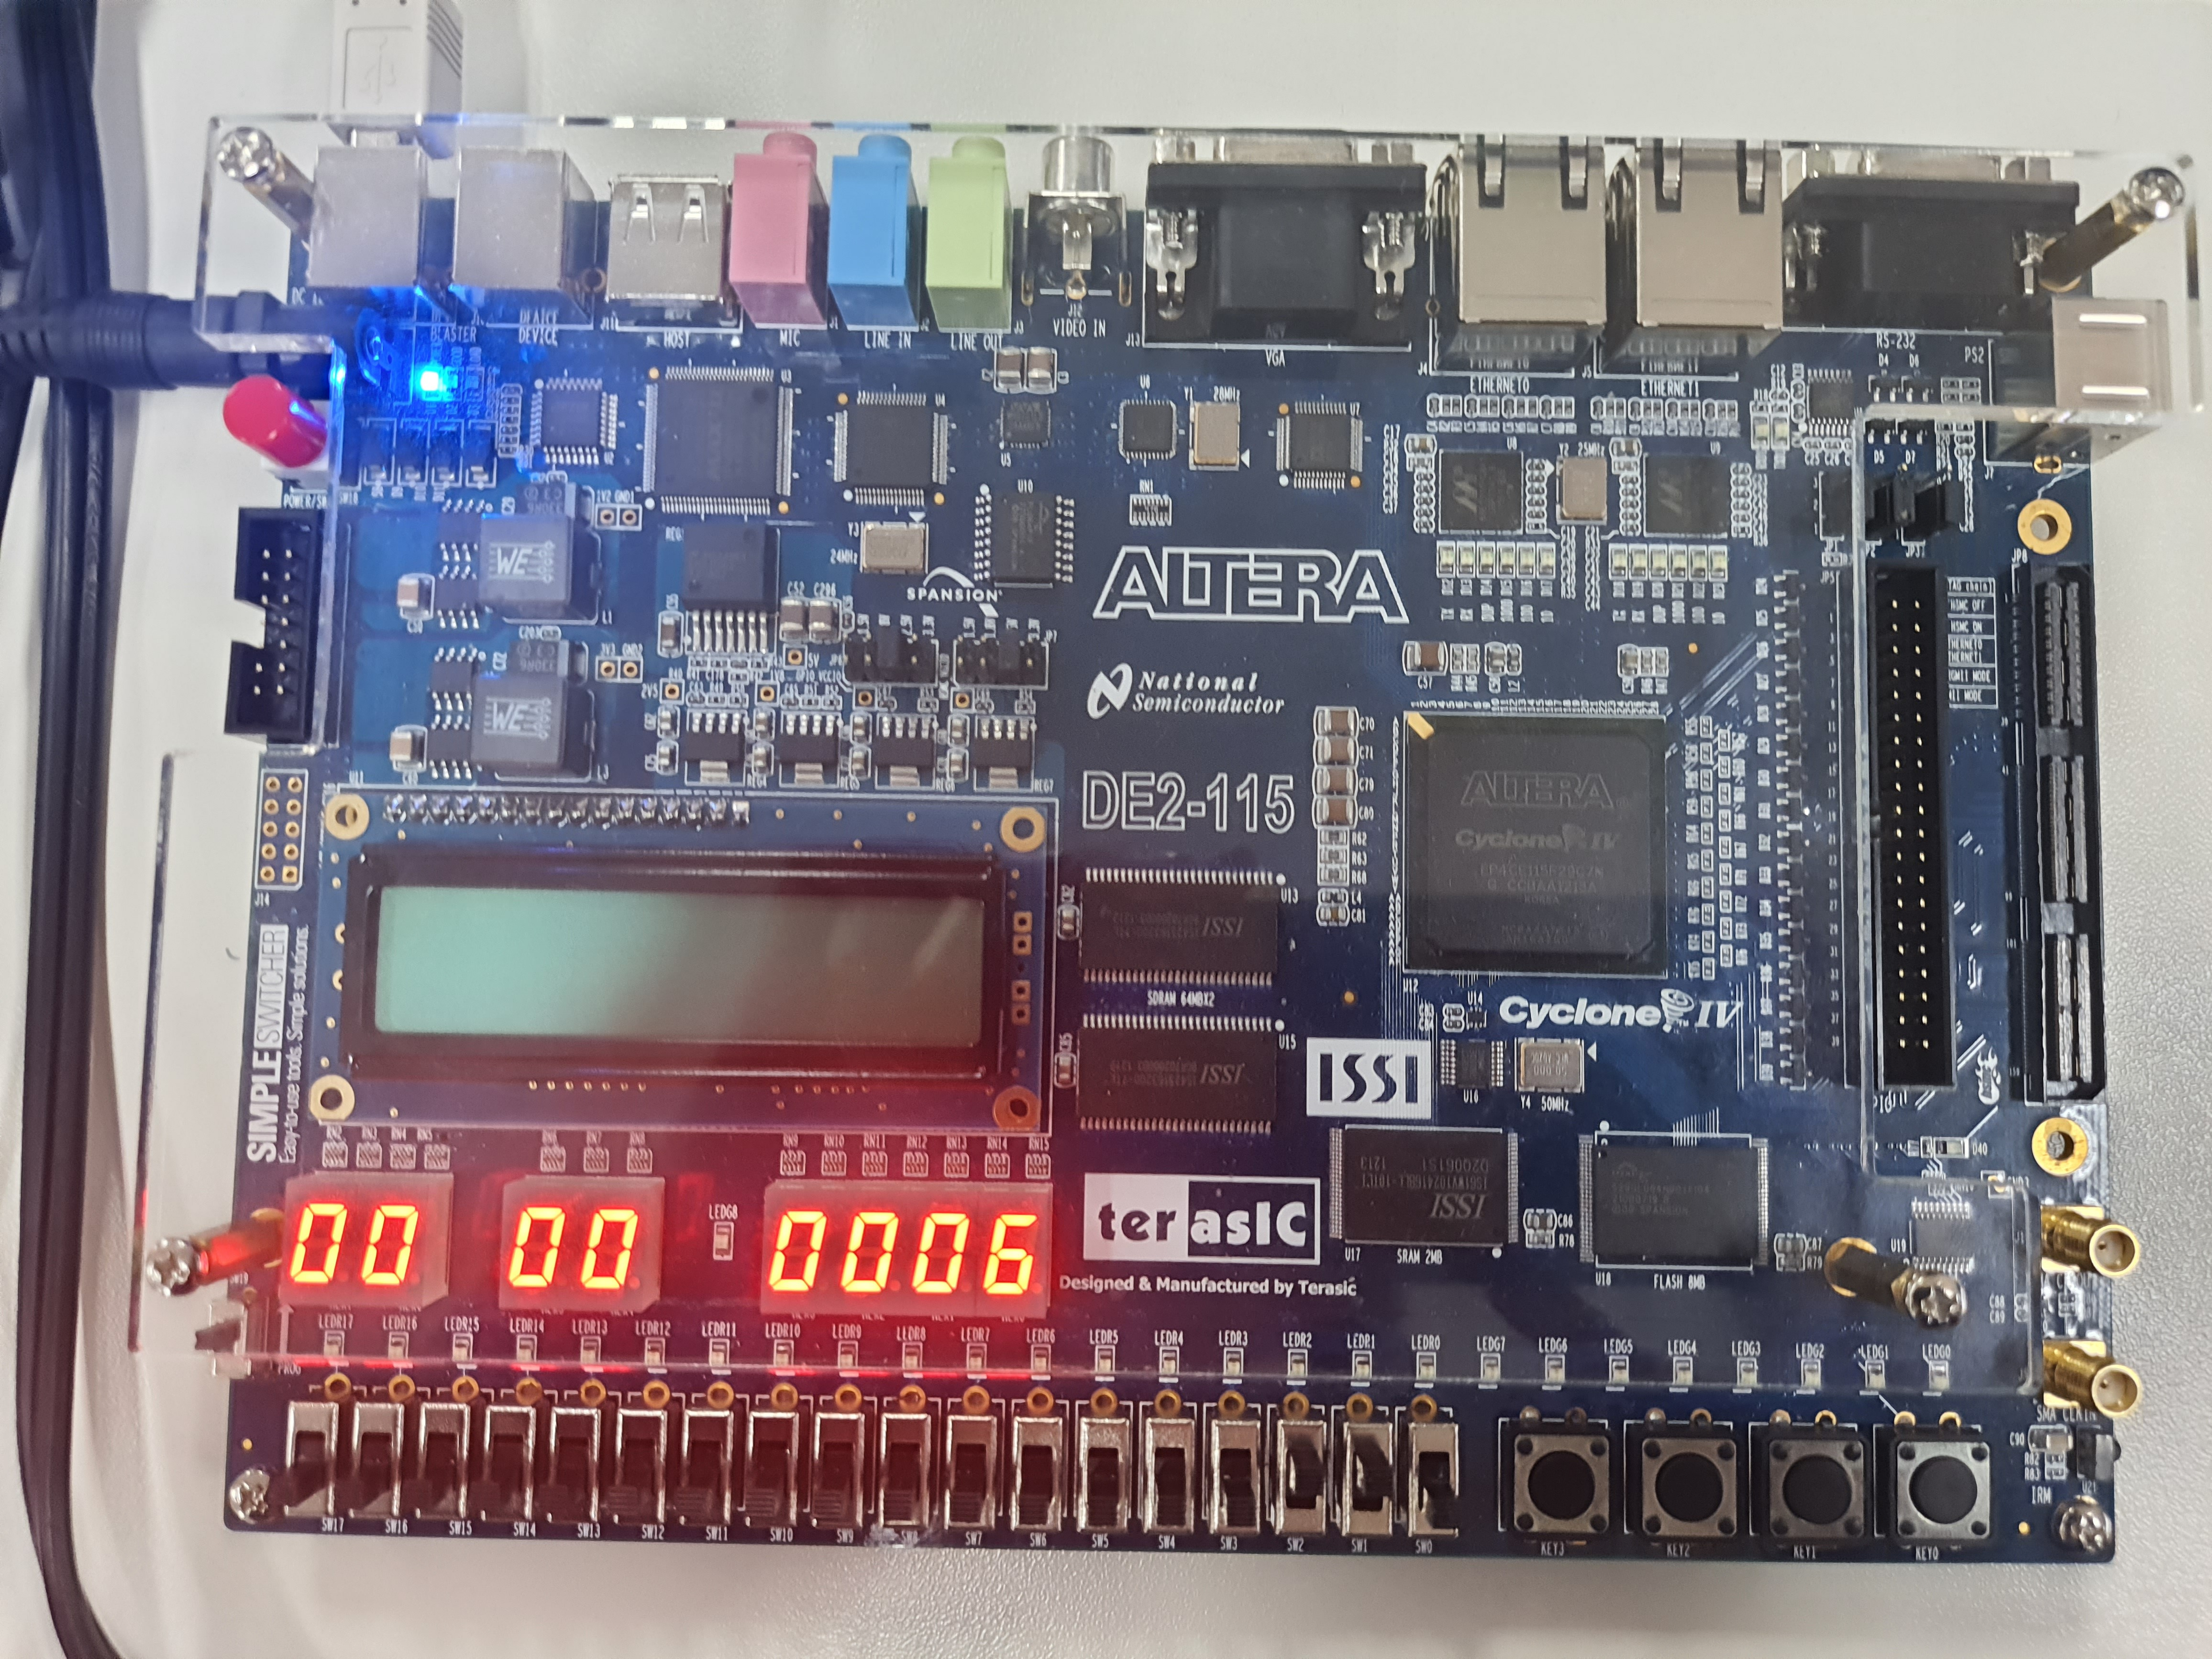
\includegraphics[width=0.7\textwidth]{Imagens/Processador_2.jpg} \\
  Fonte: o Autor.
  \label{fig:processador_2}
\end{figure}

\begin{figure}[H]
  \centering
  \caption{Número 2 - Código 2 - Calculo da média aritmética}
  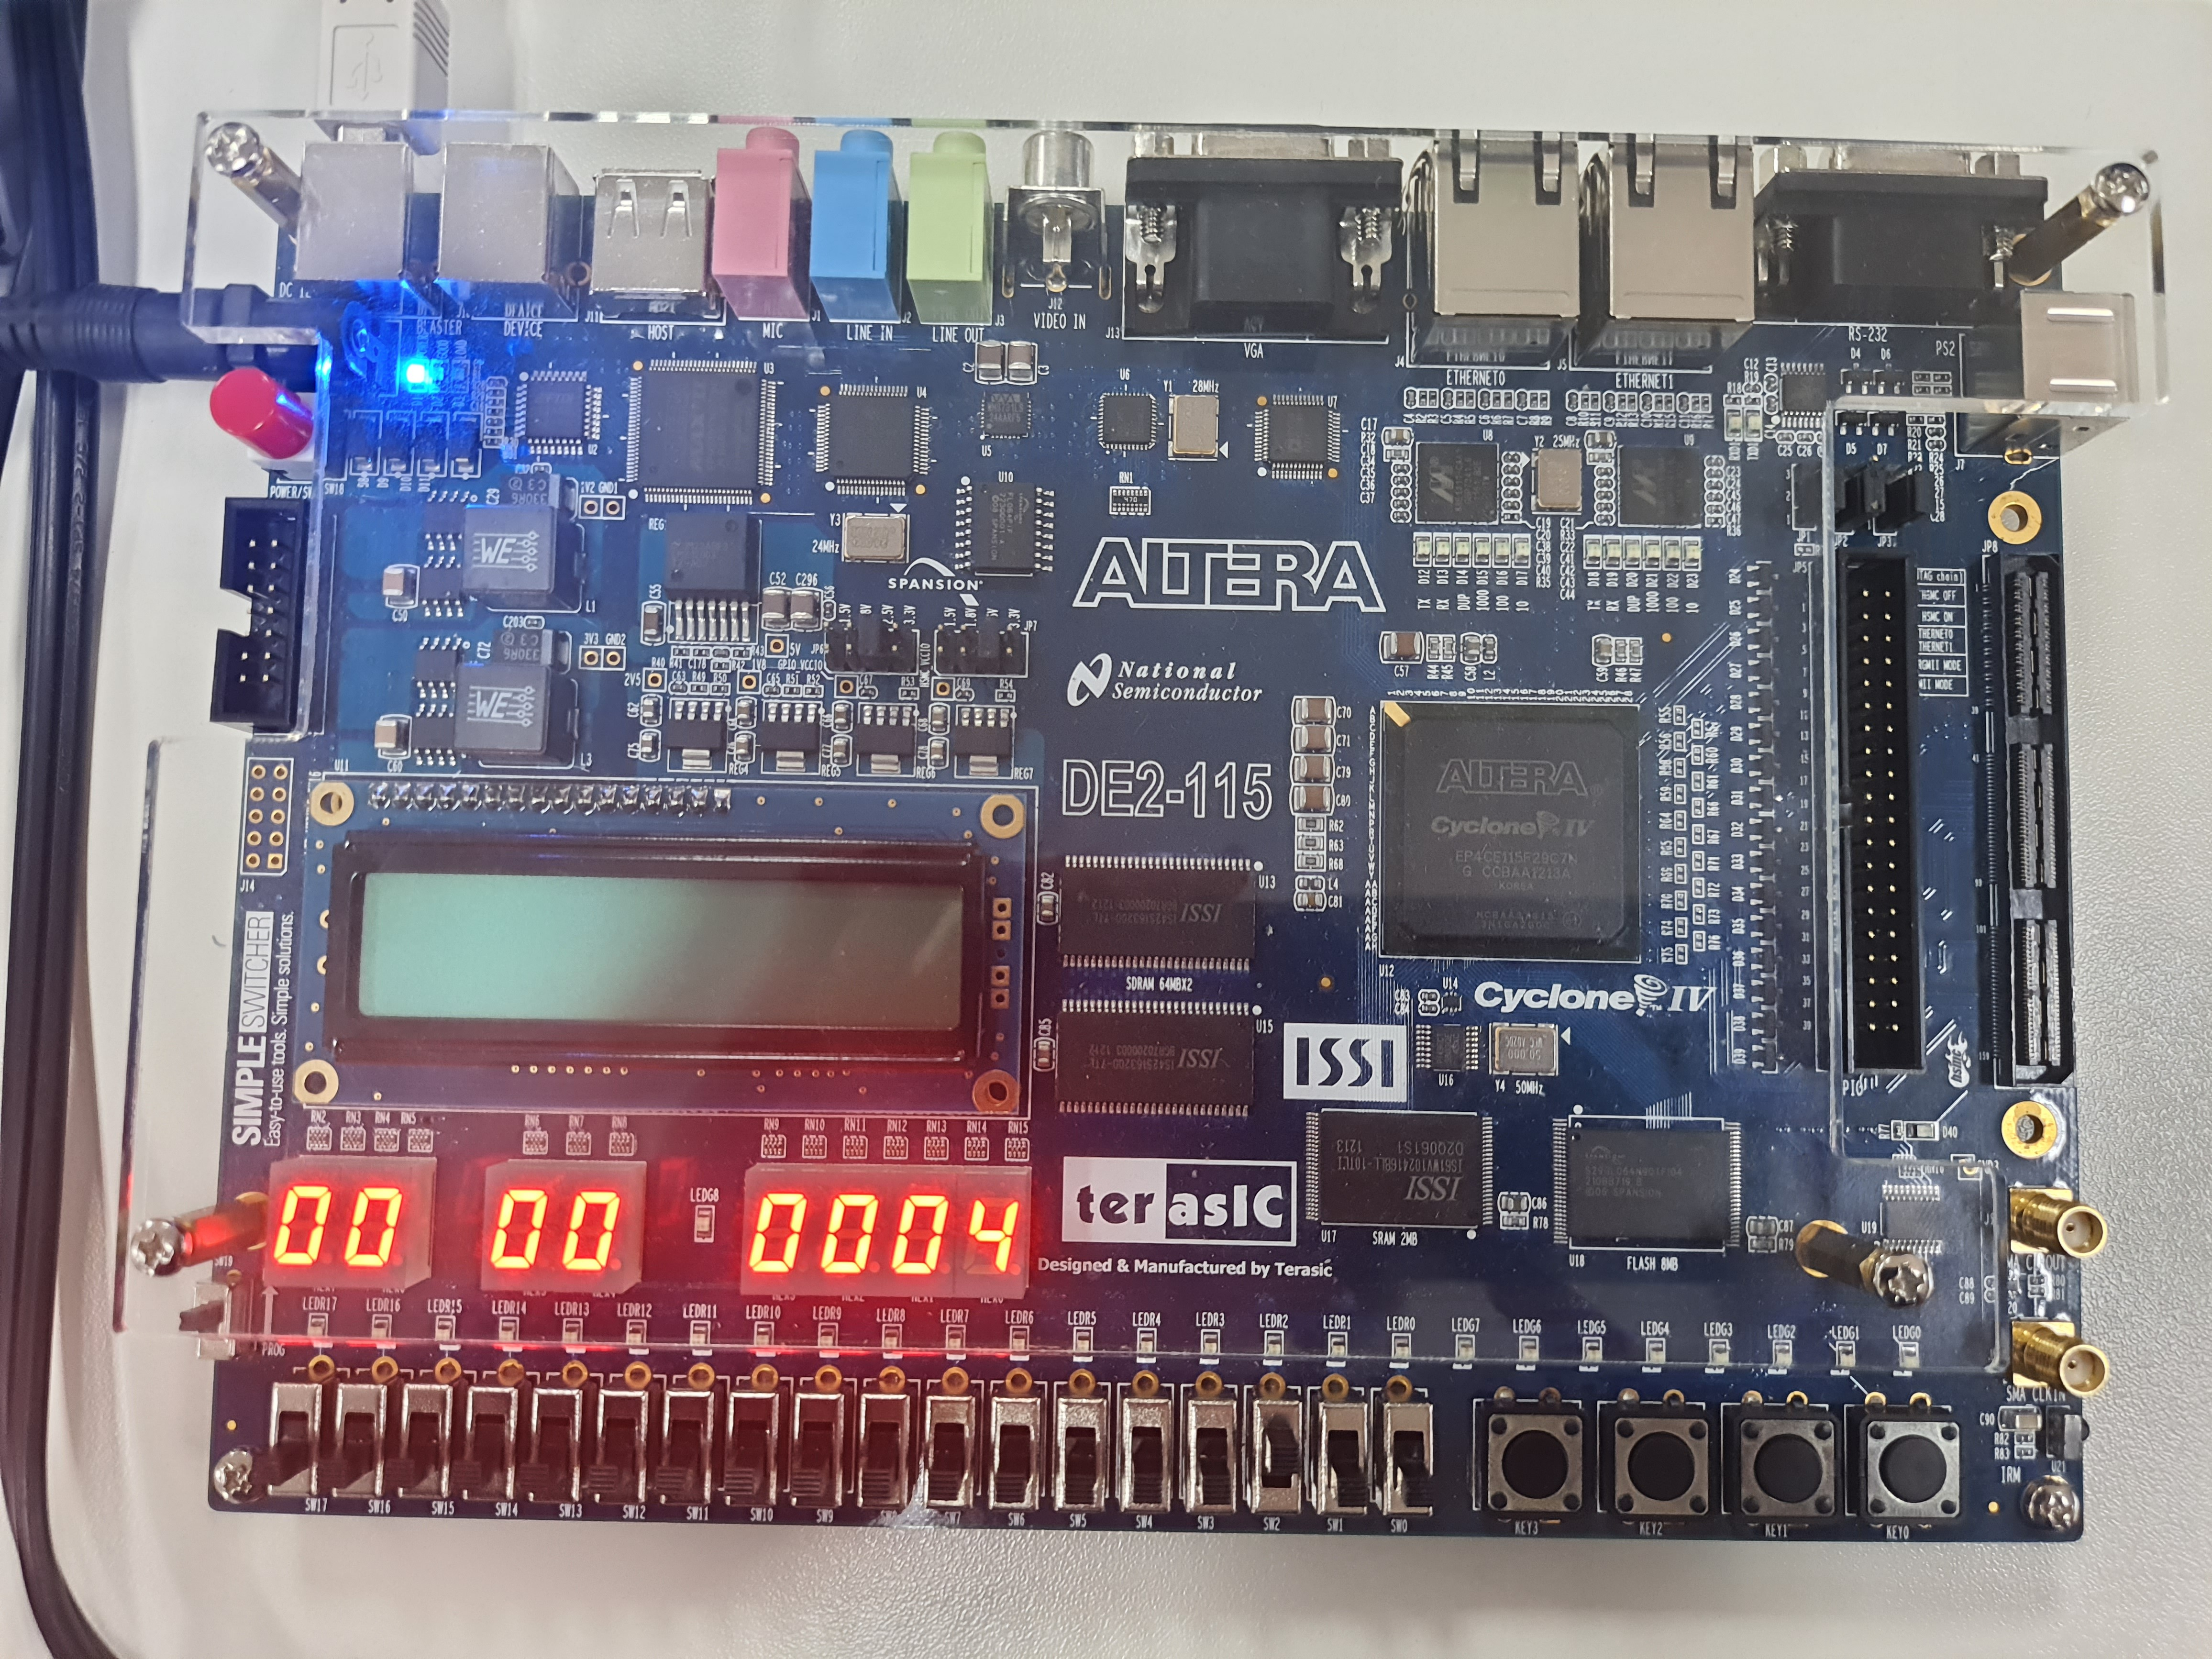
\includegraphics[width=0.7\textwidth]{Imagens/Processador_3.jpg} \\
  Fonte: o Autor.
  \label{fig:processador_3}
\end{figure}

\begin{figure}[H]
  \centering
  \caption{Número 3 - Código 2 - Calculo da média aritmética}
  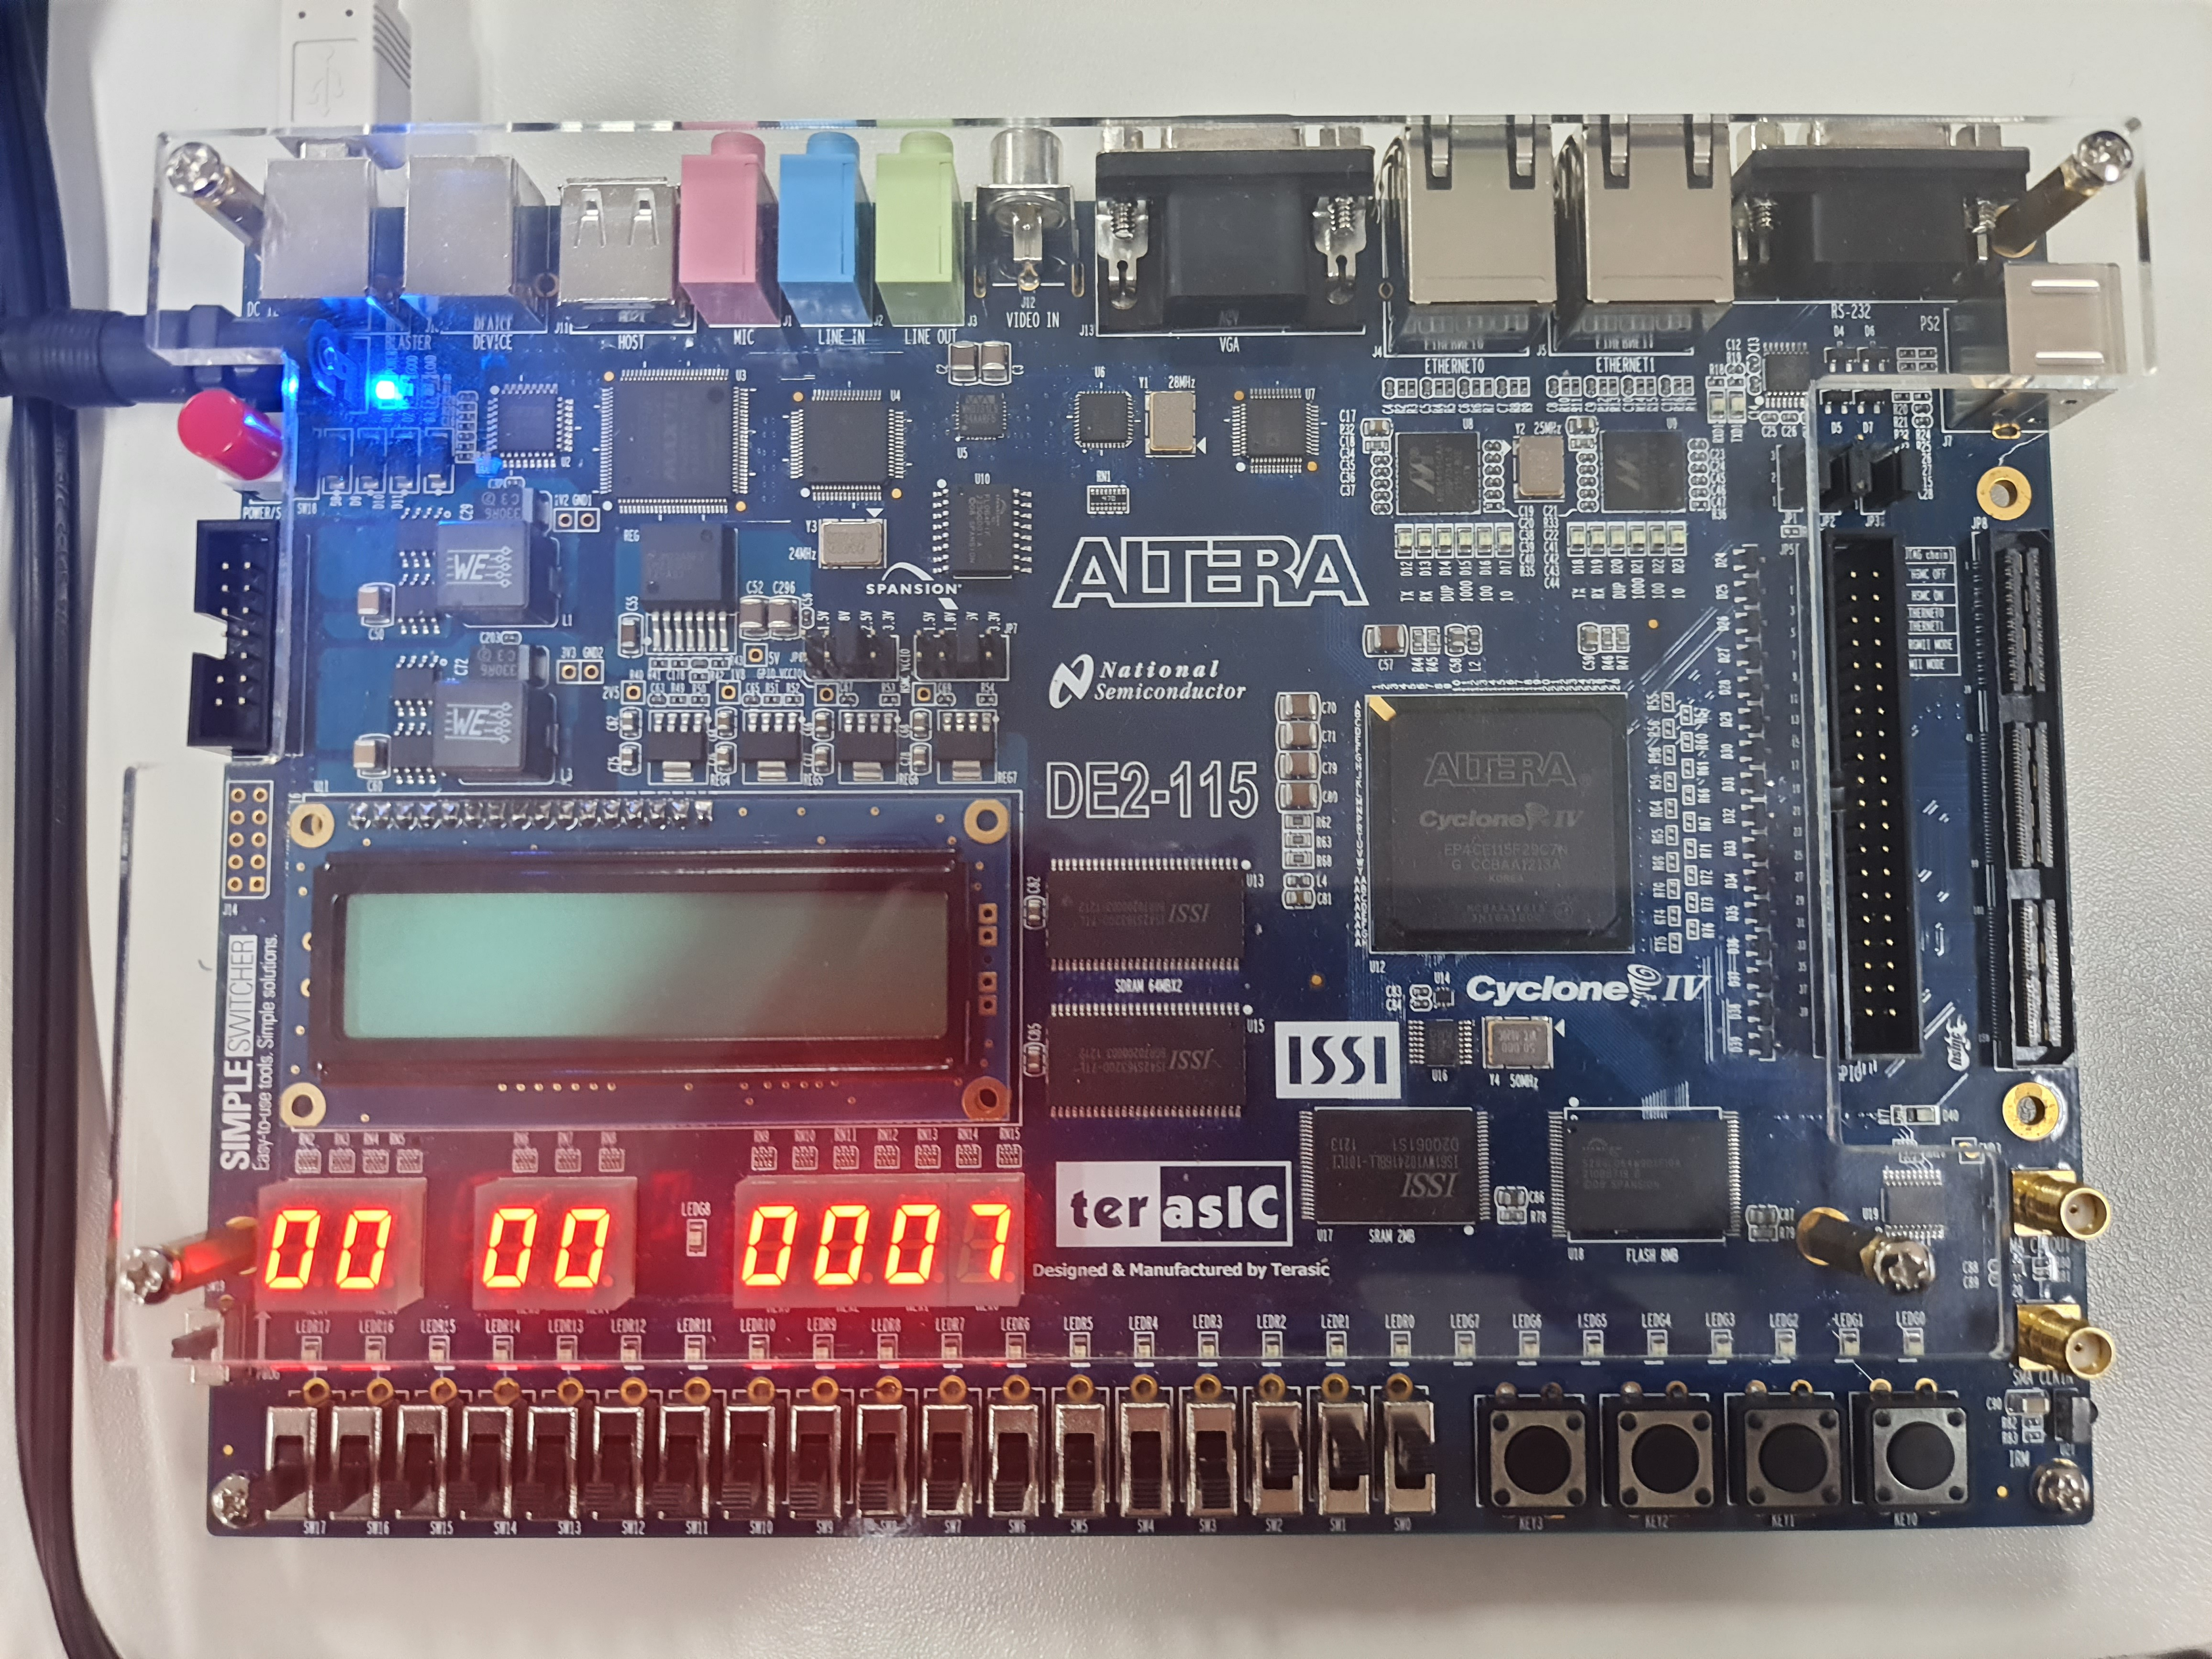
\includegraphics[width=0.7\textwidth]{Imagens/Processador_4.jpg} \\
  Fonte: o Autor.
  \label{fig:processador_4}
\end{figure}

\begin{figure}[H]
  \centering
  \caption{Número 4 e resultado - Código 2 - Calculo da média aritmética}
  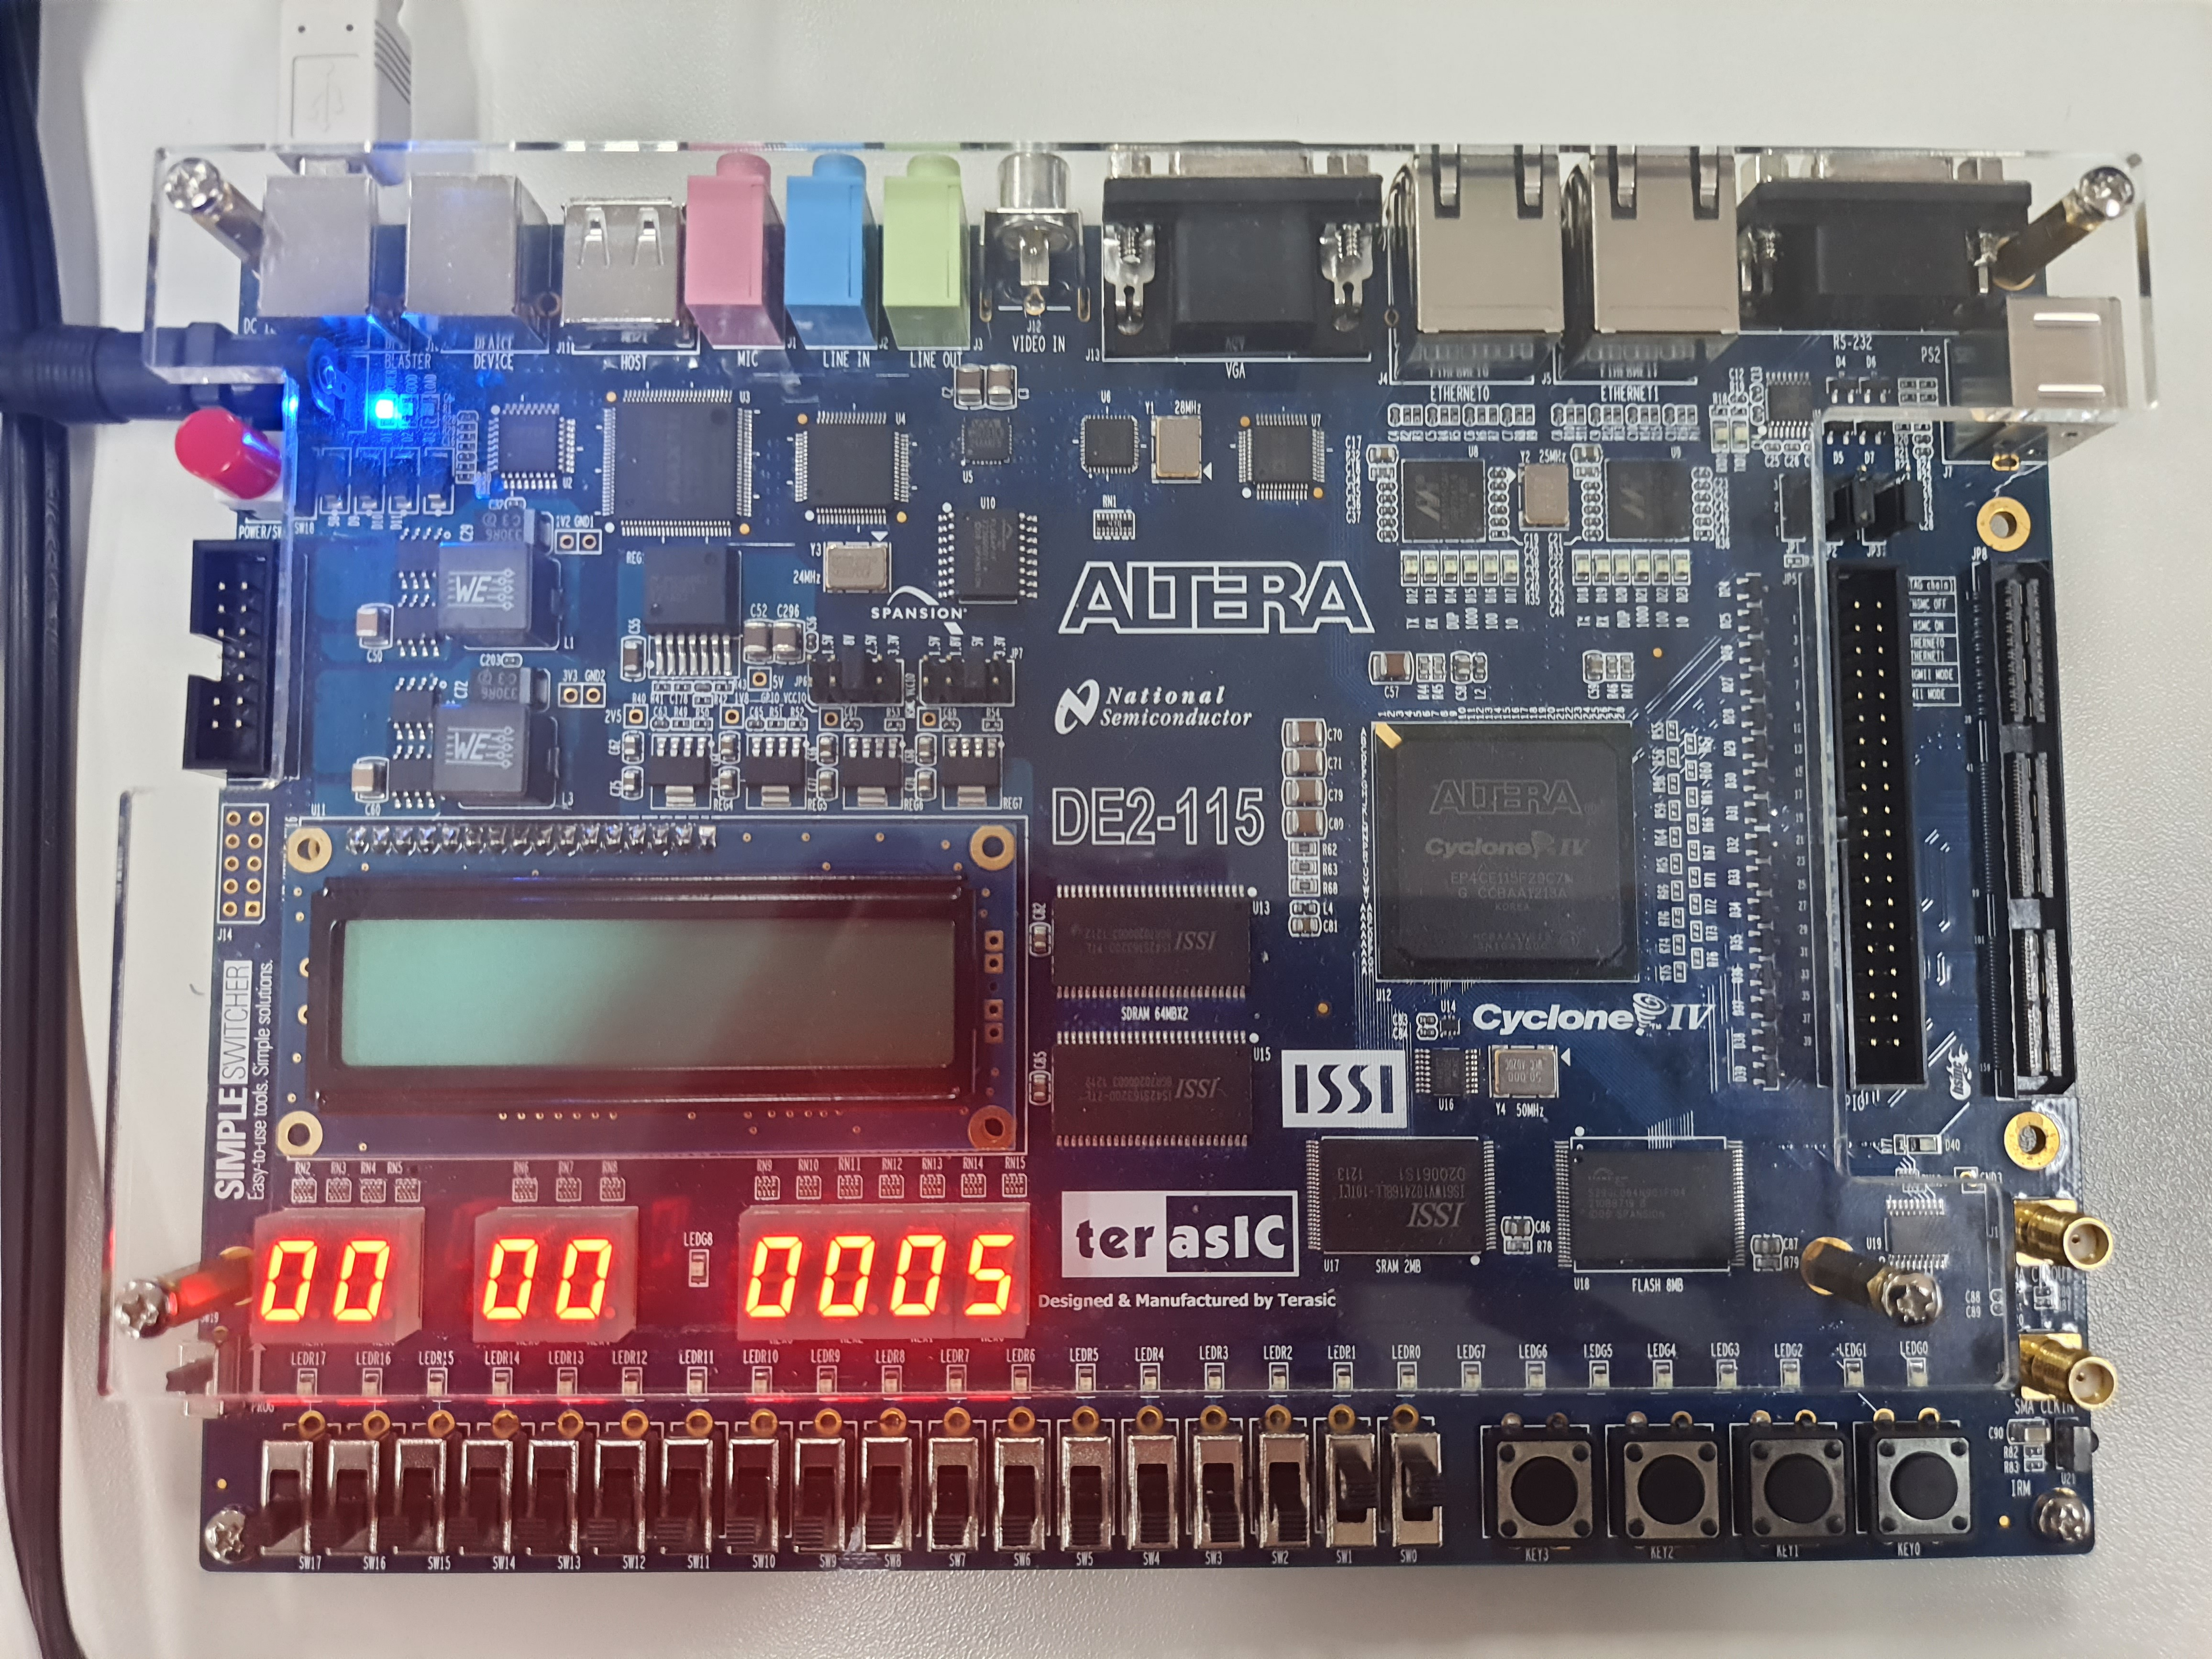
\includegraphics[width=0.7\textwidth]{Imagens/Processador_5.jpg} \\
  Fonte: o Autor.
  \label{fig:processador_5}
\end{figure}

% COMPILADOR: FASE DE ANÁLISE
\chapter{Compilador: Fase de Análise}
A fase de análise é o \textit{front-end} do compilador, ou seja, a parte responsável por ler o código-fonte em C-, entender a sua estrutura e verificar se ele está bem escrito. Ao final dessa fase, o programa deixa de ser um simples texto e passa a ser representado internamente por uma árvore sintática abstrata já validada, que serve de base para a fase de síntese. Essa fase é dividida em três etapas: a análise léxica, a análise sintática e a análise semântica \cite{louden2004}.

No projeto, a análise léxica foi construída com o auxílio da ferramenta Flex \cite{flex_manual}, que gera o analisador léxico a partir de um conjunto de expressões regulares, enquanto a análise sintática foi construída com o Bison \cite{bison_manual}, que gera um analisador sintático do tipo LALR a partir da gramática da linguagem. À medida que o analisador sintático reconhece a estrutura do programa, ele vai construindo a árvore sintática abstrata, que depois é percorrida pela análise semântica para montar a tabela de símbolos e verificar os tipos.

\section{Modelagem}
Antes da implementação, foi feita a modelagem da fase de análise utilizando a linguagem SysML, com o objetivo de organizar as ideias e representar tanto a estrutura quanto o comportamento dessa etapa do compilador.

\subsection{Diagrama de Blocos (SysML)}
\begin{quote}
\textit{Observação: o diagrama de blocos SysML referente à fase de análise não pôde ser incluído neste relatório. Devido a um problema pessoal com o meu computador, acabei perdendo os arquivos originais dos diagramas do compilador, não sendo possível recuperá-los a tempo da entrega. O conteúdo que esse diagrama representava está descrito ao longo das seções seguintes deste capítulo.}
\end{quote}

\subsection{Diagramas de Atividades (SysML)}
\begin{quote}
\textit{Observação: os diagramas de atividades SysML referentes à fase de análise também foram perdidos junto com os demais arquivos, pelo mesmo problema pessoal com o computador. O comportamento que esses diagramas descreviam, ou seja, o fluxo de reconhecimento dos tokens, a construção da árvore e as verificações semânticas, está explicado em texto nas seções a seguir.}
\end{quote}

\subsection{Outros: a Árvore Sintática Abstrata}
Além dos diagramas, uma estrutura central da fase de análise é a árvore sintática abstrata (AST). Ela representa o programa em forma de árvore, na qual cada nó corresponde a uma construção da linguagem, como uma declaração, uma expressão ou um comando. A definição do nó da árvore é apresentada no Código \ref{cod:ast}, onde é possível observar o tipo do nó, o tipo da expressão, os ponteiros para os filhos e para o próximo nó da lista, além dos campos usados para guardar números e identificadores.

\lstinputlisting[style=estiloC, caption={Definição do nó da árvore sintática abstrata (ast.h)}, label={cod:ast}]{codigos/ast_node.txt}

A escolha de usar um único tipo de nó com campos genéricos, ao invés de um tipo diferente para cada construção, deixa a árvore mais simples de percorrer, já que a fase de síntese pode tratar todos os nós de maneira uniforme, olhando apenas para o campo que indica o tipo do nó.

\section{Análise Léxica}
A análise léxica é a primeira etapa do compilador. Ela recebe o código-fonte como uma sequência de caracteres e agrupa esses caracteres em unidades com significado, chamadas de tokens, como palavras reservadas, identificadores, números e operadores. Ao mesmo tempo, ela descarta espaços em branco e comentários, e reporta os caracteres que não pertencem à linguagem.

O analisador léxico foi descrito no arquivo \texttt{scanner.l} utilizando o Flex. Cada regra associa uma expressão regular a uma ação, que normalmente devolve o token correspondente para o analisador sintático. O Código \ref{cod:scanner} mostra um trecho dessas regras, incluindo o tratamento das palavras reservadas, dos operadores, dos números, dos identificadores e dos comentários no formato \texttt{/* */}.

\lstinputlisting[style=estiloC, caption={Trecho das regras léxicas (scanner.l)}, label={cod:scanner}]{codigos/scanner_excerpt.txt}

Para os números, a ação converte o texto reconhecido em um valor inteiro com a função \texttt{atoi}, e para os identificadores é feita uma cópia do nome com \texttt{strdup}, de modo que esse nome possa ser usado depois na tabela de símbolos. Além disso, a cada token reconhecido, a linha atual é guardada por meio da macro \texttt{YY\_USER\_ACTION}, o que permite que os erros sejam reportados junto com o número da linha onde ocorreram. Quando o analisador encontra um caractere que não faz parte da linguagem, ele emite uma mensagem de erro léxico.

\section{Análise Sintática}
A análise sintática recebe a sequência de tokens produzida pela análise léxica e verifica se ela respeita a gramática da linguagem C-. Se a estrutura estiver correta, o analisador constrói a árvore sintática abstrata que representa o programa. Se não estiver, ele reporta um erro sintático.

Esse analisador foi descrito no arquivo \texttt{parser.y} com o Bison, que gera um analisador do tipo LALR. Um ponto importante na definição da gramática é a declaração de precedência e associatividade dos operadores, mostrada no Código \ref{cod:prec}. Nela, os operadores de soma e subtração recebem uma precedência menor do que os de multiplicação e divisão, o que garante que uma expressão como \texttt{a + b * c} seja interpretada da maneira esperada.

\lstinputlisting[style=estiloC, caption={Precedência e associatividade dos operadores (parser.y)}, label={cod:prec}]{codigos/parser_prec.txt}

Ainda sobre a precedência, foi utilizado o recurso de precedência para resolver a ambiguidade do \textit{dangling else}, ou seja, o problema de decidir a qual \texttt{if} um \texttt{else} pertence quando existem estruturas de decisão aninhadas. O Código \ref{cod:gram} apresenta um trecho das regras da gramática, onde é possível observar como as produções são associadas às ações que constroem a árvore. Cada vez que uma regra é reconhecida, um nó é criado e ligado aos seus filhos, montando a árvore de baixo para cima.

\lstinputlisting[style=estiloC, caption={Trecho da gramática e construção da árvore (parser.y)}, label={cod:gram}]{codigos/parser_grammar.txt}

Também foi adicionada uma forma simples de recuperação de erros, por meio de regras que usam o símbolo especial \texttt{error} seguido de \texttt{yyerrok}. Com isso, ao encontrar um erro em um comando, o analisador consegue descartar o trecho problemático e continuar a análise a partir do próximo ponto-e-vírgula, ao invés de parar na primeira falha.

\section{Análise Semântica}
A análise semântica é a etapa que verifica o significado do programa, indo além da sua estrutura. Nesse ponto, o compilador já sabe que o programa está bem formado do ponto de vista sintático, mas ainda precisa checar se ele faz sentido, como, por exemplo, se as variáveis foram declaradas antes de serem usadas, se as funções são chamadas com o número certo de argumentos e se os tipos são compatíveis.

Para isso, foi construída uma tabela de símbolos, responsável por guardar as informações de cada identificador do programa, como o seu tipo, a sua categoria, o escopo ao qual pertence e as linhas em que aparece. Essa tabela foi implementada como uma tabela \textit{hash}, cuja função de espalhamento é apresentada no Código \ref{cod:hash}.

\lstinputlisting[style=estiloC, caption={Função hash da tabela de símbolos (symtab.c)}, label={cod:hash}]{codigos/symtab_hash.txt}

A tabela de símbolos também trata os diferentes escopos do programa. Existe um escopo global, chamado de \texttt{Global}, e um escopo para cada função. A busca de um identificador é feita primeiro no escopo atual e, caso ele não seja encontrado, a busca continua no escopo global, o que permite que uma função enxergue tanto as suas próprias variáveis quanto as variáveis globais. O Código \ref{cod:insert} mostra a inserção de um símbolo na tabela, considerando o escopo atual.

\lstinputlisting[style=estiloC, caption={Inserção de um símbolo na tabela (symtab.c)}, label={cod:insert}]{codigos/symtab_insert.txt}

A verificação semântica é feita percorrendo a árvore sintática abstrata em duas etapas. Na primeira, a árvore é percorrida para preencher a tabela de símbolos, inserindo as declarações de variáveis e de funções, além das funções predefinidas \texttt{input} e \texttt{output}. Na segunda, a árvore é percorrida novamente para checar os tipos e reportar os erros semânticos. Entre as verificações feitas, estão a declaração de variáveis ou parâmetros do tipo \texttt{void}, a redeclaração de um mesmo identificador no mesmo escopo, o uso de identificadores não declarados, a chamada de funções com número ou tipo de argumentos incorretos, o uso indevido de vetores e a compatibilidade entre o tipo de retorno da função e o valor retornado. O Código \ref{cod:sem} mostra parte dessas verificações, incluindo a checagem dos tipos dos parâmetros em uma chamada de função e a checagem do tipo de retorno.

\lstinputlisting[style=estiloC, caption={Trecho da verificação de tipos (analyze.c)}, label={cod:sem}]{codigos/analyze_check.txt}

Por fim, ainda é verificado se a função \texttt{main} foi declarada, já que ela é o ponto de entrada do programa. Caso alguma dessas verificações falhe, o compilador reporta o erro correspondente junto com a linha em que ele ocorreu, e a compilação não avança para a fase de síntese.

% COMPILADOR: FASE DE SÍNTESE
\chapter{Compilador: Fase de Síntese}
A fase de síntese é o \textit{back-end} do compilador. Ela parte da árvore sintática abstrata já validada pela fase de análise e produz o código de saída, passando por três representações cada vez mais próximas do hardware: o código intermediário, o código assembly e o código binário. Além disso, essa fase também é responsável por decidir como as variáveis e os valores temporários serão guardados na memória e nos registradores do processador.

\section{Modelagem}
Assim como na fase de análise, a fase de síntese também foi modelada em SysML antes da implementação, buscando representar a estrutura das etapas de geração de código e o comportamento de cada uma delas.

\subsection{Diagrama de Blocos (SysML)}
\begin{quote}
\textit{Observação: o diagrama de blocos SysML referente à fase de síntese não pôde ser incluído neste relatório. Assim como os demais diagramas do compilador, ele foi perdido devido a um problema pessoal com o meu computador, não sendo possível recuperá-lo a tempo da entrega. A estrutura que esse diagrama representava está descrita ao longo deste capítulo.}
\end{quote}

\subsection{Diagramas de Atividades (SysML)}
\begin{quote}
\textit{Observação: os diagramas de atividades SysML referentes à fase de síntese também foram perdidos pelo mesmo motivo. O fluxo de geração do código intermediário, do assembly e do binário que esses diagramas descreviam está explicado em texto nas seções seguintes.}
\end{quote}

\section{Geração de Código Intermediário}
O código intermediário é uma representação que fica entre a linguagem de alto nível e o código de máquina \cite{aho2008}. Ele é independente dos detalhes do processador, o que facilita tanto a geração do código quanto a sua leitura durante os testes. No projeto, essa representação foi feita por meio de quádruplas, que são instruções compostas por uma operação e três endereços.

O Código \ref{cod:quad} apresenta os tipos usados na representação intermediária. A estrutura \texttt{Quad} guarda a operação e os três endereços, além de um ponteiro para a próxima quádrupla, formando uma lista encadeada. Cada endereço, representado pela estrutura \texttt{Address}, possui um campo que indica o seu tipo, que pode ser uma constante inteira, uma variável, um temporário, um rótulo ou um registrador, além do seu valor e do seu nome.

\lstinputlisting[style=estiloC, caption={Tipos da representação intermediária (cintgen.h)}, label={cod:quad}]{codigos/cintgen_types.txt}

As operações possíveis nas quádruplas cobrem as principais construções da linguagem. A Tabela \ref{tab:quad} organiza esses tipos de quádrupla em categorias, mostrando o papel de cada grupo na representação intermediária.

\begin{table}[H]
\centering
\caption{Tipos de quádrupla gerados pelo compilador}
\label{tab:quad}
\begin{tabular}{|l|l|}
\hline
\textbf{Categoria} & \textbf{Operações} \\
\hline
Aritméticas & \texttt{add}, \texttt{sub}, \texttt{mul}, \texttt{div} (e suas variantes com imediato e registrador) \\
\hline
Desvios condicionais & \texttt{blt}, \texttt{ble}, \texttt{bgt}, \texttt{bge}, \texttt{beq}, \texttt{bne} \\
\hline
Controle de fluxo & \texttt{iff}, \texttt{jmp}, \texttt{jr}, \texttt{lab} \\
\hline
Funções & \texttt{fun}, \texttt{end}, \texttt{arg}, \texttt{param}, \texttt{call}, \texttt{ret} \\
\hline
Memória e cópia & \texttt{alloc}, \texttt{free}, \texttt{load}, \texttt{loaddi}, \texttt{store}, \texttt{storedi}, \texttt{mov}, \texttt{movi}, \texttt{movr} \\
\hline
Entrada e saída & \texttt{in}, \texttt{out} \\
\hline
Encerramento & \texttt{halt} \\
\hline
\end{tabular}
\end{table}

As quádruplas são criadas por meio da função \texttt{makeNewQuad}, mostrada no Código \ref{cod:makequad}. Essa função aloca uma nova quádrupla, preenche a operação e os endereços e a adiciona ao final da lista encadeada. Além disso, sempre que um dos endereços é um temporário, ela atualiza uma lista de controle que acompanha o uso dos temporários, informação que é importante depois, na alocação de registradores.

\lstinputlisting[style=estiloC, caption={Criação de uma quádrupla (cintgen.c)}, label={cod:makequad}]{codigos/cintgen_makequad.txt}

A geração do código intermediário é feita percorrendo a árvore sintática abstrata por meio de uma grande estrutura de decisão, na qual cada tipo de nó gera as quádruplas correspondentes. O Código \ref{cod:if} mostra o tratamento de uma estrutura de decisão \texttt{if/else}, no qual são criados os rótulos para o desvio e para o fim da estrutura, e são gerados os saltos que ligam o teste da condição, o bloco do \texttt{if} e o bloco do \texttt{else}.

\lstinputlisting[style=estiloC, caption={Geração de código para o if/else (cintgen.c)}, label={cod:if}]{codigos/cintgen_if.txt}

\section{Geração de Código Assembly}
A geração de código assembly transforma as quádruplas em instruções da linguagem de montagem do processador. Nessa etapa, dois problemas principais precisam ser resolvidos: decidir em quais registradores os valores serão guardados e traduzir cada quádrupla para a instrução correta.

O processador possui um número limitado de registradores de uso geral, então a alocação de registradores precisa reaproveitá-los ao longo do programa. O Código \ref{cod:alloc} mostra a função responsável por essa alocação. Ela primeiro verifica se o temporário já está em algum registrador e, caso esteja, apenas o reutiliza. Caso contrário, ela procura um registrador livre, identificado por uma soma de usos igual a zero, e o associa ao novo temporário.

\lstinputlisting[style=estiloC, caption={Alocação de registradores (casm.c)}, label={cod:alloc}]{codigos/casm_alloc.txt}

Outro ponto importante dessa etapa é que algumas operações da representação intermediária são genéricas e precisam ser especializadas de acordo com o tipo dos seus operandos. O Código \ref{cod:conv} mostra essa conversão para as operações aritméticas. Uma operação de soma, por exemplo, é transformada em uma instrução com imediato quando o terceiro operando é uma constante, ou em uma instrução entre registradores quando o operando é um temporário ou um registrador.

\lstinputlisting[style=estiloC, caption={Especialização das operações aritméticas (casm.c)}, label={cod:conv}]{codigos/casm_conv.txt}

\section{Geração de Código Executável}
A última etapa da fase de síntese é a geração do código executável, ou seja, o código binário que o processador consegue interpretar diretamente. Cada instrução assembly é convertida em uma palavra de 32 bits, na qual os primeiros 6 bits representam o \textit{opcode}, que identifica a operação, e os bits restantes representam os operandos, de acordo com o formato da instrução.

O Código \ref{cod:opcode} mostra a função que associa cada operação ao seu \textit{opcode} de 6 bits. Esses valores seguem exatamente os códigos definidos no processador desenvolvido anteriormente, garantindo que o binário gerado pelo compilador seja compatível com o hardware.

\lstinputlisting[style=estiloC, caption={Opcodes das instruções (binary.c)}, label={cod:opcode}]{codigos/binary_opcode.txt}

A montagem final da palavra de 32 bits leva em conta o formato de cada instrução, distribuindo os bits entre os registradores e os valores imediatos. Um cuidado especial é necessário nos desvios, cujo destino é calculado como um deslocamento relativo em relação à próxima instrução, ou seja, o rótulo de destino menos a posição do \texttt{PC} somada de um. O Código \ref{cod:bingen} mostra parte dessa montagem.

\lstinputlisting[style=estiloC, caption={Montagem das instruções binárias (binary.c)}, label={cod:bingen}]{codigos/binary_gen.txt}

\section{Gerenciamento de Memória}
Como o processador tem uma quantidade pequena de registradores, boa parte das variáveis e dos parâmetros das funções precisa ser guardada na memória. Para organizar esse uso, o gerenciamento de memória foi feito com base em duas pilhas, que crescem em sentido decrescente a partir do topo da memória.

A memória disponível é definida por uma constante de tamanho igual a 127. A partir desse valor, o registrador \texttt{R13} funciona como ponteiro da pilha global, onde ficam as variáveis globais, e o registrador \texttt{R12} funciona como ponteiro da pilha geral, usada durante a execução das funções para guardar variáveis locais, parâmetros e valores temporários. No início do programa, o ponteiro global é inicializado com o topo da memória, por meio da instrução \texttt{movi R13, 127}, e o ponteiro geral é inicializado com o mesmo valor, por meio da instrução \texttt{movr R12, R13}.

Para alocar espaço em uma pilha, o ponteiro correspondente é decrementado com a instrução \texttt{subi}, e para liberar esse espaço, o ponteiro é incrementado de volta com a instrução \texttt{addi}. Dessa forma, cada função aloca o espaço de que precisa ao ser chamada e libera esse espaço ao retornar, o que permite inclusive o funcionamento correto da recursão, já que cada chamada trabalha com a sua própria região da pilha.

% EXEMPLOS
\chapter{Exemplos}
Para demonstrar o funcionamento completo do compilador, esta seção apresenta três exemplos de programas escritos em C-, com complexidade crescente. Para cada exemplo, são mostrados o código-fonte, o código intermediário, o código assembly e o código binário gerados pelo compilador. No final do capítulo, são apresentadas as correspondências entre essas representações, usando o exemplo mais simples para facilitar o acompanhamento.

\section{Exemplo 1: Programa Simples}
O primeiro exemplo é um programa curto, que declara um vetor e uma variável, chama uma função que apenas devolve o seu parâmetro e usa o resultado em uma soma. Apesar de simples, ele já exercita a declaração de vetores, a chamada de função com parâmetro e o uso de variáveis locais.

\lstinputlisting[style=estiloC, caption={Exemplo 1: código-fonte (simples.txt)}]{codigos/simples_src.txt}

O código intermediário correspondente é mostrado a seguir. Nele, é possível observar as quádruplas de declaração das funções, de alocação das variáveis, de carga dos valores, de passagem de parâmetro, de chamada e de soma.

\lstinputlisting[style=estiloTexto, caption={Exemplo 1: código intermediário}]{codigos/simples_int.txt}

O código assembly gerado, já com os registradores alocados e as instruções especializadas, é apresentado a seguir.

\lstinputlisting[style=estiloTexto, caption={Exemplo 1: código assembly}]{codigos/simples_asm.txt}

Por fim, o código binário, com cada instrução representada por uma palavra de 32 bits, é mostrado a seguir.

\lstinputlisting[style=estiloTexto, caption={Exemplo 1: código binário}]{codigos/simples_bin.txt}

\section{Exemplo 2: Fatorial com Recursão}
O segundo exemplo calcula o fatorial de um número utilizando recursão. Ele exercita a estrutura de decisão \texttt{if/else}, a chamada recursiva de uma função e o uso da entrada e da saída por meio das funções \texttt{input} e \texttt{output}.

\lstinputlisting[style=estiloC, caption={Exemplo 2: código-fonte (fatorial.txt)}]{codigos/fatorial_src.txt}

\lstinputlisting[style=estiloTexto, caption={Exemplo 2: código intermediário}]{codigos/fatorial_int.txt}

\lstinputlisting[style=estiloTexto, caption={Exemplo 2: código assembly}]{codigos/fatorial_asm.txt}

\lstinputlisting[style=estiloTexto, caption={Exemplo 2: código binário}]{codigos/fatorial_bin.txt}

\section{Exemplo 3: Máximo Divisor Comum}
O terceiro exemplo calcula o máximo divisor comum de dois números pelo algoritmo de Euclides. Ele combina recursão, estrutura de decisão e várias operações aritméticas em uma mesma expressão, sendo o exemplo mais completo dos três.

\lstinputlisting[style=estiloC, caption={Exemplo 3: código-fonte (gcd.txt)}]{codigos/gcd_src.txt}

\lstinputlisting[style=estiloTexto, caption={Exemplo 3: código intermediário}]{codigos/gcd_int.txt}

\lstinputlisting[style=estiloTexto, caption={Exemplo 3: código assembly}]{codigos/gcd_asm.txt}

\lstinputlisting[style=estiloTexto, caption={Exemplo 3: código binário}]{codigos/gcd_bin.txt}

\section{Correspondência entre as Representações}
Para tornar mais clara a relação entre as diferentes saídas do compilador, esta seção usa o primeiro exemplo para mostrar como cada trecho do programa é traduzido de uma representação para a outra.

\subsection{Correspondência entre o Código-Fonte e o Código Intermediário}
A Tabela \ref{tab:corr1} relaciona cada trecho do código-fonte do primeiro exemplo com as quádruplas geradas para ele. É possível observar como uma única linha de código de alto nível pode dar origem a várias quádruplas, especialmente quando envolve chamadas de função e operações aritméticas.

\begin{table}[H]
\centering
\caption{Correspondência entre o código-fonte e o código intermediário (Exemplo 1)}
\label{tab:corr1}
\begin{tabular}{|l|l|}
\hline
\textbf{Código-fonte} & \textbf{Código intermediário} \\
\hline
\texttt{int bla(int b)} & \texttt{(fun, int, bla, -)} e \texttt{(arg, b, 1, bla)} \\
\hline
\texttt{return b;} & \texttt{(load, t0, b, 0)} e \texttt{(ret, t0, -, -)} \\
\hline
\texttt{int vet[10];} & \texttt{(alloc, vet, 10, main)} \\
\hline
\texttt{int y;} & \texttt{(alloc, y, 1, main)} \\
\hline
\texttt{y = y + bla(y);} & \texttt{(load, t1, y, 0)}, \texttt{(load, t2, y, 0)}, \texttt{(param, t2, -, -)}, \\
 & \texttt{(call, t3, bla, 1)}, \texttt{(add, t4, t1, t3)}, \texttt{(store, y, t4, 0)} \\
\hline
\texttt{return;} & \texttt{(ret, -, -, -)} \\
\hline
\end{tabular}
\end{table}

\subsection{Correspondência entre o Código Intermediário e o Código Assembly}
A Tabela \ref{tab:corr2} relaciona algumas quádruplas do primeiro exemplo com as instruções assembly geradas para elas. Nessa tradução, é possível notar a alocação dos registradores e a especialização das operações, como a soma que se torna uma instrução entre registradores.

\begin{table}[H]
\centering
\caption{Correspondência entre o código intermediário e o código assembly (Exemplo 1)}
\label{tab:corr2}
\begin{tabular}{|l|l|}
\hline
\textbf{Código intermediário} & \textbf{Código assembly} \\
\hline
\texttt{(alloc, y, 1, main)} & \texttt{subi R12, R12, 1} \\
\hline
\texttt{(load, t1, y, 0)} & \texttt{loaddi R1, R12, 1} \\
\hline
\texttt{(param, t2, -, -)} & \texttt{subi R12, R12, 1} e \texttt{storedi R12, R2, 1} \\
\hline
\texttt{(call, t3, bla, 1)} & \texttt{movi R3, L2}, \texttt{subi R12, R12, 1}, \texttt{storedi R12, R3, 1}, \texttt{jmp L0} \\
\hline
\texttt{(add, t4, t1, t3)} & \texttt{addr R3, R1, R2} \\
\hline
\end{tabular}
\end{table}

Com esses exemplos, é possível acompanhar o caminho completo percorrido por um programa, desde o código escrito em C- até as instruções em binário que serão executadas pelo processador, passando por cada uma das representações intermediárias geradas pelo compilador.

% CONSIDERAÇÕES FINAIS
\chapter{Conclusão}
Ao longo deste relatório, foi apresentado o desenvolvimento de um compilador para a linguagem C-, capaz de traduzir um programa de alto nível até o código binário, além do processador MIPS monociclo que serve de alvo para esse código e que foi desenvolvido anteriormente. Com isso, tornou-se possível acompanhar todo o caminho de um programa, desde a sua escrita em C- até a execução das instruções em binário no hardware, passando pela análise léxica, sintática e semântica e, em seguida, pela geração do código intermediário, do assembly e do executável.

\section{Dificuldades Encontradas}
Durante o desenvolvimento do compilador, uma das maiores dificuldades foi a alocação de registradores, já que o processador possui uma quantidade pequena de registradores de uso geral. Foi preciso criar uma forma de reaproveitá-los ao longo do programa e de decidir quando um valor deveria ser guardado na memória para liberar espaço, o que exigiu bastante atenção para não sobrescrever um valor que ainda seria utilizado.

Ligada a essa questão, também foi trabalhosa a situação dos valores temporários que precisam sobreviver a uma chamada de função, pois eles não podem simplesmente ficar em um registrador que a função chamada pode alterar. Para tratar esse caso, foi necessário acompanhar o uso de cada temporário e proteger aqueles que atravessam uma chamada.

Outro ponto que gerou dificuldade foi o gerenciamento de memória com as duas pilhas, principalmente para garantir o funcionamento correto da recursão, na qual cada chamada precisa da sua própria região de memória. Além disso, na geração do código binário, foi preciso ter cuidado no cálculo do destino dos desvios, que é feito de forma relativa em relação à próxima instrução, e na conversão das quádruplas genéricas para o formato de instrução correto de acordo com o tipo dos operandos.

Em relação ao processador, durante o seu desenvolvimento, foram encontradas algumas contradições entre a operação realizada pelas instruções storer e storei e o caminho de dados. Além disso, o salto condicional a princípio não estava considerando a posição atual do PC. Ambos os erros já foram corrigidos.

Ainda sobre o processador, inicialmente estava planejado executar as operações de multiplicação e divisão utilizando dois registradores especiais para armazenar o resultado, RH, para a parte alta da multiplicação e RL, para a parte baixa da multiplicação. Porém, constatou-se que isso iria fazer a utilização do processador ser consideravelmente mais complicada. Isso levou a uma mudança para permitir que a parte baixa do resultado pudesse ser escrita em qualquer registrador. Foi também abandonada a ideia de utilizar o registrador específico RH, pois, durante o desenvolvimento da integração entre a ULA e o banco de registradores, foi observado que o tempo de compilação aumentava de cerca de 11 minutos para meia hora ao utilizar duas conexões entre a ULA e o banco de registradores. Sendo assim, o projeto passou a utilizar somente a saída padrão, SL, para essas instruções.

Além disso, para receber e enviar dados para o módulo de entrada e saída, a princípio, seriam utilizados exclusivamente dois registradores especiais, RIN, para receber os dados, e ROUT para enviar. Todavia, isso também poderia dificultar a utilização do processador futuramente, então passou a ser permitido que qualquer registrador desempenhe essas funções. Um outro desafio encontrado foi o caminho de dados, que originalmente havia sido desenvolvido de um modo muito ineficiente. Desse modo, foi preciso corrigi-lo, tanto para ser mais fácil de compreendê-lo quanto para ser mais simples de implementá-lo. Por fim, na etapa de testes no kit FPGA, foram encontradas grandes dificuldades para escrever corretamente os valores no display, já que o valor era escrito em um ciclo de clock e perdido no ciclo seguinte. Após muitos testes, a solução encontrada foi escrever no display somente durante a borda de descida do clock.

\section{Destaques}
Um dos principais destaques do projeto é o fato de o compilador funcionar de ponta a ponta, ou seja, ele recebe um programa em C- e produz, de forma automática, o código intermediário, o código assembly e o código binário correspondente. Além disso, o binário gerado utiliza exatamente os mesmos opcodes e formatos do processador desenvolvido anteriormente, o que permite que o código produzido pelo compilador seja de fato executado no hardware implementado no kit FPGA.

Outro ponto de destaque é o suporte à recursão, que pôde ser demonstrado nos exemplos do fatorial e do máximo divisor comum. Poder acompanhar um mesmo programa em todas as suas representações, desde o código-fonte até o binário, ajuda bastante a entender de maneira concreta como um compilador transforma um programa de alto nível em algo que a máquina consegue executar. Em relação ao processador, vale destacar que todos os módulos desenvolvidos foram testados e apresentaram o funcionamento de acordo com o planejado, e a integração entre eles foi feita aos poucos, sem grandes problemas.

\section{Trabalhos Futuros}
No compilador, muitas melhorias ainda poderiam ser feitas. Seria interessante aplicar otimizações ao código gerado, de modo a reduzir a quantidade de instruções produzidas, além de aprimorar a alocação de registradores e o controle dos valores temporários. Também seria possível ampliar o conjunto de construções da linguagem tratadas pelo compilador e melhorar as mensagens de erro apresentadas ao usuário.

Já no processador, muitas melhorias poderiam ser feitas, incluindo: uma melhor organização do caminho de dados, que poderia ser mais simples e direto; ao invés de escrever em dois registradores ao mesmo tempo no banco, transformar os registradores especiais em buffers que ficariam dentro do módulo onde são usados; teste de mais instruções para garantir ainda mais solidamente o correto funcionamento.

% ---
% Finaliza a parte no bookmark do PDF
% para que se inicie o bookmark na raiz
% e adiciona espaço de parte no Sumário
% ---
\phantompart


% --------------------------ELEMENTOS PÓS-TEXTUAIS----------------------
\postextual

% ------------------------Referências bibliográficas--------------------
\bibliography{referencias}



\end{document}